\chapter{Computational experiments and discussion}\label{results}

This chapter is divided into two parts. The first part deals with the evaluation of the computational performance of the high level programming language Python. Here, we discuss the task of evaluating the ground state energy of a quantum mechanical system by the Quantum Variational Monte Carlo (QVMC) method. In the second part, we use an optimized version of the QVMC simulator to evaluate the ground state energies of He, Be and two dimensional quantum dots with two and six electrons.

\section{Comparing high to low level programming languages in a QVMC application}

A prototype in Python capable of computing the ground state energy of the helium (He) atom 
by the QVMC method with importance sampling was developed and discussed in section \ref{PythonPrototype}. Results of simulations for a similar implementation in C++ are shown figure \ref{energyHePlainCpp}. The experiment was carried out with 10 millions Monte Carlo cycles using importance sampling. \\
\\
To determine the ground state energy of the system, the variational parameter $\alpha$ was set equal to the effective nuclear charge\footnote{The effective charge is the net positive charge experienced by an electron in a multi-electron atom. Because of the presence of other electrons, the ones in higher orbitals do not experience the full nuclear charge due to the shielding effect. The value $Z_{eff} = 1.6785$ is taken from Clementi(1963)\cite{Clementi1963}}. Then, 40 variations of $\beta$ in the range $0.1-1.2$ were carried out. The ground state energy was estimated to be $E_0 = -2.8731096 \pm 1.9705\times10^{-4} \, au$ with $\beta_{optimum} \approx 0.45$ by selecting the point with the lowest variance. The given value should be compared with table \ref{energiesHePythonVsRef}. We should pay attention to the fact that the lowest energy does not necessarily means that we obtain lowest variance as well, as indicated by the error bars appearing in the box inside figure \ref{energyHePlainCpp}.\\


\begin{figure}
\centering
\scalebox{0.75}{\begin{tikzpicture}[gnuplot]
%% generated with GNUPLOT 4.2p5  (Lua 5.1.4; terminal rev. 81, script rev. 88)
%% Mon Sep  7 13:53:42 2009
\color{gp_lt_color_b}
\gpsetlinetype{gp_lt_border}
\gpsetlinewidth{1.00}
\draw[gp path] (2.056,0.985)--(2.236,0.985);
\draw[gp path] (12.040,0.985)--(11.860,0.985);
\node[gp node right] at (1.872,0.985) {-2.88};
\draw[gp path] (2.056,1.108)--(2.146,1.108);
\draw[gp path] (12.040,1.108)--(11.950,1.108);
\draw[gp path] (2.056,1.232)--(2.146,1.232);
\draw[gp path] (12.040,1.232)--(11.950,1.232);
\draw[gp path] (2.056,1.355)--(2.146,1.355);
\draw[gp path] (12.040,1.355)--(11.950,1.355);
\draw[gp path] (2.056,1.478)--(2.146,1.478);
\draw[gp path] (12.040,1.478)--(11.950,1.478);
\draw[gp path] (2.056,1.601)--(2.146,1.601);
\draw[gp path] (12.040,1.601)--(11.950,1.601);
\draw[gp path] (2.056,1.725)--(2.146,1.725);
\draw[gp path] (12.040,1.725)--(11.950,1.725);
\draw[gp path] (2.056,1.848)--(2.146,1.848);
\draw[gp path] (12.040,1.848)--(11.950,1.848);
\draw[gp path] (2.056,1.971)--(2.146,1.971);
\draw[gp path] (12.040,1.971)--(11.950,1.971);
\draw[gp path] (2.056,2.095)--(2.146,2.095);
\draw[gp path] (12.040,2.095)--(11.950,2.095);
\draw[gp path] (2.056,2.218)--(2.236,2.218);
\draw[gp path] (12.040,2.218)--(11.860,2.218);
\node[gp node right] at (1.872,2.218) {-2.87};
\draw[gp path] (2.056,2.341)--(2.146,2.341);
\draw[gp path] (12.040,2.341)--(11.950,2.341);
\draw[gp path] (2.056,2.464)--(2.146,2.464);
\draw[gp path] (12.040,2.464)--(11.950,2.464);
\draw[gp path] (2.056,2.588)--(2.146,2.588);
\draw[gp path] (12.040,2.588)--(11.950,2.588);
\draw[gp path] (2.056,2.711)--(2.146,2.711);
\draw[gp path] (12.040,2.711)--(11.950,2.711);
\draw[gp path] (2.056,2.834)--(2.146,2.834);
\draw[gp path] (12.040,2.834)--(11.950,2.834);
\draw[gp path] (2.056,2.958)--(2.146,2.958);
\draw[gp path] (12.040,2.958)--(11.950,2.958);
\draw[gp path] (2.056,3.081)--(2.146,3.081);
\draw[gp path] (12.040,3.081)--(11.950,3.081);
\draw[gp path] (2.056,3.204)--(2.146,3.204);
\draw[gp path] (12.040,3.204)--(11.950,3.204);
\draw[gp path] (2.056,3.327)--(2.146,3.327);
\draw[gp path] (12.040,3.327)--(11.950,3.327);
\draw[gp path] (2.056,3.451)--(2.236,3.451);
\draw[gp path] (12.040,3.451)--(11.860,3.451);
\node[gp node right] at (1.872,3.451) {-2.86};
\draw[gp path] (2.056,3.574)--(2.146,3.574);
\draw[gp path] (12.040,3.574)--(11.950,3.574);
\draw[gp path] (2.056,3.697)--(2.146,3.697);
\draw[gp path] (12.040,3.697)--(11.950,3.697);
\draw[gp path] (2.056,3.821)--(2.146,3.821);
\draw[gp path] (12.040,3.821)--(11.950,3.821);
\draw[gp path] (2.056,3.944)--(2.146,3.944);
\draw[gp path] (12.040,3.944)--(11.950,3.944);
\draw[gp path] (2.056,4.067)--(2.146,4.067);
\draw[gp path] (12.040,4.067)--(11.950,4.067);
\draw[gp path] (2.056,4.190)--(2.146,4.190);
\draw[gp path] (12.040,4.190)--(11.950,4.190);
\draw[gp path] (2.056,4.314)--(2.146,4.314);
\draw[gp path] (12.040,4.314)--(11.950,4.314);
\draw[gp path] (2.056,4.437)--(2.146,4.437);
\draw[gp path] (12.040,4.437)--(11.950,4.437);
\draw[gp path] (2.056,4.560)--(2.146,4.560);
\draw[gp path] (12.040,4.560)--(11.950,4.560);
\draw[gp path] (2.056,4.683)--(2.236,4.683);
\draw[gp path] (12.040,4.683)--(11.860,4.683);
\node[gp node right] at (1.872,4.683) {-2.85};
\draw[gp path] (2.056,4.807)--(2.146,4.807);
\draw[gp path] (12.040,4.807)--(11.950,4.807);
\draw[gp path] (2.056,4.930)--(2.146,4.930);
\draw[gp path] (12.040,4.930)--(11.950,4.930);
\draw[gp path] (2.056,5.053)--(2.146,5.053);
\draw[gp path] (12.040,5.053)--(11.950,5.053);
\draw[gp path] (2.056,5.177)--(2.146,5.177);
\draw[gp path] (12.040,5.177)--(11.950,5.177);
\draw[gp path] (2.056,5.300)--(2.146,5.300);
\draw[gp path] (12.040,5.300)--(11.950,5.300);
\draw[gp path] (2.056,5.423)--(2.146,5.423);
\draw[gp path] (12.040,5.423)--(11.950,5.423);
\draw[gp path] (2.056,5.546)--(2.146,5.546);
\draw[gp path] (12.040,5.546)--(11.950,5.546);
\draw[gp path] (2.056,5.670)--(2.146,5.670);
\draw[gp path] (12.040,5.670)--(11.950,5.670);
\draw[gp path] (2.056,5.793)--(2.146,5.793);
\draw[gp path] (12.040,5.793)--(11.950,5.793);
\draw[gp path] (2.056,5.916)--(2.236,5.916);
\draw[gp path] (12.040,5.916)--(11.860,5.916);
\node[gp node right] at (1.872,5.916) {-2.84};
\draw[gp path] (2.056,6.040)--(2.146,6.040);
\draw[gp path] (12.040,6.040)--(11.950,6.040);
\draw[gp path] (2.056,6.163)--(2.146,6.163);
\draw[gp path] (12.040,6.163)--(11.950,6.163);
\draw[gp path] (2.056,6.286)--(2.146,6.286);
\draw[gp path] (12.040,6.286)--(11.950,6.286);
\draw[gp path] (2.056,6.409)--(2.146,6.409);
\draw[gp path] (12.040,6.409)--(11.950,6.409);
\draw[gp path] (2.056,6.533)--(2.146,6.533);
\draw[gp path] (12.040,6.533)--(11.950,6.533);
\draw[gp path] (2.056,6.656)--(2.146,6.656);
\draw[gp path] (12.040,6.656)--(11.950,6.656);
\draw[gp path] (2.056,6.779)--(2.146,6.779);
\draw[gp path] (12.040,6.779)--(11.950,6.779);
\draw[gp path] (2.056,6.903)--(2.146,6.903);
\draw[gp path] (12.040,6.903)--(11.950,6.903);
\draw[gp path] (2.056,7.026)--(2.146,7.026);
\draw[gp path] (12.040,7.026)--(11.950,7.026);
\draw[gp path] (2.056,7.149)--(2.236,7.149);
\draw[gp path] (12.040,7.149)--(11.860,7.149);
\node[gp node right] at (1.872,7.149) {-2.83};
\draw[gp path] (2.056,7.272)--(2.146,7.272);
\draw[gp path] (12.040,7.272)--(11.950,7.272);
\draw[gp path] (2.056,7.396)--(2.146,7.396);
\draw[gp path] (12.040,7.396)--(11.950,7.396);
\draw[gp path] (2.056,7.519)--(2.146,7.519);
\draw[gp path] (12.040,7.519)--(11.950,7.519);
\draw[gp path] (2.056,7.642)--(2.146,7.642);
\draw[gp path] (12.040,7.642)--(11.950,7.642);
\draw[gp path] (2.056,7.766)--(2.146,7.766);
\draw[gp path] (12.040,7.766)--(11.950,7.766);
\draw[gp path] (2.056,7.889)--(2.146,7.889);
\draw[gp path] (12.040,7.889)--(11.950,7.889);
\draw[gp path] (2.056,8.012)--(2.146,8.012);
\draw[gp path] (12.040,8.012)--(11.950,8.012);
\draw[gp path] (2.056,8.135)--(2.146,8.135);
\draw[gp path] (12.040,8.135)--(11.950,8.135);
\draw[gp path] (2.056,8.259)--(2.146,8.259);
\draw[gp path] (12.040,8.259)--(11.950,8.259);
\draw[gp path] (2.056,8.382)--(2.236,8.382);
\draw[gp path] (12.040,8.382)--(11.860,8.382);
\node[gp node right] at (1.872,8.382) {-2.82};
\draw[gp path] (2.056,0.985)--(2.056,1.165);
\draw[gp path] (2.056,8.382)--(2.056,8.202);
\node[gp node center] at (2.056,0.677) {0};
\draw[gp path] (2.222,0.985)--(2.222,1.075);
\draw[gp path] (2.222,8.382)--(2.222,8.292);
\draw[gp path] (2.389,0.985)--(2.389,1.075);
\draw[gp path] (2.389,8.382)--(2.389,8.292);
\draw[gp path] (2.555,0.985)--(2.555,1.075);
\draw[gp path] (2.555,8.382)--(2.555,8.292);
\draw[gp path] (2.722,0.985)--(2.722,1.075);
\draw[gp path] (2.722,8.382)--(2.722,8.292);
\draw[gp path] (2.888,0.985)--(2.888,1.075);
\draw[gp path] (2.888,8.382)--(2.888,8.292);
\draw[gp path] (3.054,0.985)--(3.054,1.075);
\draw[gp path] (3.054,8.382)--(3.054,8.292);
\draw[gp path] (3.221,0.985)--(3.221,1.075);
\draw[gp path] (3.221,8.382)--(3.221,8.292);
\draw[gp path] (3.387,0.985)--(3.387,1.075);
\draw[gp path] (3.387,8.382)--(3.387,8.292);
\draw[gp path] (3.554,0.985)--(3.554,1.075);
\draw[gp path] (3.554,8.382)--(3.554,8.292);
\draw[gp path] (3.720,0.985)--(3.720,1.075);
\draw[gp path] (3.720,8.382)--(3.720,8.292);
\draw[gp path] (3.720,0.985)--(3.720,1.165);
\draw[gp path] (3.720,8.382)--(3.720,8.202);
\node[gp node center] at (3.720,0.677) {0.2};
\draw[gp path] (3.886,0.985)--(3.886,1.075);
\draw[gp path] (3.886,8.382)--(3.886,8.292);
\draw[gp path] (4.053,0.985)--(4.053,1.075);
\draw[gp path] (4.053,8.382)--(4.053,8.292);
\draw[gp path] (4.219,0.985)--(4.219,1.075);
\draw[gp path] (4.219,8.382)--(4.219,8.292);
\draw[gp path] (4.386,0.985)--(4.386,1.075);
\draw[gp path] (4.386,8.382)--(4.386,8.292);
\draw[gp path] (4.552,0.985)--(4.552,1.075);
\draw[gp path] (4.552,8.382)--(4.552,8.292);
\draw[gp path] (4.718,0.985)--(4.718,1.075);
\draw[gp path] (4.718,8.382)--(4.718,8.292);
\draw[gp path] (4.885,0.985)--(4.885,1.075);
\draw[gp path] (4.885,8.382)--(4.885,8.292);
\draw[gp path] (5.051,0.985)--(5.051,1.075);
\draw[gp path] (5.051,8.382)--(5.051,8.292);
\draw[gp path] (5.218,0.985)--(5.218,1.075);
\draw[gp path] (5.218,8.382)--(5.218,8.292);
\draw[gp path] (5.384,0.985)--(5.384,1.075);
\draw[gp path] (5.384,8.382)--(5.384,8.292);
\draw[gp path] (5.384,0.985)--(5.384,1.165);
\draw[gp path] (5.384,8.382)--(5.384,8.202);
\node[gp node center] at (5.384,0.677) {0.4};
\draw[gp path] (5.550,0.985)--(5.550,1.075);
\draw[gp path] (5.550,8.382)--(5.550,8.292);
\draw[gp path] (5.717,0.985)--(5.717,1.075);
\draw[gp path] (5.717,8.382)--(5.717,8.292);
\draw[gp path] (5.883,0.985)--(5.883,1.075);
\draw[gp path] (5.883,8.382)--(5.883,8.292);
\draw[gp path] (6.050,0.985)--(6.050,1.075);
\draw[gp path] (6.050,8.382)--(6.050,8.292);
\draw[gp path] (6.216,0.985)--(6.216,1.075);
\draw[gp path] (6.216,8.382)--(6.216,8.292);
\draw[gp path] (6.382,0.985)--(6.382,1.075);
\draw[gp path] (6.382,8.382)--(6.382,8.292);
\draw[gp path] (6.549,0.985)--(6.549,1.075);
\draw[gp path] (6.549,8.382)--(6.549,8.292);
\draw[gp path] (6.715,0.985)--(6.715,1.075);
\draw[gp path] (6.715,8.382)--(6.715,8.292);
\draw[gp path] (6.882,0.985)--(6.882,1.075);
\draw[gp path] (6.882,8.382)--(6.882,8.292);
\draw[gp path] (7.048,0.985)--(7.048,1.075);
\draw[gp path] (7.048,8.382)--(7.048,8.292);
\draw[gp path] (7.048,0.985)--(7.048,1.165);
\draw[gp path] (7.048,8.382)--(7.048,8.202);
\node[gp node center] at (7.048,0.677) {0.6};
\draw[gp path] (7.214,0.985)--(7.214,1.075);
\draw[gp path] (7.214,8.382)--(7.214,8.292);
\draw[gp path] (7.381,0.985)--(7.381,1.075);
\draw[gp path] (7.381,8.382)--(7.381,8.292);
\draw[gp path] (7.547,0.985)--(7.547,1.075);
\draw[gp path] (7.547,8.382)--(7.547,8.292);
\draw[gp path] (7.714,0.985)--(7.714,1.075);
\draw[gp path] (7.714,8.382)--(7.714,8.292);
\draw[gp path] (7.880,0.985)--(7.880,1.075);
\draw[gp path] (7.880,8.382)--(7.880,8.292);
\draw[gp path] (8.046,0.985)--(8.046,1.075);
\draw[gp path] (8.046,8.382)--(8.046,8.292);
\draw[gp path] (8.213,0.985)--(8.213,1.075);
\draw[gp path] (8.213,8.382)--(8.213,8.292);
\draw[gp path] (8.379,0.985)--(8.379,1.075);
\draw[gp path] (8.379,8.382)--(8.379,8.292);
\draw[gp path] (8.546,0.985)--(8.546,1.075);
\draw[gp path] (8.546,8.382)--(8.546,8.292);
\draw[gp path] (8.712,0.985)--(8.712,1.075);
\draw[gp path] (8.712,8.382)--(8.712,8.292);
\draw[gp path] (8.712,0.985)--(8.712,1.165);
\draw[gp path] (8.712,8.382)--(8.712,8.202);
\node[gp node center] at (8.712,0.677) {0.8};
\draw[gp path] (8.878,0.985)--(8.878,1.075);
\draw[gp path] (8.878,8.382)--(8.878,8.292);
\draw[gp path] (9.045,0.985)--(9.045,1.075);
\draw[gp path] (9.045,8.382)--(9.045,8.292);
\draw[gp path] (9.211,0.985)--(9.211,1.075);
\draw[gp path] (9.211,8.382)--(9.211,8.292);
\draw[gp path] (9.378,0.985)--(9.378,1.075);
\draw[gp path] (9.378,8.382)--(9.378,8.292);
\draw[gp path] (9.544,0.985)--(9.544,1.075);
\draw[gp path] (9.544,8.382)--(9.544,8.292);
\draw[gp path] (9.710,0.985)--(9.710,1.075);
\draw[gp path] (9.710,8.382)--(9.710,8.292);
\draw[gp path] (9.877,0.985)--(9.877,1.075);
\draw[gp path] (9.877,8.382)--(9.877,8.292);
\draw[gp path] (10.043,0.985)--(10.043,1.075);
\draw[gp path] (10.043,8.382)--(10.043,8.292);
\draw[gp path] (10.210,0.985)--(10.210,1.075);
\draw[gp path] (10.210,8.382)--(10.210,8.292);
\draw[gp path] (10.376,0.985)--(10.376,1.075);
\draw[gp path] (10.376,8.382)--(10.376,8.292);
\draw[gp path] (10.376,0.985)--(10.376,1.165);
\draw[gp path] (10.376,8.382)--(10.376,8.202);
\node[gp node center] at (10.376,0.677) {1};
\draw[gp path] (10.542,0.985)--(10.542,1.075);
\draw[gp path] (10.542,8.382)--(10.542,8.292);
\draw[gp path] (10.709,0.985)--(10.709,1.075);
\draw[gp path] (10.709,8.382)--(10.709,8.292);
\draw[gp path] (10.875,0.985)--(10.875,1.075);
\draw[gp path] (10.875,8.382)--(10.875,8.292);
\draw[gp path] (11.042,0.985)--(11.042,1.075);
\draw[gp path] (11.042,8.382)--(11.042,8.292);
\draw[gp path] (11.208,0.985)--(11.208,1.075);
\draw[gp path] (11.208,8.382)--(11.208,8.292);
\draw[gp path] (11.374,0.985)--(11.374,1.075);
\draw[gp path] (11.374,8.382)--(11.374,8.292);
\draw[gp path] (11.541,0.985)--(11.541,1.075);
\draw[gp path] (11.541,8.382)--(11.541,8.292);
\draw[gp path] (11.707,0.985)--(11.707,1.075);
\draw[gp path] (11.707,8.382)--(11.707,8.292);
\draw[gp path] (11.874,0.985)--(11.874,1.075);
\draw[gp path] (11.874,8.382)--(11.874,8.292);
\draw[gp path] (12.040,0.985)--(12.040,1.075);
\draw[gp path] (12.040,8.382)--(12.040,8.292);
\draw[gp path] (12.040,0.985)--(12.040,1.165);
\draw[gp path] (12.040,8.382)--(12.040,8.202);
\node[gp node center] at (12.040,0.677) {1.2};
\draw[gp path] (2.056,8.382)--(2.056,0.985)--(12.040,0.985)--(12.040,8.382)--cycle;
\node[gp node center,rotate=90] at (0.614,4.683) {Energy $\langle E \rangle$, au};
\node[gp node center] at (7.048,0.215) {Variantional parameter, $\beta$};
\color{gp_lt_color0}
\gpsetlinetype{gp_lt_plot0}
\draw[gp path] (2.306,8.325)--(2.306,8.381);
\draw[gp path] (2.216,8.325)--(2.396,8.325);
\draw[gp path] (2.216,8.381)--(2.396,8.381);
\draw[gp path] (2.555,6.830)--(2.555,6.884);
\draw[gp path] (2.465,6.830)--(2.645,6.830);
\draw[gp path] (2.465,6.884)--(2.645,6.884);
\draw[gp path] (2.805,5.728)--(2.805,5.782);
\draw[gp path] (2.715,5.728)--(2.895,5.728);
\draw[gp path] (2.715,5.782)--(2.895,5.782);
\draw[gp path] (3.054,4.680)--(3.054,4.732);
\draw[gp path] (2.964,4.680)--(3.144,4.680);
\draw[gp path] (2.964,4.732)--(3.144,4.732);
\draw[gp path] (3.304,4.193)--(3.304,4.249);
\draw[gp path] (3.214,4.193)--(3.394,4.193);
\draw[gp path] (3.214,4.249)--(3.394,4.249);
\draw[gp path] (3.554,3.685)--(3.554,3.736);
\draw[gp path] (3.464,3.685)--(3.644,3.685);
\draw[gp path] (3.464,3.736)--(3.644,3.736);
\draw[gp path] (3.803,3.305)--(3.803,3.354);
\draw[gp path] (3.713,3.305)--(3.893,3.305);
\draw[gp path] (3.713,3.354)--(3.893,3.354);
\draw[gp path] (4.053,2.885)--(4.053,2.937);
\draw[gp path] (3.963,2.885)--(4.143,2.885);
\draw[gp path] (3.963,2.937)--(4.143,2.937);
\draw[gp path] (4.302,2.565)--(4.302,2.616);
\draw[gp path] (4.212,2.565)--(4.392,2.565);
\draw[gp path] (4.212,2.616)--(4.392,2.616);
\draw[gp path] (4.552,2.396)--(4.552,2.446);
\draw[gp path] (4.462,2.396)--(4.642,2.396);
\draw[gp path] (4.462,2.446)--(4.642,2.446);
\draw[gp path] (4.802,2.219)--(4.802,2.268);
\draw[gp path] (4.712,2.219)--(4.892,2.219);
\draw[gp path] (4.712,2.268)--(4.892,2.268);
\draw[gp path] (5.051,2.025)--(5.051,2.074);
\draw[gp path] (4.961,2.025)--(5.141,2.025);
\draw[gp path] (4.961,2.074)--(5.141,2.074);
\draw[gp path] (5.301,1.927)--(5.301,1.976);
\draw[gp path] (5.211,1.927)--(5.391,1.927);
\draw[gp path] (5.211,1.976)--(5.391,1.976);
\draw[gp path] (5.550,1.893)--(5.550,1.944);
\draw[gp path] (5.460,1.893)--(5.640,1.893);
\draw[gp path] (5.460,1.944)--(5.640,1.944);
\draw[gp path] (5.800,1.810)--(5.800,1.859);
\draw[gp path] (5.710,1.810)--(5.890,1.810);
\draw[gp path] (5.710,1.859)--(5.890,1.859);
\draw[gp path] (6.050,1.695)--(6.050,1.747);
\draw[gp path] (5.960,1.695)--(6.140,1.695);
\draw[gp path] (5.960,1.747)--(6.140,1.747);
\draw[gp path] (6.299,1.743)--(6.299,1.793);
\draw[gp path] (6.209,1.743)--(6.389,1.743);
\draw[gp path] (6.209,1.793)--(6.389,1.793);
\draw[gp path] (6.549,1.613)--(6.549,1.664);
\draw[gp path] (6.459,1.613)--(6.639,1.613);
\draw[gp path] (6.459,1.664)--(6.639,1.664);
\draw[gp path] (6.798,1.691)--(6.798,1.740);
\draw[gp path] (6.708,1.691)--(6.888,1.691);
\draw[gp path] (6.708,1.740)--(6.888,1.740);
\draw[gp path] (7.048,1.617)--(7.048,1.666);
\draw[gp path] (6.958,1.617)--(7.138,1.617);
\draw[gp path] (6.958,1.666)--(7.138,1.666);
\draw[gp path] (7.298,1.346)--(7.298,1.489);
\draw[gp path] (7.208,1.346)--(7.388,1.346);
\draw[gp path] (7.208,1.489)--(7.388,1.489);
\draw[gp path] (7.547,1.695)--(7.547,1.753);
\draw[gp path] (7.457,1.695)--(7.637,1.695);
\draw[gp path] (7.457,1.753)--(7.637,1.753);
\draw[gp path] (7.797,1.686)--(7.797,1.736);
\draw[gp path] (7.707,1.686)--(7.887,1.686);
\draw[gp path] (7.707,1.736)--(7.887,1.736);
\draw[gp path] (8.046,1.665)--(8.046,1.715);
\draw[gp path] (7.956,1.665)--(8.136,1.665);
\draw[gp path] (7.956,1.715)--(8.136,1.715);
\draw[gp path] (8.296,1.646)--(8.296,1.695);
\draw[gp path] (8.206,1.646)--(8.386,1.646);
\draw[gp path] (8.206,1.695)--(8.386,1.695);
\draw[gp path] (8.546,1.669)--(8.546,1.720);
\draw[gp path] (8.456,1.669)--(8.636,1.669);
\draw[gp path] (8.456,1.720)--(8.636,1.720);
\draw[gp path] (8.795,1.717)--(8.795,1.767);
\draw[gp path] (8.705,1.717)--(8.885,1.717);
\draw[gp path] (8.705,1.767)--(8.885,1.767);
\draw[gp path] (9.045,1.790)--(9.045,1.839);
\draw[gp path] (8.955,1.790)--(9.135,1.790);
\draw[gp path] (8.955,1.839)--(9.135,1.839);
\draw[gp path] (9.294,1.846)--(9.294,1.895);
\draw[gp path] (9.204,1.846)--(9.384,1.846);
\draw[gp path] (9.204,1.895)--(9.384,1.895);
\draw[gp path] (9.544,1.840)--(9.544,1.890);
\draw[gp path] (9.454,1.840)--(9.634,1.840);
\draw[gp path] (9.454,1.890)--(9.634,1.890);
\draw[gp path] (9.794,1.859)--(9.794,1.911);
\draw[gp path] (9.704,1.859)--(9.884,1.859);
\draw[gp path] (9.704,1.911)--(9.884,1.911);
\draw[gp path] (10.043,2.001)--(10.043,2.051);
\draw[gp path] (9.953,2.001)--(10.133,2.001);
\draw[gp path] (9.953,2.051)--(10.133,2.051);
\draw[gp path] (10.293,1.944)--(10.293,1.995);
\draw[gp path] (10.203,1.944)--(10.383,1.944);
\draw[gp path] (10.203,1.995)--(10.383,1.995);
\draw[gp path] (10.542,1.934)--(10.542,1.984);
\draw[gp path] (10.452,1.934)--(10.632,1.934);
\draw[gp path] (10.452,1.984)--(10.632,1.984);
\draw[gp path] (10.792,2.004)--(10.792,2.054);
\draw[gp path] (10.702,2.004)--(10.882,2.004);
\draw[gp path] (10.702,2.054)--(10.882,2.054);
\draw[gp path] (11.042,2.001)--(11.042,2.053);
\draw[gp path] (10.952,2.001)--(11.132,2.001);
\draw[gp path] (10.952,2.053)--(11.132,2.053);
\draw[gp path] (11.291,2.000)--(11.291,2.050);
\draw[gp path] (11.201,2.000)--(11.381,2.000);
\draw[gp path] (11.201,2.050)--(11.381,2.050);
\draw[gp path] (11.541,2.166)--(11.541,2.216);
\draw[gp path] (11.451,2.166)--(11.631,2.166);
\draw[gp path] (11.451,2.216)--(11.631,2.216);
\draw[gp path] (11.790,2.163)--(11.790,2.214);
\draw[gp path] (11.700,2.163)--(11.880,2.163);
\draw[gp path] (11.700,2.214)--(11.880,2.214);
\draw[gp path] (12.040,2.239)--(12.040,2.291);
\draw[gp path] (11.950,2.239)--(12.130,2.239);
\draw[gp path] (11.950,2.291)--(12.130,2.291);
\gpsetpointsize{4.00}
\gppoint{gp_mark1}{(2.306,8.353)}
\gppoint{gp_mark1}{(2.555,6.857)}
\gppoint{gp_mark1}{(2.805,5.755)}
\gppoint{gp_mark1}{(3.054,4.706)}
\gppoint{gp_mark1}{(3.304,4.221)}
\gppoint{gp_mark1}{(3.554,3.711)}
\gppoint{gp_mark1}{(3.803,3.330)}
\gppoint{gp_mark1}{(4.053,2.911)}
\gppoint{gp_mark1}{(4.302,2.591)}
\gppoint{gp_mark1}{(4.552,2.421)}
\gppoint{gp_mark1}{(4.802,2.244)}
\gppoint{gp_mark1}{(5.051,2.049)}
\gppoint{gp_mark1}{(5.301,1.952)}
\gppoint{gp_mark1}{(5.550,1.918)}
\gppoint{gp_mark1}{(5.800,1.834)}
\gppoint{gp_mark1}{(6.050,1.721)}
\gppoint{gp_mark1}{(6.299,1.768)}
\gppoint{gp_mark1}{(6.549,1.639)}
\gppoint{gp_mark1}{(6.798,1.715)}
\gppoint{gp_mark1}{(7.048,1.641)}
\gppoint{gp_mark1}{(7.298,1.418)}
\gppoint{gp_mark1}{(7.547,1.724)}
\gppoint{gp_mark1}{(7.797,1.711)}
\gppoint{gp_mark1}{(8.046,1.690)}
\gppoint{gp_mark1}{(8.296,1.671)}
\gppoint{gp_mark1}{(8.546,1.694)}
\gppoint{gp_mark1}{(8.795,1.742)}
\gppoint{gp_mark1}{(9.045,1.814)}
\gppoint{gp_mark1}{(9.294,1.870)}
\gppoint{gp_mark1}{(9.544,1.865)}
\gppoint{gp_mark1}{(9.794,1.885)}
\gppoint{gp_mark1}{(10.043,2.026)}
\gppoint{gp_mark1}{(10.293,1.970)}
\gppoint{gp_mark1}{(10.542,1.959)}
\gppoint{gp_mark1}{(10.792,2.029)}
\gppoint{gp_mark1}{(11.042,2.027)}
\gppoint{gp_mark1}{(11.291,2.025)}
\gppoint{gp_mark1}{(11.541,2.191)}
\gppoint{gp_mark1}{(11.790,2.189)}
\gppoint{gp_mark1}{(12.040,2.265)}
\color{gp_lt_color3}
\gpsetlinetype{gp_lt_plot3}
\gpsetlinewidth{4.00}
\draw[gp path] (2.306,8.353)--(2.555,6.857)--(2.805,5.755)--(3.054,4.706)--(3.304,4.221)%
  --(3.554,3.711)--(3.803,3.330)--(4.053,2.911)--(4.302,2.591)--(4.552,2.421)--(4.802,2.244)%
  --(5.051,2.049)--(5.301,1.952)--(5.550,1.918)--(5.800,1.834)--(6.050,1.721)--(6.299,1.768)%
  --(6.549,1.639)--(6.798,1.715)--(7.048,1.641)--(7.298,1.418)--(7.547,1.724)--(7.797,1.711)%
  --(8.046,1.690)--(8.296,1.671)--(8.546,1.694)--(8.795,1.742)--(9.045,1.814)--(9.294,1.870)%
  --(9.544,1.865)--(9.794,1.885)--(10.043,2.026)--(10.293,1.970)--(10.542,1.959)--(10.792,2.029)%
  --(11.042,2.027)--(11.291,2.025)--(11.541,2.191)--(11.790,2.189)--(12.040,2.265);
\color{gp_lt_color_b}
\gpsetlinetype{gp_lt_border}
\gpsetlinewidth{1.00}
\draw[gp path] (2.056,8.382)--(2.056,0.985)--(12.040,0.985)--(12.040,8.382)--cycle;
%% coordinates of the plot area
\coordinate (gpbb south west 1) at (2.056,0.985);
\coordinate (gpbb south east 1) at (12.040,0.985);
\coordinate (gpbb north east 1) at (12.040,8.382);
\coordinate (gpbb north west 1) at (2.056,8.382);
\coordinate (gpbb north 1) at (7.048,8.382);
\coordinate (gpbb south 1) at (7.048,0.985);
\coordinate (gpbb west 1) at (2.056,4.684);
\coordinate (gpbb east 1) at (12.040,4.684);
\draw[gp path] (6.748,4.116)--(6.838,4.116);
\draw[gp path] (11.415,4.116)--(11.325,4.116);
\draw[gp path] (6.748,4.540)--(6.838,4.540);
\draw[gp path] (11.415,4.540)--(11.325,4.540);
\draw[gp path] (6.748,4.964)--(6.838,4.964);
\draw[gp path] (11.415,4.964)--(11.325,4.964);
\draw[gp path] (6.748,5.388)--(6.838,5.388);
\draw[gp path] (11.415,5.388)--(11.325,5.388);
\draw[gp path] (6.748,5.812)--(6.838,5.812);
\draw[gp path] (11.415,5.812)--(11.325,5.812);
\draw[gp path] (6.748,6.235)--(6.838,6.235);
\draw[gp path] (11.415,6.235)--(11.325,6.235);
\draw[gp path] (6.748,6.659)--(6.838,6.659);
\draw[gp path] (11.415,6.659)--(11.325,6.659);
\draw[gp path] (6.748,7.083)--(6.838,7.083);
\draw[gp path] (11.415,7.083)--(11.325,7.083);
\draw[gp path] (6.748,7.507)--(6.928,7.507);
\draw[gp path] (11.415,7.507)--(11.235,7.507);
\node[gp node right] at (6.564,7.507) {-2.87};
\draw[gp path] (6.833,4.116)--(6.833,4.206);
\draw[gp path] (6.833,7.507)--(6.833,7.417);
\draw[gp path] (7.172,4.116)--(7.172,4.206);
\draw[gp path] (7.172,7.507)--(7.172,7.417);
\draw[gp path] (7.172,4.116)--(7.172,4.296);
\draw[gp path] (7.172,7.507)--(7.172,7.327);
\node[gp node center,font=,20] at (7.172,3.808) {0.4};
\draw[gp path] (7.512,4.116)--(7.512,4.206);
\draw[gp path] (7.512,7.507)--(7.512,7.417);
\draw[gp path] (7.851,4.116)--(7.851,4.206);
\draw[gp path] (7.851,7.507)--(7.851,7.417);
\draw[gp path] (8.191,4.116)--(8.191,4.206);
\draw[gp path] (8.191,7.507)--(8.191,7.417);
\draw[gp path] (8.530,4.116)--(8.530,4.206);
\draw[gp path] (8.530,7.507)--(8.530,7.417);
\draw[gp path] (8.869,4.116)--(8.869,4.206);
\draw[gp path] (8.869,7.507)--(8.869,7.417);
\draw[gp path] (9.209,4.116)--(9.209,4.206);
\draw[gp path] (9.209,7.507)--(9.209,7.417);
\draw[gp path] (9.548,4.116)--(9.548,4.206);
\draw[gp path] (9.548,7.507)--(9.548,7.417);
\draw[gp path] (9.888,4.116)--(9.888,4.206);
\draw[gp path] (9.888,7.507)--(9.888,7.417);
\draw[gp path] (10.227,4.116)--(10.227,4.206);
\draw[gp path] (10.227,7.507)--(10.227,7.417);
\draw[gp path] (10.566,4.116)--(10.566,4.206);
\draw[gp path] (10.566,7.507)--(10.566,7.417);
\draw[gp path] (10.566,4.116)--(10.566,4.296);
\draw[gp path] (10.566,7.507)--(10.566,7.327);
\node[gp node center,font=,20] at (10.566,3.808) {0.8};
\draw[gp path] (10.906,4.116)--(10.906,4.206);
\draw[gp path] (10.906,7.507)--(10.906,7.417);
\draw[gp path] (11.245,4.116)--(11.245,4.206);
\draw[gp path] (11.245,7.507)--(11.245,7.417);
\draw[gp path] (6.748,7.507)--(6.748,4.116)--(11.415,4.116)--(11.415,7.507)--cycle;
\color{gp_lt_color0}
\gpsetlinetype{gp_lt_plot0}
\draw[gp path] (6.833,6.843)--(6.833,7.013);
\draw[gp path] (6.743,6.843)--(6.923,6.843);
\draw[gp path] (6.743,7.013)--(6.923,7.013);
\draw[gp path] (7.087,6.508)--(7.087,6.676);
\draw[gp path] (6.997,6.508)--(7.177,6.508);
\draw[gp path] (6.997,6.676)--(7.177,6.676);
\draw[gp path] (7.342,6.389)--(7.342,6.565);
\draw[gp path] (7.252,6.389)--(7.432,6.389);
\draw[gp path] (7.252,6.565)--(7.432,6.565);
\draw[gp path] (7.597,6.105)--(7.597,6.272);
\draw[gp path] (7.507,6.105)--(7.687,6.105);
\draw[gp path] (7.507,6.272)--(7.687,6.272);
\draw[gp path] (7.851,5.710)--(7.851,5.889);
\draw[gp path] (7.761,5.710)--(7.941,5.710);
\draw[gp path] (7.761,5.889)--(7.941,5.889);
\draw[gp path] (8.106,5.875)--(8.106,6.045);
\draw[gp path] (8.016,5.875)--(8.196,5.875);
\draw[gp path] (8.016,6.045)--(8.196,6.045);
\draw[gp path] (8.360,5.429)--(8.360,5.603);
\draw[gp path] (8.270,5.429)--(8.450,5.429);
\draw[gp path] (8.270,5.603)--(8.450,5.603);
\draw[gp path] (8.615,5.695)--(8.615,5.864);
\draw[gp path] (8.525,5.695)--(8.705,5.695);
\draw[gp path] (8.525,5.864)--(8.705,5.864);
\draw[gp path] (8.869,5.441)--(8.869,5.608);
\draw[gp path] (8.779,5.441)--(8.959,5.441);
\draw[gp path] (8.779,5.608)--(8.959,5.608);
\draw[gp path] (9.124,4.511)--(9.124,5.000);
\draw[gp path] (9.034,4.511)--(9.214,4.511);
\draw[gp path] (9.034,5.000)--(9.214,5.000);
\draw[gp path] (9.378,5.710)--(9.378,5.910);
\draw[gp path] (9.288,5.710)--(9.468,5.710);
\draw[gp path] (9.288,5.910)--(9.468,5.910);
\draw[gp path] (9.633,5.679)--(9.633,5.851);
\draw[gp path] (9.543,5.679)--(9.723,5.679);
\draw[gp path] (9.543,5.851)--(9.723,5.851);
\draw[gp path] (9.888,5.608)--(9.888,5.779);
\draw[gp path] (9.798,5.608)--(9.978,5.608);
\draw[gp path] (9.798,5.779)--(9.978,5.779);
\draw[gp path] (10.142,5.542)--(10.142,5.709);
\draw[gp path] (10.052,5.542)--(10.232,5.542);
\draw[gp path] (10.052,5.709)--(10.232,5.709);
\draw[gp path] (10.397,5.620)--(10.397,5.794);
\draw[gp path] (10.307,5.620)--(10.487,5.620);
\draw[gp path] (10.307,5.794)--(10.487,5.794);
\draw[gp path] (10.651,5.786)--(10.651,5.957);
\draw[gp path] (10.561,5.786)--(10.741,5.786);
\draw[gp path] (10.561,5.957)--(10.741,5.957);
\draw[gp path] (10.906,6.035)--(10.906,6.204);
\draw[gp path] (10.816,6.035)--(10.996,6.035);
\draw[gp path] (10.816,6.204)--(10.996,6.204);
\draw[gp path] (11.160,6.227)--(11.160,6.397);
\draw[gp path] (11.070,6.227)--(11.250,6.227);
\draw[gp path] (11.070,6.397)--(11.250,6.397);
\draw[gp path] (11.415,6.207)--(11.415,6.379);
\draw[gp path] (11.325,6.207)--(11.505,6.207);
\draw[gp path] (11.325,6.379)--(11.505,6.379);
\gppoint{gp_mark1}{(6.833,6.928)}
\gppoint{gp_mark1}{(7.087,6.592)}
\gppoint{gp_mark1}{(7.342,6.477)}
\gppoint{gp_mark1}{(7.597,6.189)}
\gppoint{gp_mark1}{(7.851,5.799)}
\gppoint{gp_mark1}{(8.106,5.960)}
\gppoint{gp_mark1}{(8.360,5.516)}
\gppoint{gp_mark1}{(8.615,5.779)}
\gppoint{gp_mark1}{(8.869,5.525)}
\gppoint{gp_mark1}{(9.124,4.756)}
\gppoint{gp_mark1}{(9.378,5.810)}
\gppoint{gp_mark1}{(9.633,5.765)}
\gppoint{gp_mark1}{(9.888,5.693)}
\gppoint{gp_mark1}{(10.142,5.625)}
\gppoint{gp_mark1}{(10.397,5.707)}
\gppoint{gp_mark1}{(10.651,5.872)}
\gppoint{gp_mark1}{(10.906,6.120)}
\gppoint{gp_mark1}{(11.160,6.312)}
\gppoint{gp_mark1}{(11.415,6.293)}
\color{gp_lt_color3}
\gpsetlinetype{gp_lt_plot3}
\gpsetlinewidth{4.00}
\draw[gp path] (6.748,7.151)--(6.833,6.928)--(7.087,6.592)--(7.342,6.477)--(7.597,6.189)%
  --(7.851,5.799)--(8.106,5.960)--(8.360,5.516)--(8.615,5.779)--(8.869,5.525)--(9.124,4.756)%
  --(9.378,5.810)--(9.633,5.765)--(9.888,5.693)--(10.142,5.625)--(10.397,5.707)--(10.651,5.872)%
  --(10.906,6.120)--(11.160,6.312)--(11.415,6.293);
\color{gp_lt_color_b}
\gpsetlinetype{gp_lt_border}
\gpsetlinewidth{1.00}
\draw[gp path] (6.748,7.507)--(6.748,4.116)--(11.415,4.116)--(11.415,7.507)--cycle;
%% coordinates of the plot area
\coordinate (gpbb south west 2) at (6.748,4.116);
\coordinate (gpbb south east 2) at (11.415,4.116);
\coordinate (gpbb north east 2) at (11.415,7.507);
\coordinate (gpbb north west 2) at (6.748,7.507);
\coordinate (gpbb north 2) at (9.082,7.507);
\coordinate (gpbb south 2) at (9.082,4.116);
\coordinate (gpbb west 2) at (6.748,5.812);
\coordinate (gpbb east 2) at (11.415,5.812);
\end{tikzpicture}
%% gnuplot variables
}
\caption{Energies for the He atom as a function of the variational parameter $\beta$ executing a plain C++ simulator. The experiment was carried out with $1\times 10^{7}$ cycles, $dt=0.1$ and $\alpha = 1.6785$.}
\label{energyHePlainCpp}
\end{figure}
\noindent
The time taken by the C++ code to run this experiment was about 20 minutes. Doing the same experiment in Python would take more than a week. However, a test with only one million Monte Carlo cycles and 20 variations of the variational parameter $\beta$ was carried out. Figure \ref{energyHePlainPy} shows that  Python can compute energies for a single Helium atom in the range of the output from the C++ implementation, but with a higher variance due to the lower number of Monte Carlo cycles used in the simulation, and possibly because of the kind of random number generator used.\\

\begin{figure}
\centering
\scalebox{0.75}{\begin{tikzpicture}[gnuplot]
%% generated with GNUPLOT 4.2p5  (Lua 5.1.4; terminal rev. 81, script rev. 88)
%% Wed Sep  9 19:37:54 2009
\color{gp_lt_color_b}
\gpsetlinetype{gp_lt_border}
\gpsetlinewidth{1.00}
\draw[gp path] (2.240,0.985)--(2.420,0.985);
\draw[gp path] (12.040,0.985)--(11.860,0.985);
\node[gp node right] at (2.056,0.985) {-2.88};
\draw[gp path] (2.240,1.133)--(2.330,1.133);
\draw[gp path] (12.040,1.133)--(11.950,1.133);
\draw[gp path] (2.240,1.281)--(2.330,1.281);
\draw[gp path] (12.040,1.281)--(11.950,1.281);
\draw[gp path] (2.240,1.429)--(2.330,1.429);
\draw[gp path] (12.040,1.429)--(11.950,1.429);
\draw[gp path] (2.240,1.577)--(2.330,1.577);
\draw[gp path] (12.040,1.577)--(11.950,1.577);
\draw[gp path] (2.240,1.725)--(2.420,1.725);
\draw[gp path] (12.040,1.725)--(11.860,1.725);
\node[gp node right] at (2.056,1.725) {-2.875};
\draw[gp path] (2.240,1.873)--(2.330,1.873);
\draw[gp path] (12.040,1.873)--(11.950,1.873);
\draw[gp path] (2.240,2.021)--(2.330,2.021);
\draw[gp path] (12.040,2.021)--(11.950,2.021);
\draw[gp path] (2.240,2.169)--(2.330,2.169);
\draw[gp path] (12.040,2.169)--(11.950,2.169);
\draw[gp path] (2.240,2.316)--(2.330,2.316);
\draw[gp path] (12.040,2.316)--(11.950,2.316);
\draw[gp path] (2.240,2.464)--(2.420,2.464);
\draw[gp path] (12.040,2.464)--(11.860,2.464);
\node[gp node right] at (2.056,2.464) {-2.87};
\draw[gp path] (2.240,2.612)--(2.330,2.612);
\draw[gp path] (12.040,2.612)--(11.950,2.612);
\draw[gp path] (2.240,2.760)--(2.330,2.760);
\draw[gp path] (12.040,2.760)--(11.950,2.760);
\draw[gp path] (2.240,2.908)--(2.330,2.908);
\draw[gp path] (12.040,2.908)--(11.950,2.908);
\draw[gp path] (2.240,3.056)--(2.330,3.056);
\draw[gp path] (12.040,3.056)--(11.950,3.056);
\draw[gp path] (2.240,3.204)--(2.420,3.204);
\draw[gp path] (12.040,3.204)--(11.860,3.204);
\node[gp node right] at (2.056,3.204) {-2.865};
\draw[gp path] (2.240,3.352)--(2.330,3.352);
\draw[gp path] (12.040,3.352)--(11.950,3.352);
\draw[gp path] (2.240,3.500)--(2.330,3.500);
\draw[gp path] (12.040,3.500)--(11.950,3.500);
\draw[gp path] (2.240,3.648)--(2.330,3.648);
\draw[gp path] (12.040,3.648)--(11.950,3.648);
\draw[gp path] (2.240,3.796)--(2.330,3.796);
\draw[gp path] (12.040,3.796)--(11.950,3.796);
\draw[gp path] (2.240,3.944)--(2.420,3.944);
\draw[gp path] (12.040,3.944)--(11.860,3.944);
\node[gp node right] at (2.056,3.944) {-2.86};
\draw[gp path] (2.240,4.092)--(2.330,4.092);
\draw[gp path] (12.040,4.092)--(11.950,4.092);
\draw[gp path] (2.240,4.240)--(2.330,4.240);
\draw[gp path] (12.040,4.240)--(11.950,4.240);
\draw[gp path] (2.240,4.388)--(2.330,4.388);
\draw[gp path] (12.040,4.388)--(11.950,4.388);
\draw[gp path] (2.240,4.536)--(2.330,4.536);
\draw[gp path] (12.040,4.536)--(11.950,4.536);
\draw[gp path] (2.240,4.683)--(2.420,4.683);
\draw[gp path] (12.040,4.683)--(11.860,4.683);
\node[gp node right] at (2.056,4.683) {-2.855};
\draw[gp path] (2.240,4.831)--(2.330,4.831);
\draw[gp path] (12.040,4.831)--(11.950,4.831);
\draw[gp path] (2.240,4.979)--(2.330,4.979);
\draw[gp path] (12.040,4.979)--(11.950,4.979);
\draw[gp path] (2.240,5.127)--(2.330,5.127);
\draw[gp path] (12.040,5.127)--(11.950,5.127);
\draw[gp path] (2.240,5.275)--(2.330,5.275);
\draw[gp path] (12.040,5.275)--(11.950,5.275);
\draw[gp path] (2.240,5.423)--(2.420,5.423);
\draw[gp path] (12.040,5.423)--(11.860,5.423);
\node[gp node right] at (2.056,5.423) {-2.85};
\draw[gp path] (2.240,5.571)--(2.330,5.571);
\draw[gp path] (12.040,5.571)--(11.950,5.571);
\draw[gp path] (2.240,5.719)--(2.330,5.719);
\draw[gp path] (12.040,5.719)--(11.950,5.719);
\draw[gp path] (2.240,5.867)--(2.330,5.867);
\draw[gp path] (12.040,5.867)--(11.950,5.867);
\draw[gp path] (2.240,6.015)--(2.330,6.015);
\draw[gp path] (12.040,6.015)--(11.950,6.015);
\draw[gp path] (2.240,6.163)--(2.420,6.163);
\draw[gp path] (12.040,6.163)--(11.860,6.163);
\node[gp node right] at (2.056,6.163) {-2.845};
\draw[gp path] (2.240,6.311)--(2.330,6.311);
\draw[gp path] (12.040,6.311)--(11.950,6.311);
\draw[gp path] (2.240,6.459)--(2.330,6.459);
\draw[gp path] (12.040,6.459)--(11.950,6.459);
\draw[gp path] (2.240,6.607)--(2.330,6.607);
\draw[gp path] (12.040,6.607)--(11.950,6.607);
\draw[gp path] (2.240,6.755)--(2.330,6.755);
\draw[gp path] (12.040,6.755)--(11.950,6.755);
\draw[gp path] (2.240,6.903)--(2.420,6.903);
\draw[gp path] (12.040,6.903)--(11.860,6.903);
\node[gp node right] at (2.056,6.903) {-2.84};
\draw[gp path] (2.240,7.051)--(2.330,7.051);
\draw[gp path] (12.040,7.051)--(11.950,7.051);
\draw[gp path] (2.240,7.198)--(2.330,7.198);
\draw[gp path] (12.040,7.198)--(11.950,7.198);
\draw[gp path] (2.240,7.346)--(2.330,7.346);
\draw[gp path] (12.040,7.346)--(11.950,7.346);
\draw[gp path] (2.240,7.494)--(2.330,7.494);
\draw[gp path] (12.040,7.494)--(11.950,7.494);
\draw[gp path] (2.240,7.642)--(2.420,7.642);
\draw[gp path] (12.040,7.642)--(11.860,7.642);
\node[gp node right] at (2.056,7.642) {-2.835};
\draw[gp path] (2.240,7.790)--(2.330,7.790);
\draw[gp path] (12.040,7.790)--(11.950,7.790);
\draw[gp path] (2.240,7.938)--(2.330,7.938);
\draw[gp path] (12.040,7.938)--(11.950,7.938);
\draw[gp path] (2.240,8.086)--(2.330,8.086);
\draw[gp path] (12.040,8.086)--(11.950,8.086);
\draw[gp path] (2.240,8.234)--(2.330,8.234);
\draw[gp path] (12.040,8.234)--(11.950,8.234);
\draw[gp path] (2.240,8.382)--(2.420,8.382);
\draw[gp path] (12.040,8.382)--(11.860,8.382);
\node[gp node right] at (2.056,8.382) {-2.83};
\draw[gp path] (2.240,0.985)--(2.240,1.165);
\draw[gp path] (2.240,8.382)--(2.240,8.202);
\node[gp node center] at (2.240,0.677) {0.1};
\draw[gp path] (2.436,0.985)--(2.436,1.075);
\draw[gp path] (2.436,8.382)--(2.436,8.292);
\draw[gp path] (2.632,0.985)--(2.632,1.075);
\draw[gp path] (2.632,8.382)--(2.632,8.292);
\draw[gp path] (2.828,0.985)--(2.828,1.075);
\draw[gp path] (2.828,8.382)--(2.828,8.292);
\draw[gp path] (3.024,0.985)--(3.024,1.075);
\draw[gp path] (3.024,8.382)--(3.024,8.292);
\draw[gp path] (3.220,0.985)--(3.220,1.075);
\draw[gp path] (3.220,8.382)--(3.220,8.292);
\draw[gp path] (3.416,0.985)--(3.416,1.075);
\draw[gp path] (3.416,8.382)--(3.416,8.292);
\draw[gp path] (3.612,0.985)--(3.612,1.075);
\draw[gp path] (3.612,8.382)--(3.612,8.292);
\draw[gp path] (3.808,0.985)--(3.808,1.075);
\draw[gp path] (3.808,8.382)--(3.808,8.292);
\draw[gp path] (4.004,0.985)--(4.004,1.075);
\draw[gp path] (4.004,8.382)--(4.004,8.292);
\draw[gp path] (4.200,0.985)--(4.200,1.075);
\draw[gp path] (4.200,8.382)--(4.200,8.292);
\draw[gp path] (4.200,0.985)--(4.200,1.165);
\draw[gp path] (4.200,8.382)--(4.200,8.202);
\node[gp node center] at (4.200,0.677) {0.2};
\draw[gp path] (4.396,0.985)--(4.396,1.075);
\draw[gp path] (4.396,8.382)--(4.396,8.292);
\draw[gp path] (4.592,0.985)--(4.592,1.075);
\draw[gp path] (4.592,8.382)--(4.592,8.292);
\draw[gp path] (4.788,0.985)--(4.788,1.075);
\draw[gp path] (4.788,8.382)--(4.788,8.292);
\draw[gp path] (4.984,0.985)--(4.984,1.075);
\draw[gp path] (4.984,8.382)--(4.984,8.292);
\draw[gp path] (5.180,0.985)--(5.180,1.075);
\draw[gp path] (5.180,8.382)--(5.180,8.292);
\draw[gp path] (5.376,0.985)--(5.376,1.075);
\draw[gp path] (5.376,8.382)--(5.376,8.292);
\draw[gp path] (5.572,0.985)--(5.572,1.075);
\draw[gp path] (5.572,8.382)--(5.572,8.292);
\draw[gp path] (5.768,0.985)--(5.768,1.075);
\draw[gp path] (5.768,8.382)--(5.768,8.292);
\draw[gp path] (5.964,0.985)--(5.964,1.075);
\draw[gp path] (5.964,8.382)--(5.964,8.292);
\draw[gp path] (6.160,0.985)--(6.160,1.075);
\draw[gp path] (6.160,8.382)--(6.160,8.292);
\draw[gp path] (6.160,0.985)--(6.160,1.165);
\draw[gp path] (6.160,8.382)--(6.160,8.202);
\node[gp node center] at (6.160,0.677) {0.3};
\draw[gp path] (6.356,0.985)--(6.356,1.075);
\draw[gp path] (6.356,8.382)--(6.356,8.292);
\draw[gp path] (6.552,0.985)--(6.552,1.075);
\draw[gp path] (6.552,8.382)--(6.552,8.292);
\draw[gp path] (6.748,0.985)--(6.748,1.075);
\draw[gp path] (6.748,8.382)--(6.748,8.292);
\draw[gp path] (6.944,0.985)--(6.944,1.075);
\draw[gp path] (6.944,8.382)--(6.944,8.292);
\draw[gp path] (7.140,0.985)--(7.140,1.075);
\draw[gp path] (7.140,8.382)--(7.140,8.292);
\draw[gp path] (7.336,0.985)--(7.336,1.075);
\draw[gp path] (7.336,8.382)--(7.336,8.292);
\draw[gp path] (7.532,0.985)--(7.532,1.075);
\draw[gp path] (7.532,8.382)--(7.532,8.292);
\draw[gp path] (7.728,0.985)--(7.728,1.075);
\draw[gp path] (7.728,8.382)--(7.728,8.292);
\draw[gp path] (7.924,0.985)--(7.924,1.075);
\draw[gp path] (7.924,8.382)--(7.924,8.292);
\draw[gp path] (8.120,0.985)--(8.120,1.075);
\draw[gp path] (8.120,8.382)--(8.120,8.292);
\draw[gp path] (8.120,0.985)--(8.120,1.165);
\draw[gp path] (8.120,8.382)--(8.120,8.202);
\node[gp node center] at (8.120,0.677) {0.4};
\draw[gp path] (8.316,0.985)--(8.316,1.075);
\draw[gp path] (8.316,8.382)--(8.316,8.292);
\draw[gp path] (8.512,0.985)--(8.512,1.075);
\draw[gp path] (8.512,8.382)--(8.512,8.292);
\draw[gp path] (8.708,0.985)--(8.708,1.075);
\draw[gp path] (8.708,8.382)--(8.708,8.292);
\draw[gp path] (8.904,0.985)--(8.904,1.075);
\draw[gp path] (8.904,8.382)--(8.904,8.292);
\draw[gp path] (9.100,0.985)--(9.100,1.075);
\draw[gp path] (9.100,8.382)--(9.100,8.292);
\draw[gp path] (9.296,0.985)--(9.296,1.075);
\draw[gp path] (9.296,8.382)--(9.296,8.292);
\draw[gp path] (9.492,0.985)--(9.492,1.075);
\draw[gp path] (9.492,8.382)--(9.492,8.292);
\draw[gp path] (9.688,0.985)--(9.688,1.075);
\draw[gp path] (9.688,8.382)--(9.688,8.292);
\draw[gp path] (9.884,0.985)--(9.884,1.075);
\draw[gp path] (9.884,8.382)--(9.884,8.292);
\draw[gp path] (10.080,0.985)--(10.080,1.075);
\draw[gp path] (10.080,8.382)--(10.080,8.292);
\draw[gp path] (10.080,0.985)--(10.080,1.165);
\draw[gp path] (10.080,8.382)--(10.080,8.202);
\node[gp node center] at (10.080,0.677) {0.5};
\draw[gp path] (10.276,0.985)--(10.276,1.075);
\draw[gp path] (10.276,8.382)--(10.276,8.292);
\draw[gp path] (10.472,0.985)--(10.472,1.075);
\draw[gp path] (10.472,8.382)--(10.472,8.292);
\draw[gp path] (10.668,0.985)--(10.668,1.075);
\draw[gp path] (10.668,8.382)--(10.668,8.292);
\draw[gp path] (10.864,0.985)--(10.864,1.075);
\draw[gp path] (10.864,8.382)--(10.864,8.292);
\draw[gp path] (11.060,0.985)--(11.060,1.075);
\draw[gp path] (11.060,8.382)--(11.060,8.292);
\draw[gp path] (11.256,0.985)--(11.256,1.075);
\draw[gp path] (11.256,8.382)--(11.256,8.292);
\draw[gp path] (11.452,0.985)--(11.452,1.075);
\draw[gp path] (11.452,8.382)--(11.452,8.292);
\draw[gp path] (11.648,0.985)--(11.648,1.075);
\draw[gp path] (11.648,8.382)--(11.648,8.292);
\draw[gp path] (11.844,0.985)--(11.844,1.075);
\draw[gp path] (11.844,8.382)--(11.844,8.292);
\draw[gp path] (12.040,0.985)--(12.040,1.075);
\draw[gp path] (12.040,8.382)--(12.040,8.292);
\draw[gp path] (12.040,0.985)--(12.040,1.165);
\draw[gp path] (12.040,8.382)--(12.040,8.202);
\node[gp node center] at (12.040,0.677) {0.6};
\draw[gp path] (2.240,8.382)--(2.240,0.985)--(12.040,0.985)--(12.040,8.382)--cycle;
\node[gp node center,rotate=90] at (0.614,4.683) {Energy $\langle E \rangle$, au};
\node[gp node center] at (7.140,0.215) {Variantional parameter, $\beta$};
\color{gp_lt_color0}
\gpsetlinetype{gp_lt_plot0}
\draw[gp path] (2.632,7.559)--(2.632,7.762);
\draw[gp path] (2.542,7.559)--(2.722,7.559);
\draw[gp path] (2.542,7.762)--(2.722,7.762);
\draw[gp path] (3.220,6.363)--(3.220,6.563);
\draw[gp path] (3.130,6.363)--(3.310,6.363);
\draw[gp path] (3.130,6.563)--(3.310,6.563);
\draw[gp path] (3.808,5.393)--(3.808,5.590);
\draw[gp path] (3.718,5.393)--(3.898,5.393);
\draw[gp path] (3.718,5.590)--(3.898,5.590);
\draw[gp path] (4.396,4.289)--(4.396,4.485);
\draw[gp path] (4.306,4.289)--(4.486,4.289);
\draw[gp path] (4.306,4.485)--(4.486,4.485);
\draw[gp path] (4.984,3.972)--(4.984,4.167);
\draw[gp path] (4.894,3.972)--(5.074,3.972);
\draw[gp path] (4.894,4.167)--(5.074,4.167);
\draw[gp path] (5.572,3.593)--(5.572,3.785);
\draw[gp path] (5.482,3.593)--(5.662,3.593);
\draw[gp path] (5.482,3.785)--(5.662,3.785);
\draw[gp path] (6.160,3.302)--(6.160,3.488);
\draw[gp path] (6.070,3.302)--(6.250,3.302);
\draw[gp path] (6.070,3.488)--(6.250,3.488);
\draw[gp path] (6.748,2.542)--(6.748,2.730);
\draw[gp path] (6.658,2.542)--(6.838,2.542);
\draw[gp path] (6.658,2.730)--(6.838,2.730);
\draw[gp path] (7.336,2.779)--(7.336,2.962);
\draw[gp path] (7.246,2.779)--(7.426,2.779);
\draw[gp path] (7.246,2.962)--(7.426,2.962);
\draw[gp path] (7.924,2.458)--(7.924,2.645);
\draw[gp path] (7.834,2.458)--(8.014,2.458);
\draw[gp path] (7.834,2.645)--(8.014,2.645);
\draw[gp path] (8.512,2.246)--(8.512,2.430);
\draw[gp path] (8.422,2.246)--(8.602,2.246);
\draw[gp path] (8.422,2.430)--(8.602,2.430);
\draw[gp path] (9.100,1.285)--(9.100,1.487);
\draw[gp path] (9.010,1.285)--(9.190,1.285);
\draw[gp path] (9.010,1.487)--(9.190,1.487);
\draw[gp path] (9.688,1.682)--(9.688,1.866);
\draw[gp path] (9.598,1.682)--(9.778,1.682);
\draw[gp path] (9.598,1.866)--(9.778,1.866);
\draw[gp path] (10.276,1.574)--(10.276,1.758);
\draw[gp path] (10.186,1.574)--(10.366,1.574);
\draw[gp path] (10.186,1.758)--(10.366,1.758);
\draw[gp path] (10.864,1.686)--(10.864,1.888);
\draw[gp path] (10.774,1.686)--(10.954,1.686);
\draw[gp path] (10.774,1.888)--(10.954,1.888);
\draw[gp path] (11.452,1.780)--(11.452,1.965);
\draw[gp path] (11.362,1.780)--(11.542,1.780);
\draw[gp path] (11.362,1.965)--(11.542,1.965);
\draw[gp path] (12.040,1.670)--(12.040,1.851);
\draw[gp path] (11.950,1.670)--(12.130,1.670);
\draw[gp path] (11.950,1.851)--(12.130,1.851);
\gpsetpointsize{4.00}
\gppoint{gp_mark1}{(2.632,7.661)}
\gppoint{gp_mark1}{(3.220,6.463)}
\gppoint{gp_mark1}{(3.808,5.492)}
\gppoint{gp_mark1}{(4.396,4.387)}
\gppoint{gp_mark1}{(4.984,4.069)}
\gppoint{gp_mark1}{(5.572,3.689)}
\gppoint{gp_mark1}{(6.160,3.395)}
\gppoint{gp_mark1}{(6.748,2.636)}
\gppoint{gp_mark1}{(7.336,2.871)}
\gppoint{gp_mark1}{(7.924,2.551)}
\gppoint{gp_mark1}{(8.512,2.338)}
\gppoint{gp_mark1}{(9.100,1.386)}
\gppoint{gp_mark1}{(9.688,1.774)}
\gppoint{gp_mark1}{(10.276,1.666)}
\gppoint{gp_mark1}{(10.864,1.787)}
\gppoint{gp_mark1}{(11.452,1.873)}
\gppoint{gp_mark1}{(12.040,1.761)}
\color{gp_lt_color3}
\gpsetlinetype{gp_lt_plot3}
\gpsetlinewidth{4.00}
\draw[gp path] (2.394,8.382)--(2.632,7.661)--(3.220,6.463)--(3.808,5.492)--(4.396,4.387)%
  --(4.984,4.069)--(5.572,3.689)--(6.160,3.395)--(6.748,2.636)--(7.336,2.871)--(7.924,2.551)%
  --(8.512,2.338)--(9.100,1.386)--(9.688,1.774)--(10.276,1.666)--(10.864,1.787)--(11.452,1.873)%
  --(12.040,1.761);
\color{gp_lt_color_b}
\gpsetlinetype{gp_lt_border}
\gpsetlinewidth{1.00}
\draw[gp path] (2.240,8.382)--(2.240,0.985)--(12.040,0.985)--(12.040,8.382)--cycle;
%% coordinates of the plot area
\coordinate (gpbb south west 1) at (2.240,0.985);
\coordinate (gpbb south east 1) at (12.040,0.985);
\coordinate (gpbb north east 1) at (12.040,8.382);
\coordinate (gpbb north west 1) at (2.240,8.382);
\coordinate (gpbb north 1) at (7.140,8.382);
\coordinate (gpbb south 1) at (7.140,0.985);
\coordinate (gpbb west 1) at (2.240,4.684);
\coordinate (gpbb east 1) at (12.040,4.684);
\draw[gp path] (6.748,4.116)--(6.838,4.116);
\draw[gp path] (11.415,4.116)--(11.325,4.116);
\draw[gp path] (6.748,4.964)--(6.838,4.964);
\draw[gp path] (11.415,4.964)--(11.325,4.964);
\draw[gp path] (6.748,5.812)--(6.838,5.812);
\draw[gp path] (11.415,5.812)--(11.325,5.812);
\draw[gp path] (6.748,6.659)--(6.838,6.659);
\draw[gp path] (11.415,6.659)--(11.325,6.659);
\draw[gp path] (6.748,7.507)--(6.928,7.507);
\draw[gp path] (11.415,7.507)--(11.235,7.507);
\node[gp node right] at (6.564,7.507) {-2.87};
\draw[gp path] (6.748,4.116)--(6.748,4.296);
\draw[gp path] (6.748,7.507)--(6.748,7.327);
\node[gp node center,font=,20] at (6.748,3.808) {0.4};
\draw[gp path] (7.681,4.116)--(7.681,4.206);
\draw[gp path] (7.681,7.507)--(7.681,7.417);
\draw[gp path] (8.615,4.116)--(8.615,4.206);
\draw[gp path] (8.615,7.507)--(8.615,7.417);
\draw[gp path] (9.548,4.116)--(9.548,4.206);
\draw[gp path] (9.548,7.507)--(9.548,7.417);
\draw[gp path] (10.482,4.116)--(10.482,4.206);
\draw[gp path] (10.482,7.507)--(10.482,7.417);
\draw[gp path] (11.415,4.116)--(11.415,4.206);
\draw[gp path] (11.415,7.507)--(11.415,7.417);
\draw[gp path] (6.748,7.507)--(6.748,4.116)--(11.415,4.116)--(11.415,7.507)--cycle;
\color{gp_lt_color0}
\gpsetlinetype{gp_lt_plot0}
\draw[gp path] (7.215,6.882)--(7.215,7.409);
\draw[gp path] (7.125,6.882)--(7.305,6.882);
\draw[gp path] (7.125,7.409)--(7.305,7.409);
\draw[gp path] (7.915,4.128)--(7.915,4.706);
\draw[gp path] (7.825,4.128)--(8.005,4.128);
\draw[gp path] (7.825,4.706)--(8.005,4.706);
\draw[gp path] (8.615,5.266)--(8.615,5.792);
\draw[gp path] (8.525,5.266)--(8.705,5.266);
\draw[gp path] (8.525,5.792)--(8.705,5.792);
\draw[gp path] (9.315,4.955)--(9.315,5.482);
\draw[gp path] (9.225,4.955)--(9.405,4.955);
\draw[gp path] (9.225,5.482)--(9.405,5.482);
\draw[gp path] (10.015,5.278)--(10.015,5.856);
\draw[gp path] (9.925,5.278)--(10.105,5.278);
\draw[gp path] (9.925,5.856)--(10.105,5.856);
\draw[gp path] (10.715,5.547)--(10.715,6.077);
\draw[gp path] (10.625,5.547)--(10.805,5.547);
\draw[gp path] (10.625,6.077)--(10.805,6.077);
\draw[gp path] (11.415,5.232)--(11.415,5.748);
\draw[gp path] (11.325,5.232)--(11.505,5.232);
\draw[gp path] (11.325,5.748)--(11.505,5.748);
\gppoint{gp_mark1}{(7.215,7.145)}
\gppoint{gp_mark1}{(7.915,4.417)}
\gppoint{gp_mark1}{(8.615,5.529)}
\gppoint{gp_mark1}{(9.315,5.218)}
\gppoint{gp_mark1}{(10.015,5.567)}
\gppoint{gp_mark1}{(10.715,5.812)}
\gppoint{gp_mark1}{(11.415,5.490)}
\color{gp_lt_color3}
\gpsetlinetype{gp_lt_plot3}
\gpsetlinewidth{4.00}
\draw[gp path] (6.800,7.507)--(7.215,7.145)--(7.915,4.417)--(8.615,5.529)--(9.315,5.218)%
  --(10.015,5.567)--(10.715,5.812)--(11.415,5.490);
\color{gp_lt_color_b}
\gpsetlinetype{gp_lt_border}
\gpsetlinewidth{1.00}
\draw[gp path] (6.748,7.507)--(6.748,4.116)--(11.415,4.116)--(11.415,7.507)--cycle;
%% coordinates of the plot area
\coordinate (gpbb south west 2) at (6.748,4.116);
\coordinate (gpbb south east 2) at (11.415,4.116);
\coordinate (gpbb north east 2) at (11.415,7.507);
\coordinate (gpbb north west 2) at (6.748,7.507);
\coordinate (gpbb north 2) at (9.082,7.507);
\coordinate (gpbb south 2) at (9.082,4.116);
\coordinate (gpbb west 2) at (6.748,5.812);
\coordinate (gpbb east 2) at (11.415,5.812);
\end{tikzpicture}
%% gnuplot variables
}
\caption{Energies for the He atom as a function of the variational parameter $\beta$ executing a plain Python simulator. The experiment was carried out with $1\times 10^{6}$ cycles, $dt=0.1$ and $\alpha = 1.6785$.}
\label{energyHePlainPy}
\end{figure}

\begin{table}
\centering
\begin{tabular}{rl}
\toprule[1pt]
\textbf{Method} & \textbf{$\langle E \rangle$}, au \\
\midrule[1pt]
Hartree-Fock	 & -2.8617 \\
DFT						 & -2.83 \\
Exact					 & -2.9037\\
\bottomrule[1pt]
\end{tabular}\caption{Ground state energies for He atom obtained from reference \cite{Thijssen}.}
\label{energiesHePythonVsRef}
\end{table}


\subsection{Comparative performance of Python vs C++}
A question of interest in computational physics is the performance\footnote{All the serial experiments reported in this thesis were carried out on a laptop with a processor Pentium IV running at 2.4 GHz (performance mode). Moreover, the plain C++ code in this particular experiment was compiled using optimization \citecode{-O3}.} of the simulators, both because of the quantity of degrees of freedom involved in quantum mechanics problems and for the need of identifying bottlenecks of codes. The time used by Python and C++ to execute the QVMC simulator for He atom was compared, measured for a set of runs with the number of Monte Carlo cycles varying from 10000 to 100000 with the rest of the paramaters kept fixed. The results are summarized in figures \ref{executionTimeHePyCpp} to \ref{delayExecutionTimeHePyCpp}. \\

\begin{figure}
\centering
\scalebox{0.75}{\begin{tikzpicture}[gnuplot]
%% generated with GNUPLOT 4.2p5  (Lua 5.1.4; terminal rev. 81, script rev. 88)
%% Fri Sep  4 17:27:28 2009
\color{gp_lt_color_b}
\gpsetlinetype{gp_lt_border}
\gpsetlinewidth{1.00}
\draw[gp path] (1.688,0.985)--(1.868,0.985);
\draw[gp path] (12.040,0.985)--(11.860,0.985);
\node[gp node right] at (1.504,0.985) {0};
\draw[gp path] (1.688,1.141)--(1.778,1.141);
\draw[gp path] (12.040,1.141)--(11.950,1.141);
\draw[gp path] (1.688,1.296)--(1.778,1.296);
\draw[gp path] (12.040,1.296)--(11.950,1.296);
\draw[gp path] (1.688,1.452)--(1.778,1.452);
\draw[gp path] (12.040,1.452)--(11.950,1.452);
\draw[gp path] (1.688,1.608)--(1.778,1.608);
\draw[gp path] (12.040,1.608)--(11.950,1.608);
\draw[gp path] (1.688,1.764)--(1.868,1.764);
\draw[gp path] (12.040,1.764)--(11.860,1.764);
\node[gp node right] at (1.504,1.764) {20};
\draw[gp path] (1.688,1.919)--(1.778,1.919);
\draw[gp path] (12.040,1.919)--(11.950,1.919);
\draw[gp path] (1.688,2.075)--(1.778,2.075);
\draw[gp path] (12.040,2.075)--(11.950,2.075);
\draw[gp path] (1.688,2.231)--(1.778,2.231);
\draw[gp path] (12.040,2.231)--(11.950,2.231);
\draw[gp path] (1.688,2.387)--(1.778,2.387);
\draw[gp path] (12.040,2.387)--(11.950,2.387);
\draw[gp path] (1.688,2.542)--(1.868,2.542);
\draw[gp path] (12.040,2.542)--(11.860,2.542);
\node[gp node right] at (1.504,2.542) {40};
\draw[gp path] (1.688,2.698)--(1.778,2.698);
\draw[gp path] (12.040,2.698)--(11.950,2.698);
\draw[gp path] (1.688,2.854)--(1.778,2.854);
\draw[gp path] (12.040,2.854)--(11.950,2.854);
\draw[gp path] (1.688,3.009)--(1.778,3.009);
\draw[gp path] (12.040,3.009)--(11.950,3.009);
\draw[gp path] (1.688,3.165)--(1.778,3.165);
\draw[gp path] (12.040,3.165)--(11.950,3.165);
\draw[gp path] (1.688,3.321)--(1.868,3.321);
\draw[gp path] (12.040,3.321)--(11.860,3.321);
\node[gp node right] at (1.504,3.321) {60};
\draw[gp path] (1.688,3.477)--(1.778,3.477);
\draw[gp path] (12.040,3.477)--(11.950,3.477);
\draw[gp path] (1.688,3.632)--(1.778,3.632);
\draw[gp path] (12.040,3.632)--(11.950,3.632);
\draw[gp path] (1.688,3.788)--(1.778,3.788);
\draw[gp path] (12.040,3.788)--(11.950,3.788);
\draw[gp path] (1.688,3.944)--(1.778,3.944);
\draw[gp path] (12.040,3.944)--(11.950,3.944);
\draw[gp path] (1.688,4.100)--(1.868,4.100);
\draw[gp path] (12.040,4.100)--(11.860,4.100);
\node[gp node right] at (1.504,4.100) {80};
\draw[gp path] (1.688,4.255)--(1.778,4.255);
\draw[gp path] (12.040,4.255)--(11.950,4.255);
\draw[gp path] (1.688,4.411)--(1.778,4.411);
\draw[gp path] (12.040,4.411)--(11.950,4.411);
\draw[gp path] (1.688,4.567)--(1.778,4.567);
\draw[gp path] (12.040,4.567)--(11.950,4.567);
\draw[gp path] (1.688,4.722)--(1.778,4.722);
\draw[gp path] (12.040,4.722)--(11.950,4.722);
\draw[gp path] (1.688,4.878)--(1.868,4.878);
\draw[gp path] (12.040,4.878)--(11.860,4.878);
\node[gp node right] at (1.504,4.878) {100};
\draw[gp path] (1.688,5.034)--(1.778,5.034);
\draw[gp path] (12.040,5.034)--(11.950,5.034);
\draw[gp path] (1.688,5.190)--(1.778,5.190);
\draw[gp path] (12.040,5.190)--(11.950,5.190);
\draw[gp path] (1.688,5.345)--(1.778,5.345);
\draw[gp path] (12.040,5.345)--(11.950,5.345);
\draw[gp path] (1.688,5.501)--(1.778,5.501);
\draw[gp path] (12.040,5.501)--(11.950,5.501);
\draw[gp path] (1.688,5.657)--(1.868,5.657);
\draw[gp path] (12.040,5.657)--(11.860,5.657);
\node[gp node right] at (1.504,5.657) {120};
\draw[gp path] (1.688,5.813)--(1.778,5.813);
\draw[gp path] (12.040,5.813)--(11.950,5.813);
\draw[gp path] (1.688,5.968)--(1.778,5.968);
\draw[gp path] (12.040,5.968)--(11.950,5.968);
\draw[gp path] (1.688,6.124)--(1.778,6.124);
\draw[gp path] (12.040,6.124)--(11.950,6.124);
\draw[gp path] (1.688,6.280)--(1.778,6.280);
\draw[gp path] (12.040,6.280)--(11.950,6.280);
\draw[gp path] (1.688,6.435)--(1.868,6.435);
\draw[gp path] (12.040,6.435)--(11.860,6.435);
\node[gp node right] at (1.504,6.435) {140};
\draw[gp path] (1.688,6.591)--(1.778,6.591);
\draw[gp path] (12.040,6.591)--(11.950,6.591);
\draw[gp path] (1.688,6.747)--(1.778,6.747);
\draw[gp path] (12.040,6.747)--(11.950,6.747);
\draw[gp path] (1.688,6.903)--(1.778,6.903);
\draw[gp path] (12.040,6.903)--(11.950,6.903);
\draw[gp path] (1.688,7.058)--(1.778,7.058);
\draw[gp path] (12.040,7.058)--(11.950,7.058);
\draw[gp path] (1.688,7.214)--(1.868,7.214);
\draw[gp path] (12.040,7.214)--(11.860,7.214);
\node[gp node right] at (1.504,7.214) {160};
\draw[gp path] (1.688,7.370)--(1.778,7.370);
\draw[gp path] (12.040,7.370)--(11.950,7.370);
\draw[gp path] (1.688,7.526)--(1.778,7.526);
\draw[gp path] (12.040,7.526)--(11.950,7.526);
\draw[gp path] (1.688,7.681)--(1.778,7.681);
\draw[gp path] (12.040,7.681)--(11.950,7.681);
\draw[gp path] (1.688,7.837)--(1.778,7.837);
\draw[gp path] (12.040,7.837)--(11.950,7.837);
\draw[gp path] (1.688,7.993)--(1.868,7.993);
\draw[gp path] (12.040,7.993)--(11.860,7.993);
\node[gp node right] at (1.504,7.993) {180};
\draw[gp path] (1.688,8.148)--(1.778,8.148);
\draw[gp path] (12.040,8.148)--(11.950,8.148);
\draw[gp path] (1.688,8.304)--(1.778,8.304);
\draw[gp path] (12.040,8.304)--(11.950,8.304);
\draw[gp path] (1.895,0.985)--(1.895,1.075);
\draw[gp path] (1.895,8.382)--(1.895,8.292);
\draw[gp path] (2.309,0.985)--(2.309,1.075);
\draw[gp path] (2.309,8.382)--(2.309,8.292);
\draw[gp path] (2.723,0.985)--(2.723,1.165);
\draw[gp path] (2.723,8.382)--(2.723,8.202);
\node[gp node center] at (2.723,0.677) {20000};
\draw[gp path] (3.137,0.985)--(3.137,1.075);
\draw[gp path] (3.137,8.382)--(3.137,8.292);
\draw[gp path] (3.551,0.985)--(3.551,1.075);
\draw[gp path] (3.551,8.382)--(3.551,8.292);
\draw[gp path] (3.965,0.985)--(3.965,1.075);
\draw[gp path] (3.965,8.382)--(3.965,8.292);
\draw[gp path] (4.380,0.985)--(4.380,1.075);
\draw[gp path] (4.380,8.382)--(4.380,8.292);
\draw[gp path] (4.794,0.985)--(4.794,1.165);
\draw[gp path] (4.794,8.382)--(4.794,8.202);
\node[gp node center] at (4.794,0.677) {40000};
\draw[gp path] (5.208,0.985)--(5.208,1.075);
\draw[gp path] (5.208,8.382)--(5.208,8.292);
\draw[gp path] (5.622,0.985)--(5.622,1.075);
\draw[gp path] (5.622,8.382)--(5.622,8.292);
\draw[gp path] (6.036,0.985)--(6.036,1.075);
\draw[gp path] (6.036,8.382)--(6.036,8.292);
\draw[gp path] (6.450,0.985)--(6.450,1.075);
\draw[gp path] (6.450,8.382)--(6.450,8.292);
\draw[gp path] (6.864,0.985)--(6.864,1.165);
\draw[gp path] (6.864,8.382)--(6.864,8.202);
\node[gp node center] at (6.864,0.677) {60000};
\draw[gp path] (7.278,0.985)--(7.278,1.075);
\draw[gp path] (7.278,8.382)--(7.278,8.292);
\draw[gp path] (7.692,0.985)--(7.692,1.075);
\draw[gp path] (7.692,8.382)--(7.692,8.292);
\draw[gp path] (8.106,0.985)--(8.106,1.075);
\draw[gp path] (8.106,8.382)--(8.106,8.292);
\draw[gp path] (8.520,0.985)--(8.520,1.075);
\draw[gp path] (8.520,8.382)--(8.520,8.292);
\draw[gp path] (8.934,0.985)--(8.934,1.165);
\draw[gp path] (8.934,8.382)--(8.934,8.202);
\node[gp node center] at (8.934,0.677) {80000};
\draw[gp path] (9.348,0.985)--(9.348,1.075);
\draw[gp path] (9.348,8.382)--(9.348,8.292);
\draw[gp path] (9.763,0.985)--(9.763,1.075);
\draw[gp path] (9.763,8.382)--(9.763,8.292);
\draw[gp path] (10.177,0.985)--(10.177,1.075);
\draw[gp path] (10.177,8.382)--(10.177,8.292);
\draw[gp path] (10.591,0.985)--(10.591,1.075);
\draw[gp path] (10.591,8.382)--(10.591,8.292);
\draw[gp path] (11.005,0.985)--(11.005,1.165);
\draw[gp path] (11.005,8.382)--(11.005,8.202);
\node[gp node center] at (11.005,0.677) {100000};
\draw[gp path] (11.419,0.985)--(11.419,1.075);
\draw[gp path] (11.419,8.382)--(11.419,8.292);
\draw[gp path] (11.833,0.985)--(11.833,1.075);
\draw[gp path] (11.833,8.382)--(11.833,8.292);
\draw[gp path] (1.688,8.382)--(1.688,0.985)--(12.040,0.985)--(12.040,8.382)--cycle;
\node[gp node center,rotate=90] at (0.614,4.683) {Execution time, s};
\node[gp node center] at (6.864,0.215) {Monte Carlo cycles};
\color{gp_lt_color2}
\gpsetlinetype{gp_lt_plot2}
\gpsetlinewidth{5.00}
\draw[gp path] (1.688,1.672)--(2.206,2.010)--(2.723,2.344)--(3.241,2.695)--(3.758,3.031)%
  --(4.276,3.383)--(4.794,3.716)--(5.311,4.065)--(5.829,4.400)--(6.346,4.746)--(6.864,5.070)%
  --(7.382,5.435)--(7.899,5.803)--(8.417,6.156)--(8.934,6.499)--(9.452,6.876)--(9.970,7.168)%
  --(10.487,7.548)--(11.005,7.861)--(11.522,8.208);
\gpsetpointsize{4.00}
\gppoint{gp_mark1}{(1.688,1.672)}
\gppoint{gp_mark1}{(2.206,2.010)}
\gppoint{gp_mark1}{(2.723,2.344)}
\gppoint{gp_mark1}{(3.241,2.695)}
\gppoint{gp_mark1}{(3.758,3.031)}
\gppoint{gp_mark1}{(4.276,3.383)}
\gppoint{gp_mark1}{(4.794,3.716)}
\gppoint{gp_mark1}{(5.311,4.065)}
\gppoint{gp_mark1}{(5.829,4.400)}
\gppoint{gp_mark1}{(6.346,4.746)}
\gppoint{gp_mark1}{(6.864,5.070)}
\gppoint{gp_mark1}{(7.382,5.435)}
\gppoint{gp_mark1}{(7.899,5.803)}
\gppoint{gp_mark1}{(8.417,6.156)}
\gppoint{gp_mark1}{(8.934,6.499)}
\gppoint{gp_mark1}{(9.452,6.876)}
\gppoint{gp_mark1}{(9.970,7.168)}
\gppoint{gp_mark1}{(10.487,7.548)}
\gppoint{gp_mark1}{(11.005,7.861)}
\gppoint{gp_mark1}{(11.522,8.208)}
\color{gp_lt_color1}
\gpsetlinetype{gp_lt_plot1}
\draw[gp path] (1.688,0.998)--(2.206,0.999)--(2.723,1.003)--(3.241,1.009)--(3.758,1.013)%
  --(4.276,1.017)--(4.794,1.022)--(5.311,1.026)--(5.829,1.031)--(6.346,1.036)--(6.864,1.041)%
  --(7.382,1.045)--(7.899,1.050)--(8.417,1.055)--(8.934,1.059)--(9.452,1.064)--(9.970,1.071)%
  --(10.487,1.074)--(11.005,1.079)--(11.522,1.085);
\gppoint{gp_mark2}{(1.688,0.998)}
\gppoint{gp_mark2}{(2.206,0.999)}
\gppoint{gp_mark2}{(2.723,1.003)}
\gppoint{gp_mark2}{(3.241,1.009)}
\gppoint{gp_mark2}{(3.758,1.013)}
\gppoint{gp_mark2}{(4.276,1.017)}
\gppoint{gp_mark2}{(4.794,1.022)}
\gppoint{gp_mark2}{(5.311,1.026)}
\gppoint{gp_mark2}{(5.829,1.031)}
\gppoint{gp_mark2}{(6.346,1.036)}
\gppoint{gp_mark2}{(6.864,1.041)}
\gppoint{gp_mark2}{(7.382,1.045)}
\gppoint{gp_mark2}{(7.899,1.050)}
\gppoint{gp_mark2}{(8.417,1.055)}
\gppoint{gp_mark2}{(8.934,1.059)}
\gppoint{gp_mark2}{(9.452,1.064)}
\gppoint{gp_mark2}{(9.970,1.071)}
\gppoint{gp_mark2}{(10.487,1.074)}
\gppoint{gp_mark2}{(11.005,1.079)}
\gppoint{gp_mark2}{(11.522,1.085)}
\color{gp_lt_color_b}
\gpsetlinetype{gp_lt_border}
\gpsetlinewidth{1.00}
\draw[gp path] (1.688,8.382)--(1.688,0.985)--(12.040,0.985)--(12.040,8.382)--cycle;
%% coordinates of the plot area
\coordinate (gpbb south west 1) at (1.688,0.985);
\coordinate (gpbb south east 1) at (12.040,0.985);
\coordinate (gpbb north east 1) at (12.040,8.382);
\coordinate (gpbb north west 1) at (1.688,8.382);
\coordinate (gpbb north 1) at (6.864,8.382);
\coordinate (gpbb south 1) at (6.864,0.985);
\coordinate (gpbb west 1) at (1.688,4.684);
\coordinate (gpbb east 1) at (12.040,4.684);
\end{tikzpicture}
%% gnuplot variables
}
\caption{Execution time as a function of the number of Monte Carlo cycles for a Python (blue) and C++ (green) simulators implementing the QVMC method with importance sampling for the He atom.}
\label{executionTimeHePyCpp}
\end{figure}


\begin{figure}
\centering
\scalebox{0.75}{\begin{tikzpicture}[gnuplot]
%% generated with GNUPLOT 4.2p5  (Lua 5.1.4; terminal rev. 81, script rev. 88)
%% Sat Sep  5 23:00:35 2009
\color{gp_lt_color_b}
\gpsetlinetype{gp_lt_border}
\gpsetlinewidth{1.00}
\draw[gp path] (1.688,0.985)--(1.868,0.985);
\draw[gp path] (12.040,0.985)--(11.860,0.985);
\node[gp node right] at (1.504,0.985) {0};
\draw[gp path] (1.688,1.270)--(1.778,1.270);
\draw[gp path] (12.040,1.270)--(11.950,1.270);
\draw[gp path] (1.688,1.554)--(1.778,1.554);
\draw[gp path] (12.040,1.554)--(11.950,1.554);
\draw[gp path] (1.688,1.839)--(1.778,1.839);
\draw[gp path] (12.040,1.839)--(11.950,1.839);
\draw[gp path] (1.688,2.123)--(1.778,2.123);
\draw[gp path] (12.040,2.123)--(11.950,2.123);
\draw[gp path] (1.688,2.408)--(1.868,2.408);
\draw[gp path] (12.040,2.408)--(11.860,2.408);
\node[gp node right] at (1.504,2.408) {0.5};
\draw[gp path] (1.688,2.692)--(1.778,2.692);
\draw[gp path] (12.040,2.692)--(11.950,2.692);
\draw[gp path] (1.688,2.976)--(1.778,2.976);
\draw[gp path] (12.040,2.976)--(11.950,2.976);
\draw[gp path] (1.688,3.261)--(1.778,3.261);
\draw[gp path] (12.040,3.261)--(11.950,3.261);
\draw[gp path] (1.688,3.546)--(1.778,3.546);
\draw[gp path] (12.040,3.546)--(11.950,3.546);
\draw[gp path] (1.688,3.830)--(1.868,3.830);
\draw[gp path] (12.040,3.830)--(11.860,3.830);
\node[gp node right] at (1.504,3.830) {1};
\draw[gp path] (1.688,4.115)--(1.778,4.115);
\draw[gp path] (12.040,4.115)--(11.950,4.115);
\draw[gp path] (1.688,4.399)--(1.778,4.399);
\draw[gp path] (12.040,4.399)--(11.950,4.399);
\draw[gp path] (1.688,4.684)--(1.778,4.684);
\draw[gp path] (12.040,4.684)--(11.950,4.684);
\draw[gp path] (1.688,4.968)--(1.778,4.968);
\draw[gp path] (12.040,4.968)--(11.950,4.968);
\draw[gp path] (1.688,5.253)--(1.868,5.253);
\draw[gp path] (12.040,5.253)--(11.860,5.253);
\node[gp node right] at (1.504,5.253) {1.5};
\draw[gp path] (1.688,5.537)--(1.778,5.537);
\draw[gp path] (12.040,5.537)--(11.950,5.537);
\draw[gp path] (1.688,5.821)--(1.778,5.821);
\draw[gp path] (12.040,5.821)--(11.950,5.821);
\draw[gp path] (1.688,6.106)--(1.778,6.106);
\draw[gp path] (12.040,6.106)--(11.950,6.106);
\draw[gp path] (1.688,6.391)--(1.778,6.391);
\draw[gp path] (12.040,6.391)--(11.950,6.391);
\draw[gp path] (1.688,6.675)--(1.868,6.675);
\draw[gp path] (12.040,6.675)--(11.860,6.675);
\node[gp node right] at (1.504,6.675) {2};
\draw[gp path] (1.688,6.960)--(1.778,6.960);
\draw[gp path] (12.040,6.960)--(11.950,6.960);
\draw[gp path] (1.688,7.244)--(1.778,7.244);
\draw[gp path] (12.040,7.244)--(11.950,7.244);
\draw[gp path] (1.688,7.528)--(1.778,7.528);
\draw[gp path] (12.040,7.528)--(11.950,7.528);
\draw[gp path] (1.688,7.813)--(1.778,7.813);
\draw[gp path] (12.040,7.813)--(11.950,7.813);
\draw[gp path] (1.688,8.098)--(1.868,8.098);
\draw[gp path] (12.040,8.098)--(11.860,8.098);
\node[gp node right] at (1.504,8.098) {2.5};
\draw[gp path] (1.688,8.382)--(1.778,8.382);
\draw[gp path] (12.040,8.382)--(11.950,8.382);
\draw[gp path] (1.895,0.985)--(1.895,1.075);
\draw[gp path] (1.895,8.382)--(1.895,8.292);
\draw[gp path] (2.309,0.985)--(2.309,1.075);
\draw[gp path] (2.309,8.382)--(2.309,8.292);
\draw[gp path] (2.723,0.985)--(2.723,1.165);
\draw[gp path] (2.723,8.382)--(2.723,8.202);
\node[gp node center] at (2.723,0.677) {20000};
\draw[gp path] (3.137,0.985)--(3.137,1.075);
\draw[gp path] (3.137,8.382)--(3.137,8.292);
\draw[gp path] (3.551,0.985)--(3.551,1.075);
\draw[gp path] (3.551,8.382)--(3.551,8.292);
\draw[gp path] (3.965,0.985)--(3.965,1.075);
\draw[gp path] (3.965,8.382)--(3.965,8.292);
\draw[gp path] (4.380,0.985)--(4.380,1.075);
\draw[gp path] (4.380,8.382)--(4.380,8.292);
\draw[gp path] (4.794,0.985)--(4.794,1.165);
\draw[gp path] (4.794,8.382)--(4.794,8.202);
\node[gp node center] at (4.794,0.677) {40000};
\draw[gp path] (5.208,0.985)--(5.208,1.075);
\draw[gp path] (5.208,8.382)--(5.208,8.292);
\draw[gp path] (5.622,0.985)--(5.622,1.075);
\draw[gp path] (5.622,8.382)--(5.622,8.292);
\draw[gp path] (6.036,0.985)--(6.036,1.075);
\draw[gp path] (6.036,8.382)--(6.036,8.292);
\draw[gp path] (6.450,0.985)--(6.450,1.075);
\draw[gp path] (6.450,8.382)--(6.450,8.292);
\draw[gp path] (6.864,0.985)--(6.864,1.165);
\draw[gp path] (6.864,8.382)--(6.864,8.202);
\node[gp node center] at (6.864,0.677) {60000};
\draw[gp path] (7.278,0.985)--(7.278,1.075);
\draw[gp path] (7.278,8.382)--(7.278,8.292);
\draw[gp path] (7.692,0.985)--(7.692,1.075);
\draw[gp path] (7.692,8.382)--(7.692,8.292);
\draw[gp path] (8.106,0.985)--(8.106,1.075);
\draw[gp path] (8.106,8.382)--(8.106,8.292);
\draw[gp path] (8.520,0.985)--(8.520,1.075);
\draw[gp path] (8.520,8.382)--(8.520,8.292);
\draw[gp path] (8.934,0.985)--(8.934,1.165);
\draw[gp path] (8.934,8.382)--(8.934,8.202);
\node[gp node center] at (8.934,0.677) {80000};
\draw[gp path] (9.348,0.985)--(9.348,1.075);
\draw[gp path] (9.348,8.382)--(9.348,8.292);
\draw[gp path] (9.763,0.985)--(9.763,1.075);
\draw[gp path] (9.763,8.382)--(9.763,8.292);
\draw[gp path] (10.177,0.985)--(10.177,1.075);
\draw[gp path] (10.177,8.382)--(10.177,8.292);
\draw[gp path] (10.591,0.985)--(10.591,1.075);
\draw[gp path] (10.591,8.382)--(10.591,8.292);
\draw[gp path] (11.005,0.985)--(11.005,1.165);
\draw[gp path] (11.005,8.382)--(11.005,8.202);
\node[gp node center] at (11.005,0.677) {100000};
\draw[gp path] (11.419,0.985)--(11.419,1.075);
\draw[gp path] (11.419,8.382)--(11.419,8.292);
\draw[gp path] (11.833,0.985)--(11.833,1.075);
\draw[gp path] (11.833,8.382)--(11.833,8.292);
\draw[gp path] (1.688,8.382)--(1.688,0.985)--(12.040,0.985)--(12.040,8.382)--cycle;
\node[gp node center,rotate=90] at (0.614,4.683) {Execution time, s};
\node[gp node center] at (6.864,0.215) {Monte Carlo cycles};
\color{gp_lt_color1}
\gpsetlinetype{gp_lt_plot1}
\gpsetlinewidth{5.00}
\draw[gp path] (1.688,1.924)--(2.206,2.009)--(2.723,2.322)--(3.241,2.749)--(3.758,3.033)%
  --(4.276,3.318)--(4.794,3.688)--(5.311,4.001)--(5.829,4.371)--(6.346,4.712)--(6.864,5.053)%
  --(7.382,5.395)--(7.899,5.736)--(8.417,6.106)--(8.934,6.390)--(9.452,6.789)--(9.970,7.272)%
  --(10.487,7.500)--(11.005,7.870)--(11.522,8.297);
\gpsetpointsize{4.00}
\gppoint{gp_mark1}{(1.688,1.924)}
\gppoint{gp_mark1}{(2.206,2.009)}
\gppoint{gp_mark1}{(2.723,2.322)}
\gppoint{gp_mark1}{(3.241,2.749)}
\gppoint{gp_mark1}{(3.758,3.033)}
\gppoint{gp_mark1}{(4.276,3.318)}
\gppoint{gp_mark1}{(4.794,3.688)}
\gppoint{gp_mark1}{(5.311,4.001)}
\gppoint{gp_mark1}{(5.829,4.371)}
\gppoint{gp_mark1}{(6.346,4.712)}
\gppoint{gp_mark1}{(6.864,5.053)}
\gppoint{gp_mark1}{(7.382,5.395)}
\gppoint{gp_mark1}{(7.899,5.736)}
\gppoint{gp_mark1}{(8.417,6.106)}
\gppoint{gp_mark1}{(8.934,6.390)}
\gppoint{gp_mark1}{(9.452,6.789)}
\gppoint{gp_mark1}{(9.970,7.272)}
\gppoint{gp_mark1}{(10.487,7.500)}
\gppoint{gp_mark1}{(11.005,7.870)}
\gppoint{gp_mark1}{(11.522,8.297)}
\color{gp_lt_color_b}
\gpsetlinetype{gp_lt_border}
\gpsetlinewidth{1.00}
\draw[gp path] (1.688,8.382)--(1.688,0.985)--(12.040,0.985)--(12.040,8.382)--cycle;
%% coordinates of the plot area
\coordinate (gpbb south west 1) at (1.688,0.985);
\coordinate (gpbb south east 1) at (12.040,0.985);
\coordinate (gpbb north east 1) at (12.040,8.382);
\coordinate (gpbb north west 1) at (1.688,8.382);
\coordinate (gpbb north 1) at (6.864,8.382);
\coordinate (gpbb south 1) at (6.864,0.985);
\coordinate (gpbb west 1) at (1.688,4.684);
\coordinate (gpbb east 1) at (12.040,4.684);
\end{tikzpicture}
%% gnuplot variables
}
\caption{Details of the execution time for QVMC C++ simulator at the bottom of figure (\ref{executionTimeHePyCpp}.}
\label{detailsExecutionTimeHeCpp}
\end{figure}

\noindent
Figures \ref{executionTimeHePyCpp} and \ref{detailsExecutionTimeHeCpp} show a clear delay in execution time for Python in relation to the corresponding implementation in C++. Such a behaviour follows from the fact that C++ is a compiled language. The delay in time of Python with respect to C++ is, according to figure \ref{delayExecutionTimeHePyCpp}, of about $18\times10^{-4}$ seconds per Monte Carlo cycle for the current application.

\begin{figure}
\centering
\scalebox{0.75}{\begin{tikzpicture}[gnuplot]
%% generated with GNUPLOT 4.2p5  (Lua 5.1.4; terminal rev. 81, script rev. 88)
%% Fri Sep  4 20:16:20 2009
\color{gp_lt_color_b}
\gpsetlinetype{gp_lt_border}
\gpsetlinewidth{1.00}
\draw[gp path] (1.688,0.985)--(1.868,0.985);
\draw[gp path] (12.040,0.985)--(11.860,0.985);
\node[gp node right] at (1.504,0.985) {0};
\draw[gp path] (1.688,1.149)--(1.778,1.149);
\draw[gp path] (12.040,1.149)--(11.950,1.149);
\draw[gp path] (1.688,1.314)--(1.778,1.314);
\draw[gp path] (12.040,1.314)--(11.950,1.314);
\draw[gp path] (1.688,1.478)--(1.778,1.478);
\draw[gp path] (12.040,1.478)--(11.950,1.478);
\draw[gp path] (1.688,1.643)--(1.778,1.643);
\draw[gp path] (12.040,1.643)--(11.950,1.643);
\draw[gp path] (1.688,1.807)--(1.868,1.807);
\draw[gp path] (12.040,1.807)--(11.860,1.807);
\node[gp node right] at (1.504,1.807) {20};
\draw[gp path] (1.688,1.971)--(1.778,1.971);
\draw[gp path] (12.040,1.971)--(11.950,1.971);
\draw[gp path] (1.688,2.136)--(1.778,2.136);
\draw[gp path] (12.040,2.136)--(11.950,2.136);
\draw[gp path] (1.688,2.300)--(1.778,2.300);
\draw[gp path] (12.040,2.300)--(11.950,2.300);
\draw[gp path] (1.688,2.464)--(1.778,2.464);
\draw[gp path] (12.040,2.464)--(11.950,2.464);
\draw[gp path] (1.688,2.629)--(1.868,2.629);
\draw[gp path] (12.040,2.629)--(11.860,2.629);
\node[gp node right] at (1.504,2.629) {40};
\draw[gp path] (1.688,2.793)--(1.778,2.793);
\draw[gp path] (12.040,2.793)--(11.950,2.793);
\draw[gp path] (1.688,2.958)--(1.778,2.958);
\draw[gp path] (12.040,2.958)--(11.950,2.958);
\draw[gp path] (1.688,3.122)--(1.778,3.122);
\draw[gp path] (12.040,3.122)--(11.950,3.122);
\draw[gp path] (1.688,3.286)--(1.778,3.286);
\draw[gp path] (12.040,3.286)--(11.950,3.286);
\draw[gp path] (1.688,3.451)--(1.868,3.451);
\draw[gp path] (12.040,3.451)--(11.860,3.451);
\node[gp node right] at (1.504,3.451) {60};
\draw[gp path] (1.688,3.615)--(1.778,3.615);
\draw[gp path] (12.040,3.615)--(11.950,3.615);
\draw[gp path] (1.688,3.779)--(1.778,3.779);
\draw[gp path] (12.040,3.779)--(11.950,3.779);
\draw[gp path] (1.688,3.944)--(1.778,3.944);
\draw[gp path] (12.040,3.944)--(11.950,3.944);
\draw[gp path] (1.688,4.108)--(1.778,4.108);
\draw[gp path] (12.040,4.108)--(11.950,4.108);
\draw[gp path] (1.688,4.273)--(1.868,4.273);
\draw[gp path] (12.040,4.273)--(11.860,4.273);
\node[gp node right] at (1.504,4.273) {80};
\draw[gp path] (1.688,4.437)--(1.778,4.437);
\draw[gp path] (12.040,4.437)--(11.950,4.437);
\draw[gp path] (1.688,4.601)--(1.778,4.601);
\draw[gp path] (12.040,4.601)--(11.950,4.601);
\draw[gp path] (1.688,4.766)--(1.778,4.766);
\draw[gp path] (12.040,4.766)--(11.950,4.766);
\draw[gp path] (1.688,4.930)--(1.778,4.930);
\draw[gp path] (12.040,4.930)--(11.950,4.930);
\draw[gp path] (1.688,5.094)--(1.868,5.094);
\draw[gp path] (12.040,5.094)--(11.860,5.094);
\node[gp node right] at (1.504,5.094) {100};
\draw[gp path] (1.688,5.259)--(1.778,5.259);
\draw[gp path] (12.040,5.259)--(11.950,5.259);
\draw[gp path] (1.688,5.423)--(1.778,5.423);
\draw[gp path] (12.040,5.423)--(11.950,5.423);
\draw[gp path] (1.688,5.588)--(1.778,5.588);
\draw[gp path] (12.040,5.588)--(11.950,5.588);
\draw[gp path] (1.688,5.752)--(1.778,5.752);
\draw[gp path] (12.040,5.752)--(11.950,5.752);
\draw[gp path] (1.688,5.916)--(1.868,5.916);
\draw[gp path] (12.040,5.916)--(11.860,5.916);
\node[gp node right] at (1.504,5.916) {120};
\draw[gp path] (1.688,6.081)--(1.778,6.081);
\draw[gp path] (12.040,6.081)--(11.950,6.081);
\draw[gp path] (1.688,6.245)--(1.778,6.245);
\draw[gp path] (12.040,6.245)--(11.950,6.245);
\draw[gp path] (1.688,6.409)--(1.778,6.409);
\draw[gp path] (12.040,6.409)--(11.950,6.409);
\draw[gp path] (1.688,6.574)--(1.778,6.574);
\draw[gp path] (12.040,6.574)--(11.950,6.574);
\draw[gp path] (1.688,6.738)--(1.868,6.738);
\draw[gp path] (12.040,6.738)--(11.860,6.738);
\node[gp node right] at (1.504,6.738) {140};
\draw[gp path] (1.688,6.903)--(1.778,6.903);
\draw[gp path] (12.040,6.903)--(11.950,6.903);
\draw[gp path] (1.688,7.067)--(1.778,7.067);
\draw[gp path] (12.040,7.067)--(11.950,7.067);
\draw[gp path] (1.688,7.231)--(1.778,7.231);
\draw[gp path] (12.040,7.231)--(11.950,7.231);
\draw[gp path] (1.688,7.396)--(1.778,7.396);
\draw[gp path] (12.040,7.396)--(11.950,7.396);
\draw[gp path] (1.688,7.560)--(1.868,7.560);
\draw[gp path] (12.040,7.560)--(11.860,7.560);
\node[gp node right] at (1.504,7.560) {160};
\draw[gp path] (1.688,7.724)--(1.778,7.724);
\draw[gp path] (12.040,7.724)--(11.950,7.724);
\draw[gp path] (1.688,7.889)--(1.778,7.889);
\draw[gp path] (12.040,7.889)--(11.950,7.889);
\draw[gp path] (1.688,8.053)--(1.778,8.053);
\draw[gp path] (12.040,8.053)--(11.950,8.053);
\draw[gp path] (1.688,8.218)--(1.778,8.218);
\draw[gp path] (12.040,8.218)--(11.950,8.218);
\draw[gp path] (1.688,8.382)--(1.868,8.382);
\draw[gp path] (12.040,8.382)--(11.860,8.382);
\node[gp node right] at (1.504,8.382) {180};
\draw[gp path] (1.895,0.985)--(1.895,1.075);
\draw[gp path] (1.895,8.382)--(1.895,8.292);
\draw[gp path] (2.309,0.985)--(2.309,1.075);
\draw[gp path] (2.309,8.382)--(2.309,8.292);
\draw[gp path] (2.723,0.985)--(2.723,1.165);
\draw[gp path] (2.723,8.382)--(2.723,8.202);
\node[gp node center] at (2.723,0.677) {20000};
\draw[gp path] (3.137,0.985)--(3.137,1.075);
\draw[gp path] (3.137,8.382)--(3.137,8.292);
\draw[gp path] (3.551,0.985)--(3.551,1.075);
\draw[gp path] (3.551,8.382)--(3.551,8.292);
\draw[gp path] (3.965,0.985)--(3.965,1.075);
\draw[gp path] (3.965,8.382)--(3.965,8.292);
\draw[gp path] (4.380,0.985)--(4.380,1.075);
\draw[gp path] (4.380,8.382)--(4.380,8.292);
\draw[gp path] (4.794,0.985)--(4.794,1.165);
\draw[gp path] (4.794,8.382)--(4.794,8.202);
\node[gp node center] at (4.794,0.677) {40000};
\draw[gp path] (5.208,0.985)--(5.208,1.075);
\draw[gp path] (5.208,8.382)--(5.208,8.292);
\draw[gp path] (5.622,0.985)--(5.622,1.075);
\draw[gp path] (5.622,8.382)--(5.622,8.292);
\draw[gp path] (6.036,0.985)--(6.036,1.075);
\draw[gp path] (6.036,8.382)--(6.036,8.292);
\draw[gp path] (6.450,0.985)--(6.450,1.075);
\draw[gp path] (6.450,8.382)--(6.450,8.292);
\draw[gp path] (6.864,0.985)--(6.864,1.165);
\draw[gp path] (6.864,8.382)--(6.864,8.202);
\node[gp node center] at (6.864,0.677) {60000};
\draw[gp path] (7.278,0.985)--(7.278,1.075);
\draw[gp path] (7.278,8.382)--(7.278,8.292);
\draw[gp path] (7.692,0.985)--(7.692,1.075);
\draw[gp path] (7.692,8.382)--(7.692,8.292);
\draw[gp path] (8.106,0.985)--(8.106,1.075);
\draw[gp path] (8.106,8.382)--(8.106,8.292);
\draw[gp path] (8.520,0.985)--(8.520,1.075);
\draw[gp path] (8.520,8.382)--(8.520,8.292);
\draw[gp path] (8.934,0.985)--(8.934,1.165);
\draw[gp path] (8.934,8.382)--(8.934,8.202);
\node[gp node center] at (8.934,0.677) {80000};
\draw[gp path] (9.348,0.985)--(9.348,1.075);
\draw[gp path] (9.348,8.382)--(9.348,8.292);
\draw[gp path] (9.763,0.985)--(9.763,1.075);
\draw[gp path] (9.763,8.382)--(9.763,8.292);
\draw[gp path] (10.177,0.985)--(10.177,1.075);
\draw[gp path] (10.177,8.382)--(10.177,8.292);
\draw[gp path] (10.591,0.985)--(10.591,1.075);
\draw[gp path] (10.591,8.382)--(10.591,8.292);
\draw[gp path] (11.005,0.985)--(11.005,1.165);
\draw[gp path] (11.005,8.382)--(11.005,8.202);
\node[gp node center] at (11.005,0.677) {100000};
\draw[gp path] (11.419,0.985)--(11.419,1.075);
\draw[gp path] (11.419,8.382)--(11.419,8.292);
\draw[gp path] (11.833,0.985)--(11.833,1.075);
\draw[gp path] (11.833,8.382)--(11.833,8.292);
\draw[gp path] (1.688,8.382)--(1.688,0.985)--(12.040,0.985)--(12.040,8.382)--cycle;
\node[gp node center,rotate=90] at (0.614,4.683) {time$_{Py}$ - time$_{C++}$};
\node[gp node center] at (6.864,0.215) {Monte Carlo cycles};
\node[gp node left] at (6.864,4.273) {$t = 18\times 10^{-4}mc - 0.59$};
\color{gp_lt_color2}
\gpsetlinetype{gp_lt_plot2}
\gpsetlinewidth{5.00}
\draw[gp path] (1.688,1.697)--(2.206,2.052)--(2.723,2.400)--(3.241,2.764)--(3.758,3.116)%
  --(4.276,3.482)--(4.794,3.829)--(5.311,4.192)--(5.829,4.541)--(6.346,4.901)--(6.864,5.238)%
  --(7.382,5.618)--(7.899,6.002)--(8.417,6.369)--(8.934,6.727)--(9.452,7.120)--(9.970,7.421)%
  --(10.487,7.819)--(11.005,8.144)--(11.348,8.382);
\gpsetpointsize{4.00}
\gppoint{gp_mark1}{(1.688,1.697)}
\gppoint{gp_mark1}{(2.206,2.052)}
\gppoint{gp_mark1}{(2.723,2.400)}
\gppoint{gp_mark1}{(3.241,2.764)}
\gppoint{gp_mark1}{(3.758,3.116)}
\gppoint{gp_mark1}{(4.276,3.482)}
\gppoint{gp_mark1}{(4.794,3.829)}
\gppoint{gp_mark1}{(5.311,4.192)}
\gppoint{gp_mark1}{(5.829,4.541)}
\gppoint{gp_mark1}{(6.346,4.901)}
\gppoint{gp_mark1}{(6.864,5.238)}
\gppoint{gp_mark1}{(7.382,5.618)}
\gppoint{gp_mark1}{(7.899,6.002)}
\gppoint{gp_mark1}{(8.417,6.369)}
\gppoint{gp_mark1}{(8.934,6.727)}
\gppoint{gp_mark1}{(9.452,7.120)}
\gppoint{gp_mark1}{(9.970,7.421)}
\gppoint{gp_mark1}{(10.487,7.819)}
\gppoint{gp_mark1}{(11.005,8.144)}
\color{gp_lt_color_b}
\gpsetlinetype{gp_lt_border}
\gpsetlinewidth{1.00}
\draw[gp path] (1.688,8.382)--(1.688,0.985)--(12.040,0.985)--(12.040,8.382)--cycle;
%% coordinates of the plot area
\coordinate (gpbb south west 1) at (1.688,0.985);
\coordinate (gpbb south east 1) at (12.040,0.985);
\coordinate (gpbb north east 1) at (12.040,8.382);
\coordinate (gpbb north west 1) at (1.688,8.382);
\coordinate (gpbb north 1) at (6.864,8.382);
\coordinate (gpbb south 1) at (6.864,0.985);
\coordinate (gpbb west 1) at (1.688,4.684);
\coordinate (gpbb east 1) at (12.040,4.684);
\end{tikzpicture}
%% gnuplot variables
}
\caption{Evolution of the time delay of the Python implementation with respect to the C++ code as a function of the number of Monte Carlo cycles.}
\label{delayExecutionTimeHePyCpp}
\end{figure}

\subsection{Profiling Python to detect bottlenecks}

Profilers are useful for creating a ranked list of the computing time spent in the various functions of a program. In order to identify bottlenecks in the pure Python code implemented for He and Be atoms, a profile using 50000 Monte Carlo cycles was carried out. 

\begin{table}
\centering
\begin{tabular}{rrrl}
\toprule[1pt]
\textbf{\# calls} & \textbf{Total time} & \textbf{Cum. time} & \textbf{Class:function}\\
\midrule[1pt]
			1  &  9.153 &   207.061  & \footnotesize{MonteCarlo.py:(doMCISampling)}\\
			1  &  0.000 &   207.061  & \footnotesize{VMC.py:(doVariationalLoop)}\\
1910014  & 23.794 &   159.910  & \footnotesize{Psi.py:(getPsiTrial)}\\
	100001 & 12.473 &   117.223  & \footnotesize{Psi.py:(getQuantumForce)}\\
1910014  & 58.956 &   71.704   & \footnotesize{Psi.py:(getModelWaveFunctionHe)}\\
	50000  &  0.864 &  66.208    & \footnotesize{Energy.py:(getLocalEnergy)}\\
1910014  & 57.476 &   64.412   & \footnotesize{Psi.py:(getCorrelationFactor)}\\
	50000  &  8.153 &  62.548    & \footnotesize{Energy.py:(getKineticEnergy)}\\
\textcolor{red}{6180049}  &  \textcolor{red}{21.489} & \textcolor{red}{21.489}    & \textcolor{red}{\footnotesize{:0(sqrt)}}\\
	900002  &  4.968 &  4.968    & \footnotesize{:0(copy)}\\
	300010  &  2.072 &  2.072    & \footnotesize{:0(zeros)}\\
	50000  &  2.272  &  2.796    & \footnotesize{Energy.py:(getPotentialEnergy)}\\
\bottomrule[1pt]
\end{tabular}\caption{Profile of a QVMC simulator with importance sampling for the He atom implemented in Python. The run was done with 50000 Monte Carlo cycles.}
\label{profileHe}
\end{table}



\begin{table}
\centering
\begin{tabular}{rrrl}
\toprule[1pt]
\textbf{\# calls} & \textbf{Total time} & \textbf{Cum. time} & \textbf{Class:function}\\
\midrule[1pt]
			1  & 17.985  & 2417.743 & \footnotesize{MonteCarlo.py:(doMCISampling)}\\
			1  &  0.000  & 2417.743 & \footnotesize{VMC.py:(doVariationalLoop)}\\
6220026  & 81.841  & 2305.124 & \footnotesize{Psi.py:(getPsiTrial)}\\
	200001 &  41.787 & 1828.758 & \footnotesize{Psi.py:(getQuantumForce)}\\
6220026  & 532.861 & 1171.609 & \footnotesize{Psi.py:(getModelWaveFunctionBe)}\\
6220026  & 921.182 & 1051.674 & \footnotesize{Psi.py:(getCorrelationFactor)}\\
	50000  &  0.912  & 477.214  & \footnotesize{Energy.py:(getLocalEnergy)}\\
	50000  & 15.313  & 467.341  & \footnotesize{Energy.py:(getKineticEnergy)}\\
24880104 & 295.931 & 295.931  & \footnotesize{Psi.py:(phi2s)}\\
\textcolor{red}{63300273} & \textcolor{red}{220.166} & \textcolor{red}{220.166}  & \textcolor{red}{\footnotesize{:0(sqrt)}}\\
24880104 & 215.998 & 215.998  & \footnotesize{Psi.py:(phi1s)}\\
6820036  & 45.579  & 45.579   & \footnotesize{:0(zeros)}\\
1700002  & 9.369   & 9.369    & \footnotesize{:0(copy)}\\
	50000  &  7.108  & 8.961    & \footnotesize{Energy.py:(getPotentialEnergy)}\\
\bottomrule[1pt]
\end{tabular}\caption{Profile of a QVMC simulator with importance sampling for the Be atom implemented in Python. The run was done with 50000 Monte Carlo cycles.}
\label{profileBe}
\end{table}
\noindent
\\
The profiles\footnote{The CPU time of a Python script increases with some factor (typically five\cite{HPL2008}) when run under the administration of the \citecode{profile} module. It is assumed that the relative CPU time among functions is not affected by this overhead.} for He and Be implementations in tables \ref{profileHe} and \ref{profileBe} show that the \footnote{\emph{Total time} shows the  total time spent in a specific function, while \emph{cum. time} refers to the total time spent in the function and all the functions it calls.} consuming part of a QVMC simulator are related to the evaluation of the trial wave function. For a single He atom, it takes  58.596 and 57.476 seconds for the determinant (\citecode{getModelWaveFunction}) and correlation part (\citecode{getCorrelationFactor}), respectively.\\
\\
A function that frequently has to be computed in the QVMC algorithm is the \emph{square root}, because of the dependence of the Slater determinant, Jastrow correlation function, kinetic and potential energies on the inter-electronic and electron-nucleus distances. In general, the evaluation of this quantity in Python is expensive, especially when it is not used correctly. Reference\cite{HPL2008} recommends using \citecode{math.sqrt()} and \citecode{numpy.sqrt()} for scalar and vectorial arguments, respectively. Improvements of the actual algorithm in this sense are limited.\\
\\
The fact that only one particle is moved at a time leads inevitably to an evaluation of the square root each time such a move happens, making the vectorization of the for-loops difficult. An alternative is to let Python run only the administrative part and move the rest of the simulator to C++. An advantage with this approach is that we do not need many functions to convert data transfered between Python and C++. Moreover, we can use the administrator class in Python to create objects in C++, introducing automatic garbage collection at a high level.


\subsection{Comparing execution time of pure C++ vs mixed languages implementation}

In this section we examine the perfomance of the pure C++ implementation with respect to the mixed Python/C++ code. We are interested in finding a possible delay in the execution time as a function of the number of Monte Carlo cycles, using codes compiled with different optimization options. For the experiments we fix the variational parameters and set the time step $dt = 0.1$.  During the timing of the mixed Python/C++ code, we only consider the time taken to make a variational loop, not the initialization of objects.\\

\begin{figure}
\centering
\scalebox{0.75}{\begin{tikzpicture}[gnuplot]
%% generated with GNUPLOT 4.2p5  (Lua 5.1.4; terminal rev. 81, script rev. 88)
%% Wed Sep  9 14:22:33 2009
\color{gp_lt_color_b}
\gpsetlinetype{gp_lt_border}
\gpsetlinewidth{1.00}
\draw[gp path] (1.688,0.985)--(1.868,0.985);
\draw[gp path] (12.040,0.985)--(11.860,0.985);
\node[gp node right] at (1.504,0.985) {0};
\draw[gp path] (1.688,1.281)--(1.778,1.281);
\draw[gp path] (12.040,1.281)--(11.950,1.281);
\draw[gp path] (1.688,1.577)--(1.778,1.577);
\draw[gp path] (12.040,1.577)--(11.950,1.577);
\draw[gp path] (1.688,1.873)--(1.778,1.873);
\draw[gp path] (12.040,1.873)--(11.950,1.873);
\draw[gp path] (1.688,2.169)--(1.778,2.169);
\draw[gp path] (12.040,2.169)--(11.950,2.169);
\draw[gp path] (1.688,2.464)--(1.868,2.464);
\draw[gp path] (12.040,2.464)--(11.860,2.464);
\node[gp node right] at (1.504,2.464) {0.5};
\draw[gp path] (1.688,2.760)--(1.778,2.760);
\draw[gp path] (12.040,2.760)--(11.950,2.760);
\draw[gp path] (1.688,3.056)--(1.778,3.056);
\draw[gp path] (12.040,3.056)--(11.950,3.056);
\draw[gp path] (1.688,3.352)--(1.778,3.352);
\draw[gp path] (12.040,3.352)--(11.950,3.352);
\draw[gp path] (1.688,3.648)--(1.778,3.648);
\draw[gp path] (12.040,3.648)--(11.950,3.648);
\draw[gp path] (1.688,3.944)--(1.868,3.944);
\draw[gp path] (12.040,3.944)--(11.860,3.944);
\node[gp node right] at (1.504,3.944) {1};
\draw[gp path] (1.688,4.240)--(1.778,4.240);
\draw[gp path] (12.040,4.240)--(11.950,4.240);
\draw[gp path] (1.688,4.536)--(1.778,4.536);
\draw[gp path] (12.040,4.536)--(11.950,4.536);
\draw[gp path] (1.688,4.831)--(1.778,4.831);
\draw[gp path] (12.040,4.831)--(11.950,4.831);
\draw[gp path] (1.688,5.127)--(1.778,5.127);
\draw[gp path] (12.040,5.127)--(11.950,5.127);
\draw[gp path] (1.688,5.423)--(1.868,5.423);
\draw[gp path] (12.040,5.423)--(11.860,5.423);
\node[gp node right] at (1.504,5.423) {1.5};
\draw[gp path] (1.688,5.719)--(1.778,5.719);
\draw[gp path] (12.040,5.719)--(11.950,5.719);
\draw[gp path] (1.688,6.015)--(1.778,6.015);
\draw[gp path] (12.040,6.015)--(11.950,6.015);
\draw[gp path] (1.688,6.311)--(1.778,6.311);
\draw[gp path] (12.040,6.311)--(11.950,6.311);
\draw[gp path] (1.688,6.607)--(1.778,6.607);
\draw[gp path] (12.040,6.607)--(11.950,6.607);
\draw[gp path] (1.688,6.903)--(1.868,6.903);
\draw[gp path] (12.040,6.903)--(11.860,6.903);
\node[gp node right] at (1.504,6.903) {2};
\draw[gp path] (1.688,7.198)--(1.778,7.198);
\draw[gp path] (12.040,7.198)--(11.950,7.198);
\draw[gp path] (1.688,7.494)--(1.778,7.494);
\draw[gp path] (12.040,7.494)--(11.950,7.494);
\draw[gp path] (1.688,7.790)--(1.778,7.790);
\draw[gp path] (12.040,7.790)--(11.950,7.790);
\draw[gp path] (1.688,8.086)--(1.778,8.086);
\draw[gp path] (12.040,8.086)--(11.950,8.086);
\draw[gp path] (1.688,8.382)--(1.868,8.382);
\draw[gp path] (12.040,8.382)--(11.860,8.382);
\node[gp node right] at (1.504,8.382) {2.5};
\draw[gp path] (1.902,0.985)--(1.902,1.075);
\draw[gp path] (1.902,8.382)--(1.902,8.292);
\draw[gp path] (2.188,0.985)--(2.188,1.075);
\draw[gp path] (2.188,8.382)--(2.188,8.292);
\draw[gp path] (2.473,0.985)--(2.473,1.075);
\draw[gp path] (2.473,8.382)--(2.473,8.292);
\draw[gp path] (2.759,0.985)--(2.759,1.165);
\draw[gp path] (2.759,8.382)--(2.759,8.202);
\node[gp node center] at (2.759,0.677) {20000};
\draw[gp path] (3.044,0.985)--(3.044,1.075);
\draw[gp path] (3.044,8.382)--(3.044,8.292);
\draw[gp path] (3.330,0.985)--(3.330,1.075);
\draw[gp path] (3.330,8.382)--(3.330,8.292);
\draw[gp path] (3.616,0.985)--(3.616,1.075);
\draw[gp path] (3.616,8.382)--(3.616,8.292);
\draw[gp path] (3.901,0.985)--(3.901,1.075);
\draw[gp path] (3.901,8.382)--(3.901,8.292);
\draw[gp path] (4.187,0.985)--(4.187,1.165);
\draw[gp path] (4.187,8.382)--(4.187,8.202);
\node[gp node center] at (4.187,0.677) {40000};
\draw[gp path] (4.472,0.985)--(4.472,1.075);
\draw[gp path] (4.472,8.382)--(4.472,8.292);
\draw[gp path] (4.758,0.985)--(4.758,1.075);
\draw[gp path] (4.758,8.382)--(4.758,8.292);
\draw[gp path] (5.043,0.985)--(5.043,1.075);
\draw[gp path] (5.043,8.382)--(5.043,8.292);
\draw[gp path] (5.329,0.985)--(5.329,1.075);
\draw[gp path] (5.329,8.382)--(5.329,8.292);
\draw[gp path] (5.615,0.985)--(5.615,1.165);
\draw[gp path] (5.615,8.382)--(5.615,8.202);
\node[gp node center] at (5.615,0.677) {60000};
\draw[gp path] (5.900,0.985)--(5.900,1.075);
\draw[gp path] (5.900,8.382)--(5.900,8.292);
\draw[gp path] (6.186,0.985)--(6.186,1.075);
\draw[gp path] (6.186,8.382)--(6.186,8.292);
\draw[gp path] (6.471,0.985)--(6.471,1.075);
\draw[gp path] (6.471,8.382)--(6.471,8.292);
\draw[gp path] (6.757,0.985)--(6.757,1.075);
\draw[gp path] (6.757,8.382)--(6.757,8.292);
\draw[gp path] (7.042,0.985)--(7.042,1.165);
\draw[gp path] (7.042,8.382)--(7.042,8.202);
\node[gp node center] at (7.042,0.677) {80000};
\draw[gp path] (7.328,0.985)--(7.328,1.075);
\draw[gp path] (7.328,8.382)--(7.328,8.292);
\draw[gp path] (7.614,0.985)--(7.614,1.075);
\draw[gp path] (7.614,8.382)--(7.614,8.292);
\draw[gp path] (7.899,0.985)--(7.899,1.075);
\draw[gp path] (7.899,8.382)--(7.899,8.292);
\draw[gp path] (8.185,0.985)--(8.185,1.075);
\draw[gp path] (8.185,8.382)--(8.185,8.292);
\draw[gp path] (8.470,0.985)--(8.470,1.165);
\draw[gp path] (8.470,8.382)--(8.470,8.202);
\node[gp node center] at (8.470,0.677) {100000};
\draw[gp path] (8.756,0.985)--(8.756,1.075);
\draw[gp path] (8.756,8.382)--(8.756,8.292);
\draw[gp path] (9.041,0.985)--(9.041,1.075);
\draw[gp path] (9.041,8.382)--(9.041,8.292);
\draw[gp path] (9.327,0.985)--(9.327,1.075);
\draw[gp path] (9.327,8.382)--(9.327,8.292);
\draw[gp path] (9.613,0.985)--(9.613,1.075);
\draw[gp path] (9.613,8.382)--(9.613,8.292);
\draw[gp path] (9.898,0.985)--(9.898,1.165);
\draw[gp path] (9.898,8.382)--(9.898,8.202);
\node[gp node center] at (9.898,0.677) {120000};
\draw[gp path] (10.184,0.985)--(10.184,1.075);
\draw[gp path] (10.184,8.382)--(10.184,8.292);
\draw[gp path] (10.469,0.985)--(10.469,1.075);
\draw[gp path] (10.469,8.382)--(10.469,8.292);
\draw[gp path] (10.755,0.985)--(10.755,1.075);
\draw[gp path] (10.755,8.382)--(10.755,8.292);
\draw[gp path] (11.040,0.985)--(11.040,1.075);
\draw[gp path] (11.040,8.382)--(11.040,8.292);
\draw[gp path] (11.326,0.985)--(11.326,1.165);
\draw[gp path] (11.326,8.382)--(11.326,8.202);
\node[gp node center] at (11.326,0.677) {140000};
\draw[gp path] (11.612,0.985)--(11.612,1.075);
\draw[gp path] (11.612,8.382)--(11.612,8.292);
\draw[gp path] (11.897,0.985)--(11.897,1.075);
\draw[gp path] (11.897,8.382)--(11.897,8.292);
\draw[gp path] (1.688,8.382)--(1.688,0.985)--(12.040,0.985)--(12.040,8.382)--cycle;
\node[gp node center,rotate=90] at (0.614,4.683) {Execution time, s};
\node[gp node center] at (6.864,0.215) {Monte Carlo cycles};
\node[gp node right] at (4.045,7.932) {Mixed -O1};
\color{gp_lt_color0}
\gpsetlinetype{gp_lt_plot0}
\gpsetlinewidth{3.00}
\draw[gp path] (4.229,7.932)--(5.145,7.932);
\draw[gp path] (1.688,1.204)--(2.045,1.429)--(2.402,1.642)--(2.759,1.846)--(3.116,2.145)%
  --(3.473,2.278)--(3.830,2.524)--(4.187,2.740)--(4.544,2.964)--(4.901,3.160)--(5.258,3.358)%
  --(5.615,3.621)--(5.972,3.911)--(6.329,4.033)--(6.686,4.243)--(7.042,4.488)--(7.399,4.684)%
  --(7.756,5.065)--(8.113,5.121)--(8.470,5.326)--(8.827,5.533)--(9.184,5.793)--(9.541,5.971)%
  --(9.898,6.169)--(10.255,6.471)--(10.612,6.633)--(10.969,6.829)--(11.326,7.104)--(11.683,7.320)%
  --(12.040,7.530);
\gpsetpointsize{4.00}
\gppoint{gp_mark1}{(1.688,1.204)}
\gppoint{gp_mark1}{(2.045,1.429)}
\gppoint{gp_mark1}{(2.402,1.642)}
\gppoint{gp_mark1}{(2.759,1.846)}
\gppoint{gp_mark1}{(3.116,2.145)}
\gppoint{gp_mark1}{(3.473,2.278)}
\gppoint{gp_mark1}{(3.830,2.524)}
\gppoint{gp_mark1}{(4.187,2.740)}
\gppoint{gp_mark1}{(4.544,2.964)}
\gppoint{gp_mark1}{(4.901,3.160)}
\gppoint{gp_mark1}{(5.258,3.358)}
\gppoint{gp_mark1}{(5.615,3.621)}
\gppoint{gp_mark1}{(5.972,3.911)}
\gppoint{gp_mark1}{(6.329,4.033)}
\gppoint{gp_mark1}{(6.686,4.243)}
\gppoint{gp_mark1}{(7.042,4.488)}
\gppoint{gp_mark1}{(7.399,4.684)}
\gppoint{gp_mark1}{(7.756,5.065)}
\gppoint{gp_mark1}{(8.113,5.121)}
\gppoint{gp_mark1}{(8.470,5.326)}
\gppoint{gp_mark1}{(8.827,5.533)}
\gppoint{gp_mark1}{(9.184,5.793)}
\gppoint{gp_mark1}{(9.541,5.971)}
\gppoint{gp_mark1}{(9.898,6.169)}
\gppoint{gp_mark1}{(10.255,6.471)}
\gppoint{gp_mark1}{(10.612,6.633)}
\gppoint{gp_mark1}{(10.969,6.829)}
\gppoint{gp_mark1}{(11.326,7.104)}
\gppoint{gp_mark1}{(11.683,7.320)}
\gppoint{gp_mark1}{(12.040,7.530)}
\gppoint{gp_mark1}{(4.687,7.932)}
\color{gp_lt_color_b}
\node[gp node right] at (4.045,7.624) {C++ -O1};
\color{gp_lt_color1}
\gpsetlinetype{gp_lt_plot1}
\draw[gp path] (4.229,7.624)--(5.145,7.624);
\draw[gp path] (1.688,1.192)--(2.045,1.429)--(2.402,1.666)--(2.759,1.843)--(3.116,2.109)%
  --(3.473,2.346)--(3.830,2.524)--(4.187,2.731)--(4.544,2.967)--(4.901,3.175)--(5.258,3.441)%
  --(5.615,3.678)--(5.972,3.944)--(6.329,4.062)--(6.686,4.328)--(7.042,4.595)--(7.399,4.802)%
  --(7.756,5.039)--(8.113,5.246)--(8.470,5.423)--(8.827,5.719)--(9.184,5.867)--(9.541,6.045)%
  --(9.898,6.311)--(10.255,6.548)--(10.612,6.695)--(10.969,6.873)--(11.326,7.198)--(11.683,7.346)%
  --(12.040,7.583);
\gppoint{gp_mark2}{(1.688,1.192)}
\gppoint{gp_mark2}{(2.045,1.429)}
\gppoint{gp_mark2}{(2.402,1.666)}
\gppoint{gp_mark2}{(2.759,1.843)}
\gppoint{gp_mark2}{(3.116,2.109)}
\gppoint{gp_mark2}{(3.473,2.346)}
\gppoint{gp_mark2}{(3.830,2.524)}
\gppoint{gp_mark2}{(4.187,2.731)}
\gppoint{gp_mark2}{(4.544,2.967)}
\gppoint{gp_mark2}{(4.901,3.175)}
\gppoint{gp_mark2}{(5.258,3.441)}
\gppoint{gp_mark2}{(5.615,3.678)}
\gppoint{gp_mark2}{(5.972,3.944)}
\gppoint{gp_mark2}{(6.329,4.062)}
\gppoint{gp_mark2}{(6.686,4.328)}
\gppoint{gp_mark2}{(7.042,4.595)}
\gppoint{gp_mark2}{(7.399,4.802)}
\gppoint{gp_mark2}{(7.756,5.039)}
\gppoint{gp_mark2}{(8.113,5.246)}
\gppoint{gp_mark2}{(8.470,5.423)}
\gppoint{gp_mark2}{(8.827,5.719)}
\gppoint{gp_mark2}{(9.184,5.867)}
\gppoint{gp_mark2}{(9.541,6.045)}
\gppoint{gp_mark2}{(9.898,6.311)}
\gppoint{gp_mark2}{(10.255,6.548)}
\gppoint{gp_mark2}{(10.612,6.695)}
\gppoint{gp_mark2}{(10.969,6.873)}
\gppoint{gp_mark2}{(11.326,7.198)}
\gppoint{gp_mark2}{(11.683,7.346)}
\gppoint{gp_mark2}{(12.040,7.583)}
\gppoint{gp_mark2}{(4.687,7.624)}
\color{gp_lt_color_b}
\node[gp node right] at (4.045,7.316) {Mixed -O2};
\color{gp_lt_color2}
\gpsetlinetype{gp_lt_plot2}
\draw[gp path] (4.229,7.316)--(5.145,7.316);
\draw[gp path] (1.688,1.198)--(2.045,1.405)--(2.402,1.621)--(2.759,1.828)--(3.116,2.059)%
  --(3.473,2.251)--(3.830,2.476)--(4.187,2.680)--(4.544,2.905)--(4.901,3.098)--(5.258,3.302)%
  --(5.615,3.509)--(5.972,3.731)--(6.329,3.944)--(6.686,4.195)--(7.042,4.373)--(7.399,4.592)%
  --(7.756,4.775)--(8.113,5.006)--(8.470,5.237)--(8.827,5.417)--(9.184,5.618)--(9.541,5.879)%
  --(9.898,6.059)--(10.255,6.272)--(10.612,6.462)--(10.969,6.755)--(11.326,6.885)--(11.683,7.113)%
  --(12.040,7.349);
\gppoint{gp_mark3}{(1.688,1.198)}
\gppoint{gp_mark3}{(2.045,1.405)}
\gppoint{gp_mark3}{(2.402,1.621)}
\gppoint{gp_mark3}{(2.759,1.828)}
\gppoint{gp_mark3}{(3.116,2.059)}
\gppoint{gp_mark3}{(3.473,2.251)}
\gppoint{gp_mark3}{(3.830,2.476)}
\gppoint{gp_mark3}{(4.187,2.680)}
\gppoint{gp_mark3}{(4.544,2.905)}
\gppoint{gp_mark3}{(4.901,3.098)}
\gppoint{gp_mark3}{(5.258,3.302)}
\gppoint{gp_mark3}{(5.615,3.509)}
\gppoint{gp_mark3}{(5.972,3.731)}
\gppoint{gp_mark3}{(6.329,3.944)}
\gppoint{gp_mark3}{(6.686,4.195)}
\gppoint{gp_mark3}{(7.042,4.373)}
\gppoint{gp_mark3}{(7.399,4.592)}
\gppoint{gp_mark3}{(7.756,4.775)}
\gppoint{gp_mark3}{(8.113,5.006)}
\gppoint{gp_mark3}{(8.470,5.237)}
\gppoint{gp_mark3}{(8.827,5.417)}
\gppoint{gp_mark3}{(9.184,5.618)}
\gppoint{gp_mark3}{(9.541,5.879)}
\gppoint{gp_mark3}{(9.898,6.059)}
\gppoint{gp_mark3}{(10.255,6.272)}
\gppoint{gp_mark3}{(10.612,6.462)}
\gppoint{gp_mark3}{(10.969,6.755)}
\gppoint{gp_mark3}{(11.326,6.885)}
\gppoint{gp_mark3}{(11.683,7.113)}
\gppoint{gp_mark3}{(12.040,7.349)}
\gppoint{gp_mark3}{(4.687,7.316)}
\color{gp_lt_color_b}
\node[gp node right] at (4.045,7.008) {C++ -O2};
\color{gp_lt_color3}
\gpsetlinetype{gp_lt_plot3}
\gpsetlinewidth{5.00}
\draw[gp path] (4.229,7.008)--(5.145,7.008);
\draw[gp path] (1.688,1.458)--(2.045,1.399)--(2.402,1.606)--(2.759,1.813)--(3.116,2.021)%
  --(3.473,2.257)--(3.830,2.435)--(4.187,2.672)--(4.544,2.849)--(4.901,3.086)--(5.258,3.263)%
  --(5.615,3.500)--(5.972,3.737)--(6.329,3.914)--(6.686,4.121)--(7.042,4.299)--(7.399,4.536)%
  --(7.756,4.802)--(8.113,4.979)--(8.470,5.157)--(8.827,5.364)--(9.184,5.601)--(9.541,5.778)%
  --(9.898,6.015)--(10.255,6.192)--(10.612,6.459)--(10.969,6.607)--(11.326,6.873)--(11.683,7.080)%
  --(12.040,7.258);
\gppoint{gp_mark4}{(1.688,1.458)}
\gppoint{gp_mark4}{(2.045,1.399)}
\gppoint{gp_mark4}{(2.402,1.606)}
\gppoint{gp_mark4}{(2.759,1.813)}
\gppoint{gp_mark4}{(3.116,2.021)}
\gppoint{gp_mark4}{(3.473,2.257)}
\gppoint{gp_mark4}{(3.830,2.435)}
\gppoint{gp_mark4}{(4.187,2.672)}
\gppoint{gp_mark4}{(4.544,2.849)}
\gppoint{gp_mark4}{(4.901,3.086)}
\gppoint{gp_mark4}{(5.258,3.263)}
\gppoint{gp_mark4}{(5.615,3.500)}
\gppoint{gp_mark4}{(5.972,3.737)}
\gppoint{gp_mark4}{(6.329,3.914)}
\gppoint{gp_mark4}{(6.686,4.121)}
\gppoint{gp_mark4}{(7.042,4.299)}
\gppoint{gp_mark4}{(7.399,4.536)}
\gppoint{gp_mark4}{(7.756,4.802)}
\gppoint{gp_mark4}{(8.113,4.979)}
\gppoint{gp_mark4}{(8.470,5.157)}
\gppoint{gp_mark4}{(8.827,5.364)}
\gppoint{gp_mark4}{(9.184,5.601)}
\gppoint{gp_mark4}{(9.541,5.778)}
\gppoint{gp_mark4}{(9.898,6.015)}
\gppoint{gp_mark4}{(10.255,6.192)}
\gppoint{gp_mark4}{(10.612,6.459)}
\gppoint{gp_mark4}{(10.969,6.607)}
\gppoint{gp_mark4}{(11.326,6.873)}
\gppoint{gp_mark4}{(11.683,7.080)}
\gppoint{gp_mark4}{(12.040,7.258)}
\gppoint{gp_mark4}{(4.687,7.008)}
\color{gp_lt_color_b}
\node[gp node right] at (4.045,6.700) {Mixed -O3};
\color{gp_lt_color4}
\gpsetlinetype{gp_lt_plot4}
\gpsetlinewidth{3.00}
\draw[gp path] (4.229,6.700)--(5.145,6.700);
\draw[gp path] (1.688,1.189)--(2.045,1.393)--(2.402,1.600)--(2.759,1.805)--(3.116,2.029)%
  --(3.473,2.210)--(3.830,2.417)--(4.187,2.621)--(4.544,2.828)--(4.901,3.062)--(5.258,3.260)%
  --(5.615,3.447)--(5.972,3.686)--(6.329,3.843)--(6.686,4.065)--(7.042,4.311)--(7.399,4.465)%
  --(7.756,4.684)--(8.113,4.876)--(8.470,5.092)--(8.827,5.331)--(9.184,5.465)--(9.541,5.707)%
  --(9.898,5.956)--(10.255,6.124)--(10.612,6.343)--(10.969,6.530)--(11.326,6.802)--(11.683,6.965)%
  --(12.040,7.127);
\gppoint{gp_mark5}{(1.688,1.189)}
\gppoint{gp_mark5}{(2.045,1.393)}
\gppoint{gp_mark5}{(2.402,1.600)}
\gppoint{gp_mark5}{(2.759,1.805)}
\gppoint{gp_mark5}{(3.116,2.029)}
\gppoint{gp_mark5}{(3.473,2.210)}
\gppoint{gp_mark5}{(3.830,2.417)}
\gppoint{gp_mark5}{(4.187,2.621)}
\gppoint{gp_mark5}{(4.544,2.828)}
\gppoint{gp_mark5}{(4.901,3.062)}
\gppoint{gp_mark5}{(5.258,3.260)}
\gppoint{gp_mark5}{(5.615,3.447)}
\gppoint{gp_mark5}{(5.972,3.686)}
\gppoint{gp_mark5}{(6.329,3.843)}
\gppoint{gp_mark5}{(6.686,4.065)}
\gppoint{gp_mark5}{(7.042,4.311)}
\gppoint{gp_mark5}{(7.399,4.465)}
\gppoint{gp_mark5}{(7.756,4.684)}
\gppoint{gp_mark5}{(8.113,4.876)}
\gppoint{gp_mark5}{(8.470,5.092)}
\gppoint{gp_mark5}{(8.827,5.331)}
\gppoint{gp_mark5}{(9.184,5.465)}
\gppoint{gp_mark5}{(9.541,5.707)}
\gppoint{gp_mark5}{(9.898,5.956)}
\gppoint{gp_mark5}{(10.255,6.124)}
\gppoint{gp_mark5}{(10.612,6.343)}
\gppoint{gp_mark5}{(10.969,6.530)}
\gppoint{gp_mark5}{(11.326,6.802)}
\gppoint{gp_mark5}{(11.683,6.965)}
\gppoint{gp_mark5}{(12.040,7.127)}
\gppoint{gp_mark5}{(4.687,6.700)}
\color{gp_lt_color_b}
\node[gp node right] at (4.045,6.392) {C++ -O3};
\color{gp_lt_color5}
\gpsetlinetype{gp_lt_plot5}
\draw[gp path] (4.229,6.392)--(5.145,6.392);
\draw[gp path] (1.688,1.163)--(2.045,1.399)--(2.402,1.606)--(2.759,1.784)--(3.116,2.021)%
  --(3.473,2.198)--(3.830,2.435)--(4.187,2.612)--(4.544,2.819)--(4.901,3.027)--(5.258,3.293)%
  --(5.615,3.441)--(5.972,3.648)--(6.329,3.885)--(6.686,4.062)--(7.042,4.269)--(7.399,4.476)%
  --(7.756,4.684)--(8.113,4.891)--(8.470,5.098)--(8.827,5.305)--(9.184,5.512)--(9.541,5.689)%
  --(9.898,5.926)--(10.255,6.192)--(10.612,6.311)--(10.969,6.518)--(11.326,6.755)--(11.683,6.932)%
  --(12.040,7.139);
\gppoint{gp_mark6}{(1.688,1.163)}
\gppoint{gp_mark6}{(2.045,1.399)}
\gppoint{gp_mark6}{(2.402,1.606)}
\gppoint{gp_mark6}{(2.759,1.784)}
\gppoint{gp_mark6}{(3.116,2.021)}
\gppoint{gp_mark6}{(3.473,2.198)}
\gppoint{gp_mark6}{(3.830,2.435)}
\gppoint{gp_mark6}{(4.187,2.612)}
\gppoint{gp_mark6}{(4.544,2.819)}
\gppoint{gp_mark6}{(4.901,3.027)}
\gppoint{gp_mark6}{(5.258,3.293)}
\gppoint{gp_mark6}{(5.615,3.441)}
\gppoint{gp_mark6}{(5.972,3.648)}
\gppoint{gp_mark6}{(6.329,3.885)}
\gppoint{gp_mark6}{(6.686,4.062)}
\gppoint{gp_mark6}{(7.042,4.269)}
\gppoint{gp_mark6}{(7.399,4.476)}
\gppoint{gp_mark6}{(7.756,4.684)}
\gppoint{gp_mark6}{(8.113,4.891)}
\gppoint{gp_mark6}{(8.470,5.098)}
\gppoint{gp_mark6}{(8.827,5.305)}
\gppoint{gp_mark6}{(9.184,5.512)}
\gppoint{gp_mark6}{(9.541,5.689)}
\gppoint{gp_mark6}{(9.898,5.926)}
\gppoint{gp_mark6}{(10.255,6.192)}
\gppoint{gp_mark6}{(10.612,6.311)}
\gppoint{gp_mark6}{(10.969,6.518)}
\gppoint{gp_mark6}{(11.326,6.755)}
\gppoint{gp_mark6}{(11.683,6.932)}
\gppoint{gp_mark6}{(12.040,7.139)}
\gppoint{gp_mark6}{(4.687,6.392)}
\color{gp_lt_color_b}
\gpsetlinetype{gp_lt_border}
\gpsetlinewidth{1.00}
\draw[gp path] (1.688,8.382)--(1.688,0.985)--(12.040,0.985)--(12.040,8.382)--cycle;
%% coordinates of the plot area
\coordinate (gpbb south west 1) at (1.688,0.985);
\coordinate (gpbb south east 1) at (12.040,0.985);
\coordinate (gpbb north east 1) at (12.040,8.382);
\coordinate (gpbb north west 1) at (1.688,8.382);
\coordinate (gpbb north 1) at (6.864,8.382);
\coordinate (gpbb south 1) at (6.864,0.985);
\coordinate (gpbb west 1) at (1.688,4.684);
\coordinate (gpbb east 1) at (12.040,4.684);
\end{tikzpicture}
%% gnuplot variables
}
\caption{Execution time as a function of the number of Monte Carlo cycles for mixed Python/C++ and pure C++ simulators implementing the QVMC method with importance sampling for He atom.}
\label{execTimeCppVsMixedSmall}
\end{figure}

\noindent
Figures \ref{execTimeCppVsMixedSmall} and \ref{execTimeCppVsMixedBig} show that the delay between C++ and mixed code is not significant neither when increasing the number of Monte Carlo cycles nor when changing the optimization option used during compilation. The time used by Python to call compiled C++ code during one variational loop in the mixed code is negligible for this particular problem. In other applications, however, the effects of the optimization during compilation can be observable, and the advantage of mixed Python/C++ with respect to plain Python could be evident.\\
\\
\begin{figure}
\centering
\scalebox{0.75}{\begin{tikzpicture}[gnuplot]
%% generated with GNUPLOT 4.2p5  (Lua 5.1.4; terminal rev. 81, script rev. 88)
%% Wed Sep  9 14:22:33 2009
\color{gp_lt_color_b}
\gpsetlinetype{gp_lt_border}
\gpsetlinewidth{1.00}
\draw[gp path] (1.504,0.985)--(1.684,0.985);
\draw[gp path] (12.040,0.985)--(11.860,0.985);
\node[gp node right] at (1.320,0.985) {0};
\draw[gp path] (1.504,1.232)--(1.594,1.232);
\draw[gp path] (12.040,1.232)--(11.950,1.232);
\draw[gp path] (1.504,1.478)--(1.594,1.478);
\draw[gp path] (12.040,1.478)--(11.950,1.478);
\draw[gp path] (1.504,1.725)--(1.594,1.725);
\draw[gp path] (12.040,1.725)--(11.950,1.725);
\draw[gp path] (1.504,1.971)--(1.594,1.971);
\draw[gp path] (12.040,1.971)--(11.950,1.971);
\draw[gp path] (1.504,2.218)--(1.684,2.218);
\draw[gp path] (12.040,2.218)--(11.860,2.218);
\node[gp node right] at (1.320,2.218) {5};
\draw[gp path] (1.504,2.464)--(1.594,2.464);
\draw[gp path] (12.040,2.464)--(11.950,2.464);
\draw[gp path] (1.504,2.711)--(1.594,2.711);
\draw[gp path] (12.040,2.711)--(11.950,2.711);
\draw[gp path] (1.504,2.958)--(1.594,2.958);
\draw[gp path] (12.040,2.958)--(11.950,2.958);
\draw[gp path] (1.504,3.204)--(1.594,3.204);
\draw[gp path] (12.040,3.204)--(11.950,3.204);
\draw[gp path] (1.504,3.451)--(1.684,3.451);
\draw[gp path] (12.040,3.451)--(11.860,3.451);
\node[gp node right] at (1.320,3.451) {10};
\draw[gp path] (1.504,3.697)--(1.594,3.697);
\draw[gp path] (12.040,3.697)--(11.950,3.697);
\draw[gp path] (1.504,3.944)--(1.594,3.944);
\draw[gp path] (12.040,3.944)--(11.950,3.944);
\draw[gp path] (1.504,4.190)--(1.594,4.190);
\draw[gp path] (12.040,4.190)--(11.950,4.190);
\draw[gp path] (1.504,4.437)--(1.594,4.437);
\draw[gp path] (12.040,4.437)--(11.950,4.437);
\draw[gp path] (1.504,4.683)--(1.684,4.683);
\draw[gp path] (12.040,4.683)--(11.860,4.683);
\node[gp node right] at (1.320,4.683) {15};
\draw[gp path] (1.504,4.930)--(1.594,4.930);
\draw[gp path] (12.040,4.930)--(11.950,4.930);
\draw[gp path] (1.504,5.177)--(1.594,5.177);
\draw[gp path] (12.040,5.177)--(11.950,5.177);
\draw[gp path] (1.504,5.423)--(1.594,5.423);
\draw[gp path] (12.040,5.423)--(11.950,5.423);
\draw[gp path] (1.504,5.670)--(1.594,5.670);
\draw[gp path] (12.040,5.670)--(11.950,5.670);
\draw[gp path] (1.504,5.916)--(1.684,5.916);
\draw[gp path] (12.040,5.916)--(11.860,5.916);
\node[gp node right] at (1.320,5.916) {20};
\draw[gp path] (1.504,6.163)--(1.594,6.163);
\draw[gp path] (12.040,6.163)--(11.950,6.163);
\draw[gp path] (1.504,6.409)--(1.594,6.409);
\draw[gp path] (12.040,6.409)--(11.950,6.409);
\draw[gp path] (1.504,6.656)--(1.594,6.656);
\draw[gp path] (12.040,6.656)--(11.950,6.656);
\draw[gp path] (1.504,6.903)--(1.594,6.903);
\draw[gp path] (12.040,6.903)--(11.950,6.903);
\draw[gp path] (1.504,7.149)--(1.684,7.149);
\draw[gp path] (12.040,7.149)--(11.860,7.149);
\node[gp node right] at (1.320,7.149) {25};
\draw[gp path] (1.504,7.396)--(1.594,7.396);
\draw[gp path] (12.040,7.396)--(11.950,7.396);
\draw[gp path] (1.504,7.642)--(1.594,7.642);
\draw[gp path] (12.040,7.642)--(11.950,7.642);
\draw[gp path] (1.504,7.889)--(1.594,7.889);
\draw[gp path] (12.040,7.889)--(11.950,7.889);
\draw[gp path] (1.504,8.135)--(1.594,8.135);
\draw[gp path] (12.040,8.135)--(11.950,8.135);
\draw[gp path] (1.504,8.382)--(1.684,8.382);
\draw[gp path] (12.040,8.382)--(11.860,8.382);
\node[gp node right] at (1.320,8.382) {30};
\draw[gp path] (1.819,0.985)--(1.819,1.075);
\draw[gp path] (1.819,8.382)--(1.819,8.292);
\draw[gp path] (2.343,0.985)--(2.343,1.075);
\draw[gp path] (2.343,8.382)--(2.343,8.292);
\draw[gp path] (2.867,0.985)--(2.867,1.075);
\draw[gp path] (2.867,8.382)--(2.867,8.292);
\draw[gp path] (3.391,0.985)--(3.391,1.075);
\draw[gp path] (3.391,8.382)--(3.391,8.292);
\draw[gp path] (3.915,0.985)--(3.915,1.165);
\draw[gp path] (3.915,8.382)--(3.915,8.202);
\node[gp node center] at (3.915,0.677) {500000};
\draw[gp path] (4.439,0.985)--(4.439,1.075);
\draw[gp path] (4.439,8.382)--(4.439,8.292);
\draw[gp path] (4.964,0.985)--(4.964,1.075);
\draw[gp path] (4.964,8.382)--(4.964,8.292);
\draw[gp path] (5.488,0.985)--(5.488,1.075);
\draw[gp path] (5.488,8.382)--(5.488,8.292);
\draw[gp path] (6.012,0.985)--(6.012,1.075);
\draw[gp path] (6.012,8.382)--(6.012,8.292);
\draw[gp path] (6.536,0.985)--(6.536,1.165);
\draw[gp path] (6.536,8.382)--(6.536,8.202);
\node[gp node center] at (6.536,0.677) {1e+06};
\draw[gp path] (7.060,0.985)--(7.060,1.075);
\draw[gp path] (7.060,8.382)--(7.060,8.292);
\draw[gp path] (7.584,0.985)--(7.584,1.075);
\draw[gp path] (7.584,8.382)--(7.584,8.292);
\draw[gp path] (8.109,0.985)--(8.109,1.075);
\draw[gp path] (8.109,8.382)--(8.109,8.292);
\draw[gp path] (8.633,0.985)--(8.633,1.075);
\draw[gp path] (8.633,8.382)--(8.633,8.292);
\draw[gp path] (9.157,0.985)--(9.157,1.165);
\draw[gp path] (9.157,8.382)--(9.157,8.202);
\node[gp node center] at (9.157,0.677) {1.5e+06};
\draw[gp path] (9.681,0.985)--(9.681,1.075);
\draw[gp path] (9.681,8.382)--(9.681,8.292);
\draw[gp path] (10.205,0.985)--(10.205,1.075);
\draw[gp path] (10.205,8.382)--(10.205,8.292);
\draw[gp path] (10.730,0.985)--(10.730,1.075);
\draw[gp path] (10.730,8.382)--(10.730,8.292);
\draw[gp path] (11.254,0.985)--(11.254,1.075);
\draw[gp path] (11.254,8.382)--(11.254,8.292);
\draw[gp path] (11.778,0.985)--(11.778,1.165);
\draw[gp path] (11.778,8.382)--(11.778,8.202);
\node[gp node center] at (11.778,0.677) {2e+06};
\draw[gp path] (1.504,8.382)--(1.504,0.985)--(12.040,0.985)--(12.040,8.382)--cycle;
\node[gp node center,rotate=90] at (0.614,4.683) {Execution time, s};
\node[gp node center] at (6.772,0.215) {Monte Carlo cycles};
\node[gp node right] at (3.680,7.735) {Mixed -O1};
\color{gp_lt_color0}
\gpsetlinetype{gp_lt_plot0}
\gpsetlinewidth{3.00}
\draw[gp path] (3.864,7.735)--(4.780,7.735);
\draw[gp path] (1.504,1.131)--(1.714,1.277)--(1.923,1.426)--(2.133,1.564)--(2.343,1.723)%
  --(2.552,1.852)--(2.762,2.020)--(2.972,2.140)--(3.181,2.306)--(3.391,2.431)--(3.601,2.581)%
  --(3.810,2.736)--(4.020,2.898)--(4.230,3.025)--(4.439,3.198)--(4.649,3.295)--(4.859,3.476)%
  --(5.068,3.610)--(5.278,3.733)--(5.488,3.877)--(5.697,4.015)--(5.907,4.159)--(6.117,4.381)%
  --(6.326,4.468)--(6.536,4.659)--(6.746,4.739)--(6.955,4.982)--(7.165,5.169)--(7.375,5.216)%
  --(7.584,5.344)--(7.794,5.450)--(8.004,5.611)--(8.213,5.750)--(8.423,5.889)--(8.633,6.060)%
  --(8.843,6.195)--(9.052,6.338)--(9.262,6.493)--(9.472,6.636)--(9.681,6.895)--(9.891,6.928)%
  --(10.101,7.035)--(10.310,7.208)--(10.520,7.321)--(10.730,7.478)--(10.939,7.623)--(11.149,7.771)%
  --(11.359,8.007)--(11.568,8.087)--(11.778,8.243)--(11.988,8.340);
\gpsetpointsize{4.00}
\gppoint{gp_mark1}{(1.504,1.131)}
\gppoint{gp_mark1}{(1.714,1.277)}
\gppoint{gp_mark1}{(1.923,1.426)}
\gppoint{gp_mark1}{(2.133,1.564)}
\gppoint{gp_mark1}{(2.343,1.723)}
\gppoint{gp_mark1}{(2.552,1.852)}
\gppoint{gp_mark1}{(2.762,2.020)}
\gppoint{gp_mark1}{(2.972,2.140)}
\gppoint{gp_mark1}{(3.181,2.306)}
\gppoint{gp_mark1}{(3.391,2.431)}
\gppoint{gp_mark1}{(3.601,2.581)}
\gppoint{gp_mark1}{(3.810,2.736)}
\gppoint{gp_mark1}{(4.020,2.898)}
\gppoint{gp_mark1}{(4.230,3.025)}
\gppoint{gp_mark1}{(4.439,3.198)}
\gppoint{gp_mark1}{(4.649,3.295)}
\gppoint{gp_mark1}{(4.859,3.476)}
\gppoint{gp_mark1}{(5.068,3.610)}
\gppoint{gp_mark1}{(5.278,3.733)}
\gppoint{gp_mark1}{(5.488,3.877)}
\gppoint{gp_mark1}{(5.697,4.015)}
\gppoint{gp_mark1}{(5.907,4.159)}
\gppoint{gp_mark1}{(6.117,4.381)}
\gppoint{gp_mark1}{(6.326,4.468)}
\gppoint{gp_mark1}{(6.536,4.659)}
\gppoint{gp_mark1}{(6.746,4.739)}
\gppoint{gp_mark1}{(6.955,4.982)}
\gppoint{gp_mark1}{(7.165,5.169)}
\gppoint{gp_mark1}{(7.375,5.216)}
\gppoint{gp_mark1}{(7.584,5.344)}
\gppoint{gp_mark1}{(7.794,5.450)}
\gppoint{gp_mark1}{(8.004,5.611)}
\gppoint{gp_mark1}{(8.213,5.750)}
\gppoint{gp_mark1}{(8.423,5.889)}
\gppoint{gp_mark1}{(8.633,6.060)}
\gppoint{gp_mark1}{(8.843,6.195)}
\gppoint{gp_mark1}{(9.052,6.338)}
\gppoint{gp_mark1}{(9.262,6.493)}
\gppoint{gp_mark1}{(9.472,6.636)}
\gppoint{gp_mark1}{(9.681,6.895)}
\gppoint{gp_mark1}{(9.891,6.928)}
\gppoint{gp_mark1}{(10.101,7.035)}
\gppoint{gp_mark1}{(10.310,7.208)}
\gppoint{gp_mark1}{(10.520,7.321)}
\gppoint{gp_mark1}{(10.730,7.478)}
\gppoint{gp_mark1}{(10.939,7.623)}
\gppoint{gp_mark1}{(11.149,7.771)}
\gppoint{gp_mark1}{(11.359,8.007)}
\gppoint{gp_mark1}{(11.568,8.087)}
\gppoint{gp_mark1}{(11.778,8.243)}
\gppoint{gp_mark1}{(11.988,8.340)}
\gppoint{gp_mark1}{(4.322,7.735)}
\color{gp_lt_color_b}
\node[gp node right] at (3.680,7.427) {C++ -O1};
\color{gp_lt_color1}
\gpsetlinetype{gp_lt_plot1}
\draw[gp path] (3.864,7.427)--(4.780,7.427);
\draw[gp path] (1.504,1.135)--(1.714,1.286)--(1.923,1.441)--(2.133,1.589)--(2.343,1.732)%
  --(2.552,1.870)--(2.762,2.033)--(2.972,2.183)--(3.181,2.326)--(3.391,2.477)--(3.601,2.627)%
  --(3.810,2.780)--(4.020,2.925)--(4.230,3.071)--(4.439,3.224)--(4.649,3.382)--(4.859,3.493)%
  --(5.068,3.643)--(5.278,3.769)--(5.488,3.924)--(5.697,4.065)--(5.907,4.227)--(6.117,4.343)%
  --(6.326,4.612)--(6.536,4.716)--(6.746,4.863)--(6.955,5.024)--(7.165,5.164)--(7.375,5.312)%
  --(7.584,5.487)--(7.794,5.613)--(8.004,5.783)--(8.213,5.911)--(8.423,6.057)--(8.633,6.323)%
  --(8.843,6.252)--(9.052,6.382)--(9.262,6.543)--(9.472,6.673)--(9.681,6.826)--(9.891,7.021)%
  --(10.101,7.191)--(10.310,7.287)--(10.520,7.448)--(10.730,7.593)--(10.939,7.761)--(11.149,7.849)%
  --(11.359,8.044)--(11.568,8.303)--(11.686,8.382);
\gppoint{gp_mark2}{(1.504,1.135)}
\gppoint{gp_mark2}{(1.714,1.286)}
\gppoint{gp_mark2}{(1.923,1.441)}
\gppoint{gp_mark2}{(2.133,1.589)}
\gppoint{gp_mark2}{(2.343,1.732)}
\gppoint{gp_mark2}{(2.552,1.870)}
\gppoint{gp_mark2}{(2.762,2.033)}
\gppoint{gp_mark2}{(2.972,2.183)}
\gppoint{gp_mark2}{(3.181,2.326)}
\gppoint{gp_mark2}{(3.391,2.477)}
\gppoint{gp_mark2}{(3.601,2.627)}
\gppoint{gp_mark2}{(3.810,2.780)}
\gppoint{gp_mark2}{(4.020,2.925)}
\gppoint{gp_mark2}{(4.230,3.071)}
\gppoint{gp_mark2}{(4.439,3.224)}
\gppoint{gp_mark2}{(4.649,3.382)}
\gppoint{gp_mark2}{(4.859,3.493)}
\gppoint{gp_mark2}{(5.068,3.643)}
\gppoint{gp_mark2}{(5.278,3.769)}
\gppoint{gp_mark2}{(5.488,3.924)}
\gppoint{gp_mark2}{(5.697,4.065)}
\gppoint{gp_mark2}{(5.907,4.227)}
\gppoint{gp_mark2}{(6.117,4.343)}
\gppoint{gp_mark2}{(6.326,4.612)}
\gppoint{gp_mark2}{(6.536,4.716)}
\gppoint{gp_mark2}{(6.746,4.863)}
\gppoint{gp_mark2}{(6.955,5.024)}
\gppoint{gp_mark2}{(7.165,5.164)}
\gppoint{gp_mark2}{(7.375,5.312)}
\gppoint{gp_mark2}{(7.584,5.487)}
\gppoint{gp_mark2}{(7.794,5.613)}
\gppoint{gp_mark2}{(8.004,5.783)}
\gppoint{gp_mark2}{(8.213,5.911)}
\gppoint{gp_mark2}{(8.423,6.057)}
\gppoint{gp_mark2}{(8.633,6.323)}
\gppoint{gp_mark2}{(8.843,6.252)}
\gppoint{gp_mark2}{(9.052,6.382)}
\gppoint{gp_mark2}{(9.262,6.543)}
\gppoint{gp_mark2}{(9.472,6.673)}
\gppoint{gp_mark2}{(9.681,6.826)}
\gppoint{gp_mark2}{(9.891,7.021)}
\gppoint{gp_mark2}{(10.101,7.191)}
\gppoint{gp_mark2}{(10.310,7.287)}
\gppoint{gp_mark2}{(10.520,7.448)}
\gppoint{gp_mark2}{(10.730,7.593)}
\gppoint{gp_mark2}{(10.939,7.761)}
\gppoint{gp_mark2}{(11.149,7.849)}
\gppoint{gp_mark2}{(11.359,8.044)}
\gppoint{gp_mark2}{(11.568,8.303)}
\gppoint{gp_mark2}{(4.322,7.427)}
\color{gp_lt_color_b}
\node[gp node right] at (3.680,7.119) {Mixed -O2};
\color{gp_lt_color2}
\gpsetlinetype{gp_lt_plot2}
\draw[gp path] (3.864,7.119)--(4.780,7.119);
\draw[gp path] (1.504,1.127)--(1.714,1.267)--(1.923,1.407)--(2.133,1.557)--(2.343,1.690)%
  --(2.552,1.835)--(2.762,1.969)--(2.972,2.113)--(3.181,2.253)--(3.391,2.392)--(3.601,2.530)%
  --(3.810,2.673)--(4.020,2.823)--(4.230,2.957)--(4.439,3.092)--(4.649,3.246)--(4.859,3.372)%
  --(5.068,3.525)--(5.278,3.661)--(5.488,3.798)--(5.697,3.955)--(5.907,4.084)--(6.117,4.229)%
  --(6.326,4.372)--(6.536,4.501)--(6.746,4.650)--(6.955,4.786)--(7.165,4.932)--(7.375,5.062)%
  --(7.584,5.221)--(7.794,5.345)--(8.004,5.482)--(8.213,5.632)--(8.423,5.775)--(8.633,5.907)%
  --(8.843,6.048)--(9.052,6.188)--(9.262,6.356)--(9.472,6.477)--(9.681,6.620)--(9.891,6.770)%
  --(10.101,6.902)--(10.310,7.043)--(10.520,7.187)--(10.730,7.353)--(10.939,7.444)--(11.149,7.595)%
  --(11.359,7.742)--(11.568,7.891)--(11.778,8.004)--(11.988,8.156);
\gppoint{gp_mark3}{(1.504,1.127)}
\gppoint{gp_mark3}{(1.714,1.267)}
\gppoint{gp_mark3}{(1.923,1.407)}
\gppoint{gp_mark3}{(2.133,1.557)}
\gppoint{gp_mark3}{(2.343,1.690)}
\gppoint{gp_mark3}{(2.552,1.835)}
\gppoint{gp_mark3}{(2.762,1.969)}
\gppoint{gp_mark3}{(2.972,2.113)}
\gppoint{gp_mark3}{(3.181,2.253)}
\gppoint{gp_mark3}{(3.391,2.392)}
\gppoint{gp_mark3}{(3.601,2.530)}
\gppoint{gp_mark3}{(3.810,2.673)}
\gppoint{gp_mark3}{(4.020,2.823)}
\gppoint{gp_mark3}{(4.230,2.957)}
\gppoint{gp_mark3}{(4.439,3.092)}
\gppoint{gp_mark3}{(4.649,3.246)}
\gppoint{gp_mark3}{(4.859,3.372)}
\gppoint{gp_mark3}{(5.068,3.525)}
\gppoint{gp_mark3}{(5.278,3.661)}
\gppoint{gp_mark3}{(5.488,3.798)}
\gppoint{gp_mark3}{(5.697,3.955)}
\gppoint{gp_mark3}{(5.907,4.084)}
\gppoint{gp_mark3}{(6.117,4.229)}
\gppoint{gp_mark3}{(6.326,4.372)}
\gppoint{gp_mark3}{(6.536,4.501)}
\gppoint{gp_mark3}{(6.746,4.650)}
\gppoint{gp_mark3}{(6.955,4.786)}
\gppoint{gp_mark3}{(7.165,4.932)}
\gppoint{gp_mark3}{(7.375,5.062)}
\gppoint{gp_mark3}{(7.584,5.221)}
\gppoint{gp_mark3}{(7.794,5.345)}
\gppoint{gp_mark3}{(8.004,5.482)}
\gppoint{gp_mark3}{(8.213,5.632)}
\gppoint{gp_mark3}{(8.423,5.775)}
\gppoint{gp_mark3}{(8.633,5.907)}
\gppoint{gp_mark3}{(8.843,6.048)}
\gppoint{gp_mark3}{(9.052,6.188)}
\gppoint{gp_mark3}{(9.262,6.356)}
\gppoint{gp_mark3}{(9.472,6.477)}
\gppoint{gp_mark3}{(9.681,6.620)}
\gppoint{gp_mark3}{(9.891,6.770)}
\gppoint{gp_mark3}{(10.101,6.902)}
\gppoint{gp_mark3}{(10.310,7.043)}
\gppoint{gp_mark3}{(10.520,7.187)}
\gppoint{gp_mark3}{(10.730,7.353)}
\gppoint{gp_mark3}{(10.939,7.444)}
\gppoint{gp_mark3}{(11.149,7.595)}
\gppoint{gp_mark3}{(11.359,7.742)}
\gppoint{gp_mark3}{(11.568,7.891)}
\gppoint{gp_mark3}{(11.778,8.004)}
\gppoint{gp_mark3}{(11.988,8.156)}
\gppoint{gp_mark3}{(4.322,7.119)}
\color{gp_lt_color_b}
\node[gp node right] at (3.680,6.811) {C++ -O2};
\color{gp_lt_color3}
\gpsetlinetype{gp_lt_plot3}
\gpsetlinewidth{5.00}
\draw[gp path] (3.864,6.811)--(4.780,6.811);
\draw[gp path] (1.504,1.123)--(1.714,1.266)--(1.923,1.404)--(2.133,1.547)--(2.343,1.690)%
  --(2.552,1.826)--(2.762,1.964)--(2.972,2.095)--(3.181,2.242)--(3.391,2.381)--(3.601,2.524)%
  --(3.810,2.674)--(4.020,2.800)--(4.230,2.933)--(4.439,3.073)--(4.649,3.214)--(4.859,3.357)%
  --(5.068,3.495)--(5.278,3.641)--(5.488,3.774)--(5.697,3.914)--(5.907,4.052)--(6.117,4.193)%
  --(6.326,4.328)--(6.536,4.469)--(6.746,4.605)--(6.955,4.753)--(7.165,4.881)--(7.375,5.029)%
  --(7.584,5.162)--(7.794,5.302)--(8.004,5.448)--(8.213,5.581)--(8.423,5.719)--(8.633,6.096)%
  --(8.843,5.998)--(9.052,6.133)--(9.262,6.279)--(9.472,6.417)--(9.681,6.560)--(9.891,6.732)%
  --(10.101,6.841)--(10.310,6.989)--(10.520,7.122)--(10.730,7.258)--(10.939,7.398)--(11.149,7.556)%
  --(11.359,7.677)--(11.568,7.810)--(11.778,7.948)--(11.988,8.094);
\gppoint{gp_mark4}{(1.504,1.123)}
\gppoint{gp_mark4}{(1.714,1.266)}
\gppoint{gp_mark4}{(1.923,1.404)}
\gppoint{gp_mark4}{(2.133,1.547)}
\gppoint{gp_mark4}{(2.343,1.690)}
\gppoint{gp_mark4}{(2.552,1.826)}
\gppoint{gp_mark4}{(2.762,1.964)}
\gppoint{gp_mark4}{(2.972,2.095)}
\gppoint{gp_mark4}{(3.181,2.242)}
\gppoint{gp_mark4}{(3.391,2.381)}
\gppoint{gp_mark4}{(3.601,2.524)}
\gppoint{gp_mark4}{(3.810,2.674)}
\gppoint{gp_mark4}{(4.020,2.800)}
\gppoint{gp_mark4}{(4.230,2.933)}
\gppoint{gp_mark4}{(4.439,3.073)}
\gppoint{gp_mark4}{(4.649,3.214)}
\gppoint{gp_mark4}{(4.859,3.357)}
\gppoint{gp_mark4}{(5.068,3.495)}
\gppoint{gp_mark4}{(5.278,3.641)}
\gppoint{gp_mark4}{(5.488,3.774)}
\gppoint{gp_mark4}{(5.697,3.914)}
\gppoint{gp_mark4}{(5.907,4.052)}
\gppoint{gp_mark4}{(6.117,4.193)}
\gppoint{gp_mark4}{(6.326,4.328)}
\gppoint{gp_mark4}{(6.536,4.469)}
\gppoint{gp_mark4}{(6.746,4.605)}
\gppoint{gp_mark4}{(6.955,4.753)}
\gppoint{gp_mark4}{(7.165,4.881)}
\gppoint{gp_mark4}{(7.375,5.029)}
\gppoint{gp_mark4}{(7.584,5.162)}
\gppoint{gp_mark4}{(7.794,5.302)}
\gppoint{gp_mark4}{(8.004,5.448)}
\gppoint{gp_mark4}{(8.213,5.581)}
\gppoint{gp_mark4}{(8.423,5.719)}
\gppoint{gp_mark4}{(8.633,6.096)}
\gppoint{gp_mark4}{(8.843,5.998)}
\gppoint{gp_mark4}{(9.052,6.133)}
\gppoint{gp_mark4}{(9.262,6.279)}
\gppoint{gp_mark4}{(9.472,6.417)}
\gppoint{gp_mark4}{(9.681,6.560)}
\gppoint{gp_mark4}{(9.891,6.732)}
\gppoint{gp_mark4}{(10.101,6.841)}
\gppoint{gp_mark4}{(10.310,6.989)}
\gppoint{gp_mark4}{(10.520,7.122)}
\gppoint{gp_mark4}{(10.730,7.258)}
\gppoint{gp_mark4}{(10.939,7.398)}
\gppoint{gp_mark4}{(11.149,7.556)}
\gppoint{gp_mark4}{(11.359,7.677)}
\gppoint{gp_mark4}{(11.568,7.810)}
\gppoint{gp_mark4}{(11.778,7.948)}
\gppoint{gp_mark4}{(11.988,8.094)}
\gppoint{gp_mark4}{(4.322,6.811)}
\color{gp_lt_color_b}
\node[gp node right] at (3.680,6.503) {Mixed -O3};
\color{gp_lt_color4}
\gpsetlinetype{gp_lt_plot4}
\gpsetlinewidth{3.00}
\draw[gp path] (3.864,6.503)--(4.780,6.503);
\draw[gp path] (1.504,1.122)--(1.714,1.262)--(1.923,1.396)--(2.133,1.548)--(2.343,1.674)%
  --(2.552,1.827)--(2.762,1.948)--(2.972,2.091)--(3.181,2.227)--(3.391,2.350)--(3.601,2.489)%
  --(3.810,2.627)--(4.020,2.762)--(4.230,2.899)--(4.439,3.037)--(4.649,3.176)--(4.859,3.311)%
  --(5.068,3.444)--(5.278,3.578)--(5.488,3.752)--(5.697,3.890)--(5.907,4.003)--(6.117,4.139)%
  --(6.326,4.288)--(6.536,4.406)--(6.746,4.540)--(6.955,4.684)--(7.165,4.813)--(7.375,4.952)%
  --(7.584,5.095)--(7.794,5.228)--(8.004,5.379)--(8.213,5.489)--(8.423,5.649)--(8.633,5.764)%
  --(8.843,5.955)--(9.052,6.031)--(9.262,6.237)--(9.472,6.347)--(9.681,6.460)--(9.891,6.609)%
  --(10.101,6.721)--(10.310,6.880)--(10.520,7.009)--(10.730,7.156)--(10.939,7.269)--(11.149,7.457)%
  --(11.359,7.535)--(11.568,7.686)--(11.778,7.824)--(11.988,7.969);
\gppoint{gp_mark5}{(1.504,1.122)}
\gppoint{gp_mark5}{(1.714,1.262)}
\gppoint{gp_mark5}{(1.923,1.396)}
\gppoint{gp_mark5}{(2.133,1.548)}
\gppoint{gp_mark5}{(2.343,1.674)}
\gppoint{gp_mark5}{(2.552,1.827)}
\gppoint{gp_mark5}{(2.762,1.948)}
\gppoint{gp_mark5}{(2.972,2.091)}
\gppoint{gp_mark5}{(3.181,2.227)}
\gppoint{gp_mark5}{(3.391,2.350)}
\gppoint{gp_mark5}{(3.601,2.489)}
\gppoint{gp_mark5}{(3.810,2.627)}
\gppoint{gp_mark5}{(4.020,2.762)}
\gppoint{gp_mark5}{(4.230,2.899)}
\gppoint{gp_mark5}{(4.439,3.037)}
\gppoint{gp_mark5}{(4.649,3.176)}
\gppoint{gp_mark5}{(4.859,3.311)}
\gppoint{gp_mark5}{(5.068,3.444)}
\gppoint{gp_mark5}{(5.278,3.578)}
\gppoint{gp_mark5}{(5.488,3.752)}
\gppoint{gp_mark5}{(5.697,3.890)}
\gppoint{gp_mark5}{(5.907,4.003)}
\gppoint{gp_mark5}{(6.117,4.139)}
\gppoint{gp_mark5}{(6.326,4.288)}
\gppoint{gp_mark5}{(6.536,4.406)}
\gppoint{gp_mark5}{(6.746,4.540)}
\gppoint{gp_mark5}{(6.955,4.684)}
\gppoint{gp_mark5}{(7.165,4.813)}
\gppoint{gp_mark5}{(7.375,4.952)}
\gppoint{gp_mark5}{(7.584,5.095)}
\gppoint{gp_mark5}{(7.794,5.228)}
\gppoint{gp_mark5}{(8.004,5.379)}
\gppoint{gp_mark5}{(8.213,5.489)}
\gppoint{gp_mark5}{(8.423,5.649)}
\gppoint{gp_mark5}{(8.633,5.764)}
\gppoint{gp_mark5}{(8.843,5.955)}
\gppoint{gp_mark5}{(9.052,6.031)}
\gppoint{gp_mark5}{(9.262,6.237)}
\gppoint{gp_mark5}{(9.472,6.347)}
\gppoint{gp_mark5}{(9.681,6.460)}
\gppoint{gp_mark5}{(9.891,6.609)}
\gppoint{gp_mark5}{(10.101,6.721)}
\gppoint{gp_mark5}{(10.310,6.880)}
\gppoint{gp_mark5}{(10.520,7.009)}
\gppoint{gp_mark5}{(10.730,7.156)}
\gppoint{gp_mark5}{(10.939,7.269)}
\gppoint{gp_mark5}{(11.149,7.457)}
\gppoint{gp_mark5}{(11.359,7.535)}
\gppoint{gp_mark5}{(11.568,7.686)}
\gppoint{gp_mark5}{(11.778,7.824)}
\gppoint{gp_mark5}{(11.988,7.969)}
\gppoint{gp_mark5}{(4.322,6.503)}
\color{gp_lt_color_b}
\node[gp node right] at (3.680,6.195) {C++ -O3};
\color{gp_lt_color5}
\gpsetlinetype{gp_lt_plot5}
\draw[gp path] (3.864,6.195)--(4.780,6.195);
\draw[gp path] (1.504,1.121)--(1.714,1.259)--(1.923,1.394)--(2.133,1.537)--(2.343,1.675)%
  --(2.552,1.813)--(2.762,1.942)--(2.972,2.080)--(3.181,2.215)--(3.391,2.353)--(3.601,2.496)%
  --(3.810,2.627)--(4.020,2.760)--(4.230,2.898)--(4.439,3.039)--(4.649,3.175)--(4.859,3.320)%
  --(5.068,3.448)--(5.278,3.589)--(5.488,3.722)--(5.697,3.860)--(5.907,3.998)--(6.117,4.131)%
  --(6.326,4.272)--(6.536,4.407)--(6.746,4.540)--(6.955,4.686)--(7.165,4.817)--(7.375,4.967)%
  --(7.584,5.085)--(7.794,5.223)--(8.004,5.366)--(8.213,5.512)--(8.423,5.667)--(8.633,6.030)%
  --(8.843,5.914)--(9.052,6.052)--(9.262,6.188)--(9.472,6.328)--(9.681,6.464)--(9.891,6.609)%
  --(10.101,6.740)--(10.310,6.878)--(10.520,7.011)--(10.730,7.147)--(10.939,7.282)--(11.149,7.438)%
  --(11.359,7.561)--(11.568,7.699)--(11.778,7.835)--(11.988,7.980);
\gppoint{gp_mark6}{(1.504,1.121)}
\gppoint{gp_mark6}{(1.714,1.259)}
\gppoint{gp_mark6}{(1.923,1.394)}
\gppoint{gp_mark6}{(2.133,1.537)}
\gppoint{gp_mark6}{(2.343,1.675)}
\gppoint{gp_mark6}{(2.552,1.813)}
\gppoint{gp_mark6}{(2.762,1.942)}
\gppoint{gp_mark6}{(2.972,2.080)}
\gppoint{gp_mark6}{(3.181,2.215)}
\gppoint{gp_mark6}{(3.391,2.353)}
\gppoint{gp_mark6}{(3.601,2.496)}
\gppoint{gp_mark6}{(3.810,2.627)}
\gppoint{gp_mark6}{(4.020,2.760)}
\gppoint{gp_mark6}{(4.230,2.898)}
\gppoint{gp_mark6}{(4.439,3.039)}
\gppoint{gp_mark6}{(4.649,3.175)}
\gppoint{gp_mark6}{(4.859,3.320)}
\gppoint{gp_mark6}{(5.068,3.448)}
\gppoint{gp_mark6}{(5.278,3.589)}
\gppoint{gp_mark6}{(5.488,3.722)}
\gppoint{gp_mark6}{(5.697,3.860)}
\gppoint{gp_mark6}{(5.907,3.998)}
\gppoint{gp_mark6}{(6.117,4.131)}
\gppoint{gp_mark6}{(6.326,4.272)}
\gppoint{gp_mark6}{(6.536,4.407)}
\gppoint{gp_mark6}{(6.746,4.540)}
\gppoint{gp_mark6}{(6.955,4.686)}
\gppoint{gp_mark6}{(7.165,4.817)}
\gppoint{gp_mark6}{(7.375,4.967)}
\gppoint{gp_mark6}{(7.584,5.085)}
\gppoint{gp_mark6}{(7.794,5.223)}
\gppoint{gp_mark6}{(8.004,5.366)}
\gppoint{gp_mark6}{(8.213,5.512)}
\gppoint{gp_mark6}{(8.423,5.667)}
\gppoint{gp_mark6}{(8.633,6.030)}
\gppoint{gp_mark6}{(8.843,5.914)}
\gppoint{gp_mark6}{(9.052,6.052)}
\gppoint{gp_mark6}{(9.262,6.188)}
\gppoint{gp_mark6}{(9.472,6.328)}
\gppoint{gp_mark6}{(9.681,6.464)}
\gppoint{gp_mark6}{(9.891,6.609)}
\gppoint{gp_mark6}{(10.101,6.740)}
\gppoint{gp_mark6}{(10.310,6.878)}
\gppoint{gp_mark6}{(10.520,7.011)}
\gppoint{gp_mark6}{(10.730,7.147)}
\gppoint{gp_mark6}{(10.939,7.282)}
\gppoint{gp_mark6}{(11.149,7.438)}
\gppoint{gp_mark6}{(11.359,7.561)}
\gppoint{gp_mark6}{(11.568,7.699)}
\gppoint{gp_mark6}{(11.778,7.835)}
\gppoint{gp_mark6}{(11.988,7.980)}
\gppoint{gp_mark6}{(4.322,6.195)}
\color{gp_lt_color_b}
\gpsetlinetype{gp_lt_border}
\gpsetlinewidth{1.00}
\draw[gp path] (1.504,8.382)--(1.504,0.985)--(12.040,0.985)--(12.040,8.382)--cycle;
%% coordinates of the plot area
\coordinate (gpbb south west 1) at (1.504,0.985);
\coordinate (gpbb south east 1) at (12.040,0.985);
\coordinate (gpbb north east 1) at (12.040,8.382);
\coordinate (gpbb north west 1) at (1.504,8.382);
\coordinate (gpbb north 1) at (6.772,8.382);
\coordinate (gpbb south 1) at (6.772,0.985);
\coordinate (gpbb west 1) at (1.504,4.684);
\coordinate (gpbb east 1) at (12.040,4.684);
\end{tikzpicture}
%% gnuplot variables
}
\caption{Execution time as a function of the number of Monte Carlo cycles for mixed Python/C++ and pure C++ simulators implementing the QVMC method with importance sampling for He atom.}
\label{execTimeCppVsMixedBig}
\end{figure}

\noindent
Because SWIG misses some functionalities for doing Python-C++ 100 \% compatible, extra work was required to do the Python-C++ interface to work between the two languages. It can be tricky when combining Python with big libraries written in an ancient fashion or using constructs like operator overloading\cite{LangtangenMardal2003}. Moreover, the use of local variables inside functions called by for-loops leads to segmentation faults which were not observed with the original C++ code. This means that a developer of mixed code should be prepared for this kind of challenges.


%%%%%%%%%%%%%%%%%%%%%%%%%%%%%%%%%%%%%%%%%%%%%%%%%%%%%%%%%%%%%%%%%%%%
%%%%%%%%%%%%%%%%%%%%%%%%%%%%%%%%%%%%%%%%%%%%%%%%%%%%%%%%%%%%%%%%%%%%
%%%%%%%%%%%%%%%%%%%%%% SECOND PART %%%%%%%%%%%%%%%%%%%%%%%%%%%%%%%%%
%%%%%%%%%%%%%%%%%%%%%%%%%%%%%%%%%%%%%%%%%%%%%%%%%%%%%%%%%%%%%%%%%%%%



\section{Validation of the optimized QVMC simulator implemented in pure C++}

\subsection{Dependence of the uncorrelated energy on the variational parameter $\alpha$}

We test the capability of the simulator to follow the variational principle when no Coulomb interaction nor correlation functions (Jastrow factor) are included in the models of He, Be and  quantum dots (two dimensional harmonic oscillator) with two and six electrons (2DQDot2e and 2DQDot6e, in the following). For the experiment we use the setup of table \ref{expSetUpAlpha}, and compute the variational energy as a function of the parameter $\alpha$. The step length $dt$ was set to give an acceptance around $98$ \%.\\

\begin{table}
\centering
\begin{tabular}{lccc}
\toprule[1pt]
\textbf{System} & \textbf{dt} & \textbf{Monte Carlo cycles} & \textbf{Equilibration cycles} \\
\midrule[1pt]
He  										&  0.01 		&   $1\times10^7$ & 10 \% \\
Be  										&  0.01 	&   $1\times10^7$ & 10 \%	\\
2DHO2e ($\omega=1.0$)		&  0.01 	&   $1\times10^7$ & 10 \%	\\
2DHO6e ($\omega = 1.0$)	&  0.01  	& 	$1\times10^7$ & 10 \% \\
\bottomrule[1pt]
\end{tabular}\caption{Experimental setup used to compute the dependence of the energy on the variational parameter $\alpha$ when no correlation and Coulomb interation are included. All runs were carried out on one computer, that is only the serial version of the code was used.}
\label{expSetUpAlpha}
\end{table}


\begin{figure}
  \begin{center}
    \begin{tabular}{cc}
      \resizebox{70mm}{!}{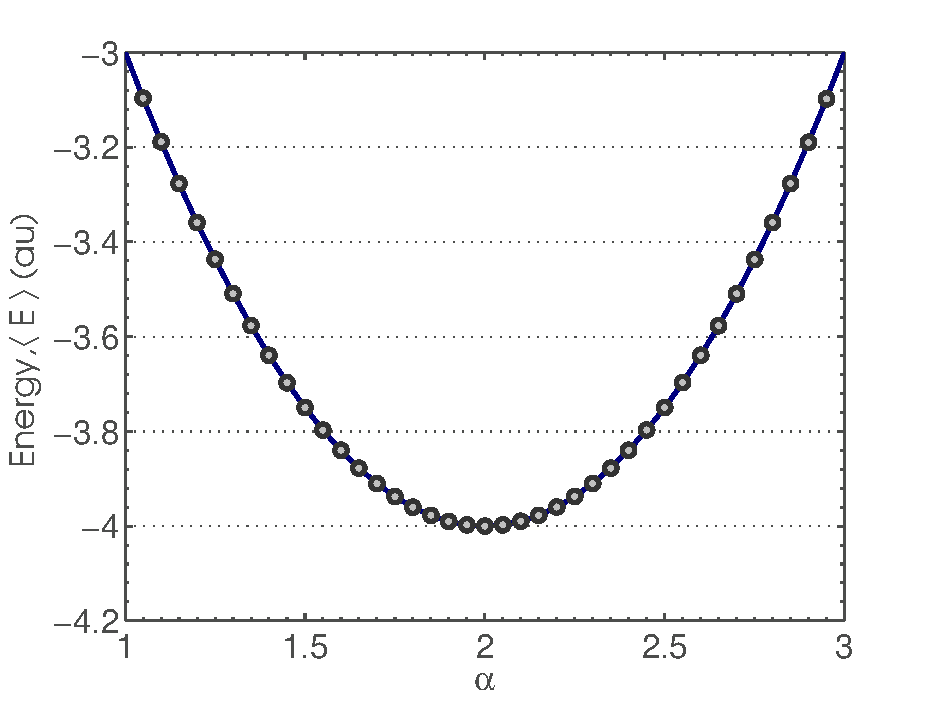
\includegraphics{experimentalData/secondPart/tunningSimulator/alphaStudies/alphaHe}} &
      \resizebox{70mm}{!}{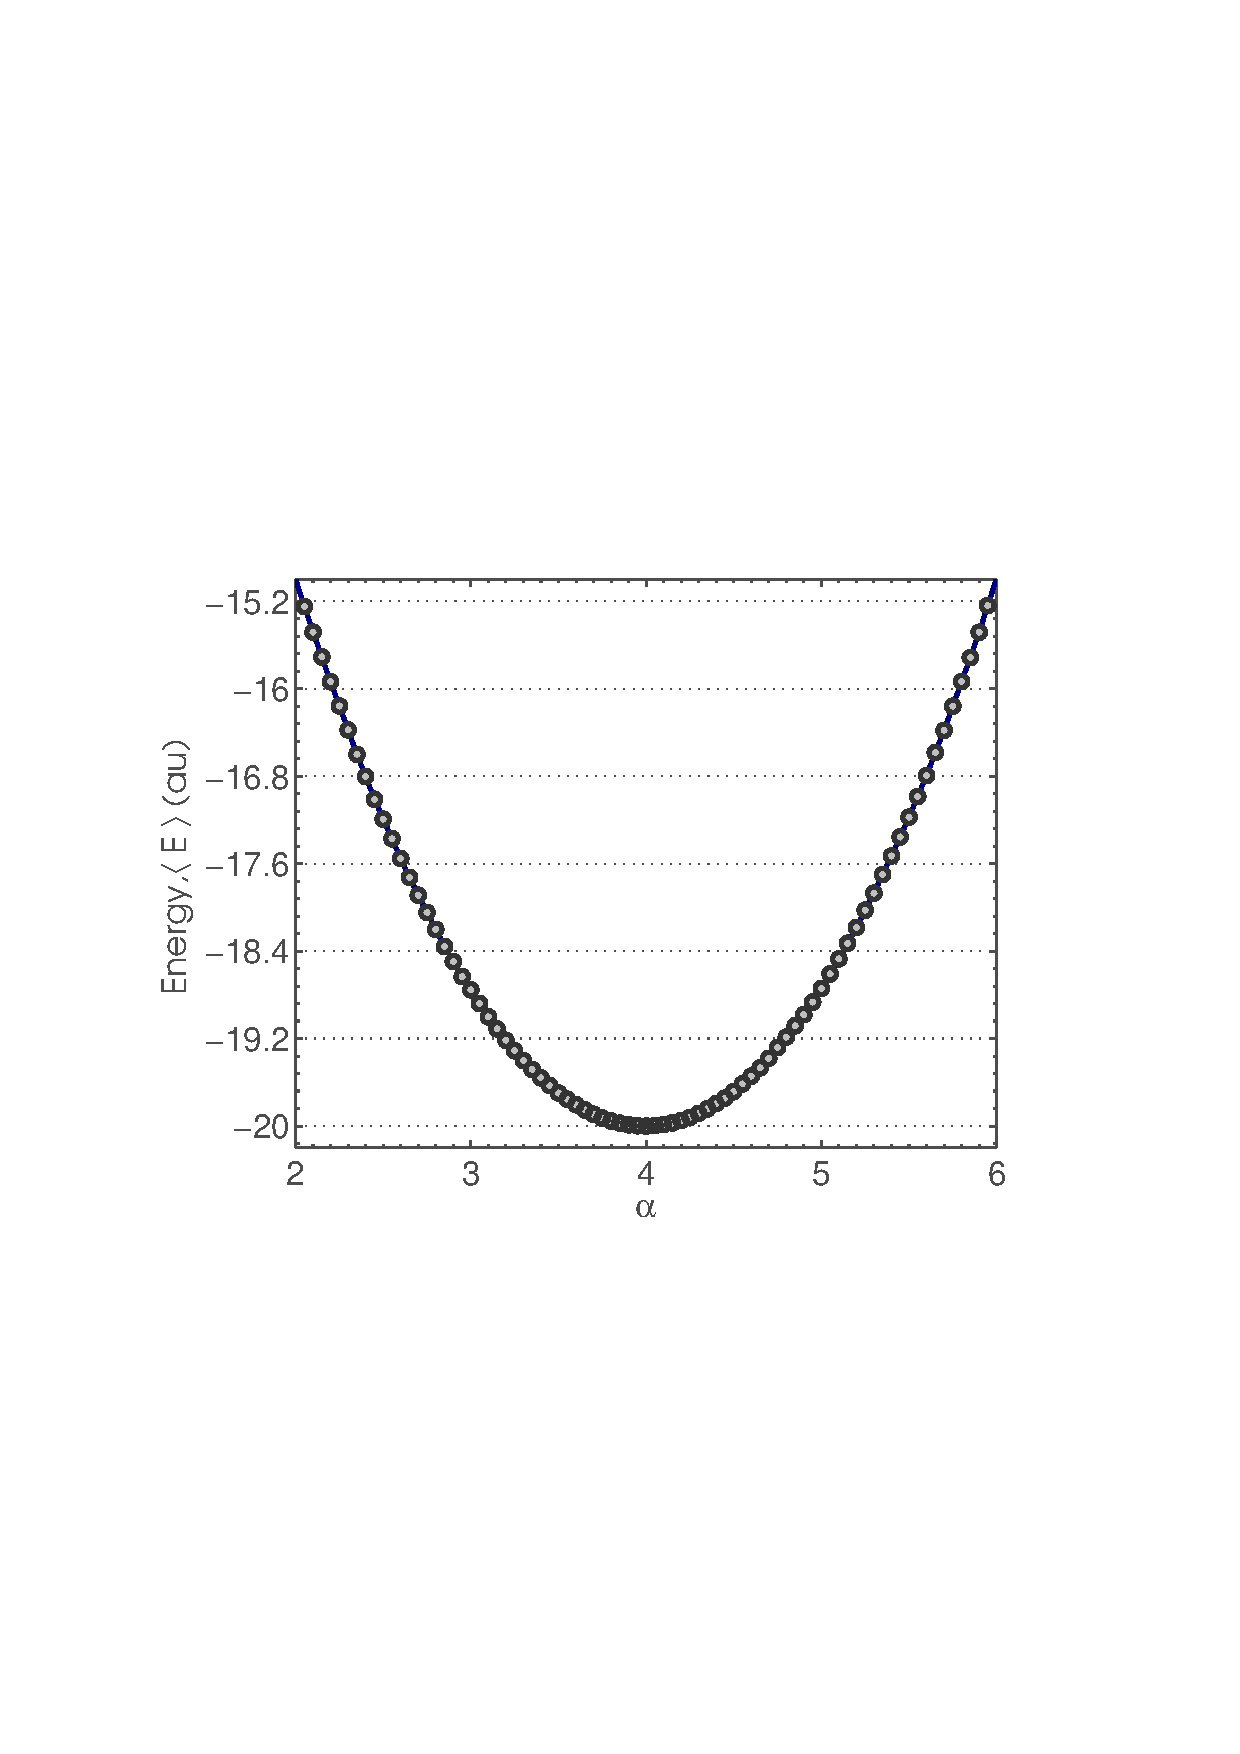
\includegraphics{experimentalData/secondPart/tunningSimulator/alphaStudies/alphaBe}} \\
      \end{tabular}
    \caption{Dependence of the energy on the parameter $\alpha$ for He(left) and Be(right) atoms.}
    \label{alphaHeBe}
  \end{center}
	\end{figure}
	
\noindent
The ground state energies computed in figures \ref{alphaHeBe} to \ref{alpha2DHO2e6e} and table \ref{analyticalEnergyvsAlpha} are in perfect agreement with the analytical values obtained in chapter \ref{cases} section \ref{verification} and fullfil the \emph{zero variance principle} of section \ref{zeroVariancePrinciple}. It is an indication that the Slater determinant part of the simulator works well.
	
	\begin{figure}
    \begin{center}
			 \begin{tabular}{cc}
      \resizebox{75mm}{!}{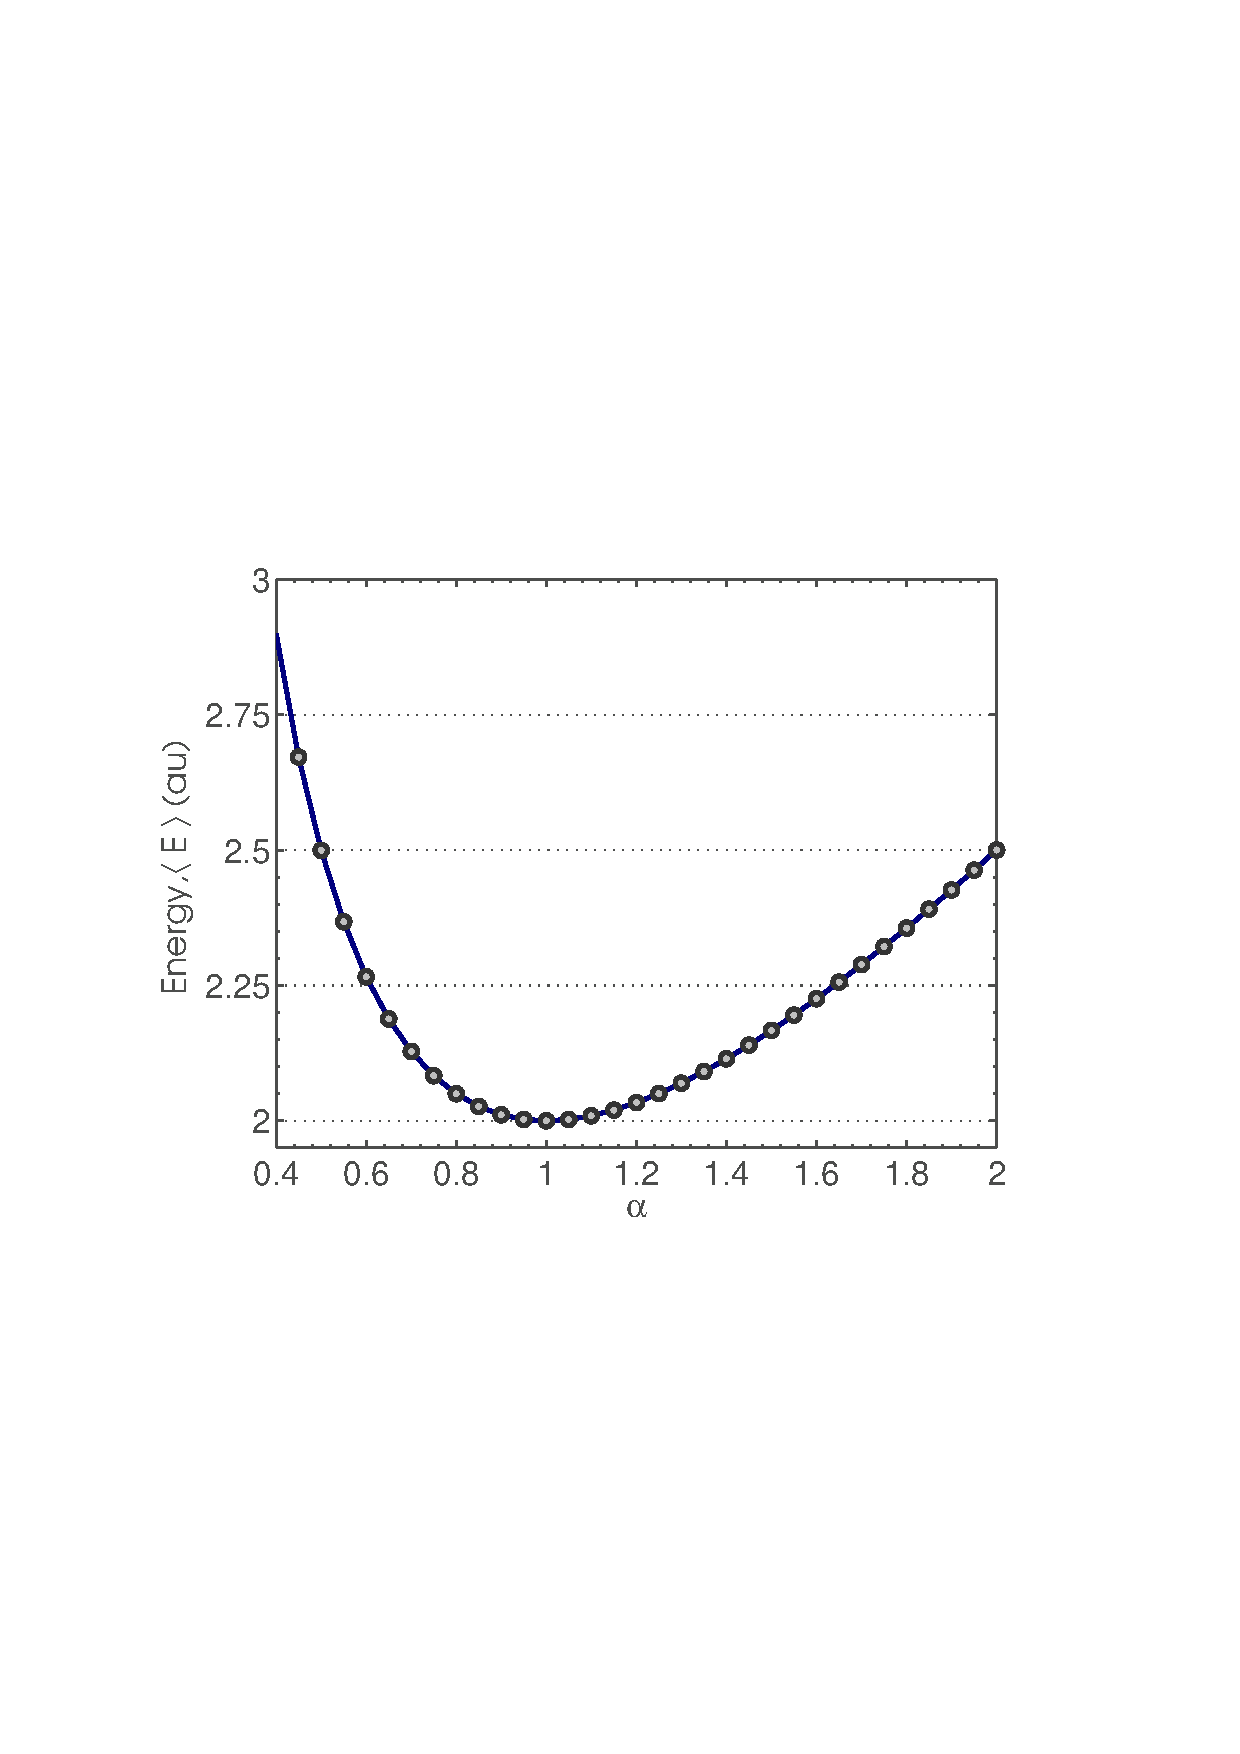
\includegraphics{experimentalData/secondPart/tunningSimulator/alphaStudies/alpha2DHO2e}} &
			\resizebox{75mm}{!}{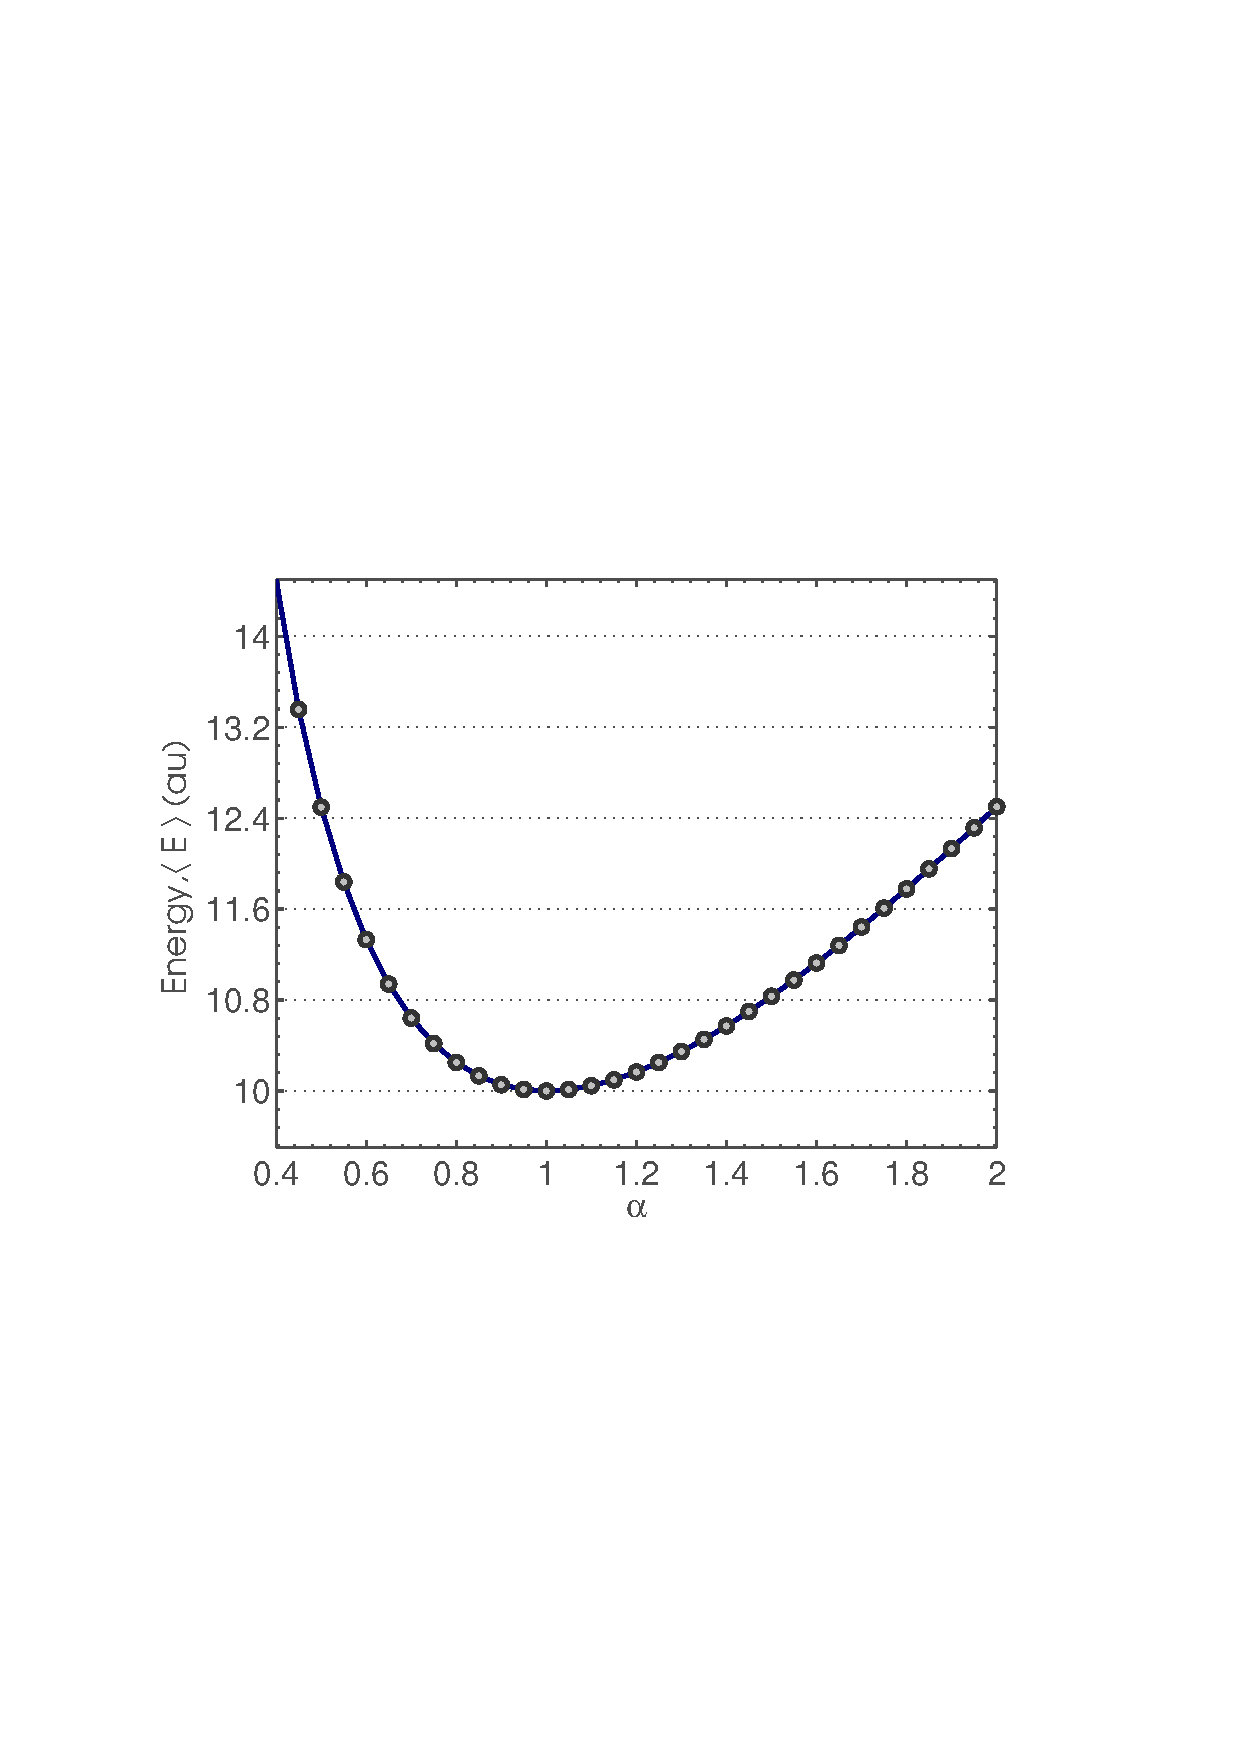
\includegraphics{experimentalData/secondPart/tunningSimulator/alphaStudies/alpha2DHO6e}}\\
			 \end{tabular}
      \caption{Dependence of the energy on the parameter $\alpha$ for a two dimensional harmonic oscillator with two and six electrons electrons, respectively.}
      \label{alpha2DHO2e6e}
    \end{center}
  \end{figure}

	
\begin{table}
\centering
\begin{tabular}{lcc}
\toprule[1pt]
\textbf{System} & \textbf{Ground state energy}, $E$ (au) & $\alpha_{optimal}$ \\
\midrule[1pt]
He  		&  4.0 	&   2.0 \\
Be  		& 20.0 	&   4.0 \\
2DHO2e ($\omega=1.0$)	& 1.0 	&   1.0 \\
2DHO6e ($\omega = 1.0$)	&  10.0  & 	1.0  \\
\bottomrule[1pt]
\end{tabular}\caption{Analytical values of the ground state energy and corresponding variational parameter $\alpha$ computed for the Slater determinant. 2DHO2e stands for two-dimensional harmonic oscillator with two electrons.}
\label{analyticalEnergyvsAlpha}
\end{table}


\subsection{Graphical estimation of the ground state energies}\label{graphicalOptimization}

To examinate the dependence of energy on the variational parameters $\alpha$ and $\beta$ by graphical methods we set the number of Monte Carlo cycles to $1 \times 10^7$ and used 10 \% of equilibration steps with the same $dt$ given in table \ref{expSetUpAlpha}.\\
\\
The estimated values of energy and variational parameters are summarized in table \ref{energiesWithGraphPar}. The relatively big differences observed in energies for atoms and quantum dots are due to the scale length of each of these systems and to the fact that quantum dots do not have a nucleus which the electrons feel. Although these resulst are not exact, they are a good starting point as input parameters for the quasi-Newton method to be used later, and give an insight in which values to expect for energies and optimized variational parameters.\\

\begin{table}[!hbt]
\centering
\begin{tabular}{lcccr}
\toprule[1pt]
\textbf{System} & $\alpha_{optimal}$ & $\beta_{optimal}$ & \textbf{Energy}, $\langle E \rangle$ (au) \\
\midrule[1pt]
He  		&  1.85 	&   0.35 	& $-2.8901 \pm 1.0 \times 10{-4}$ \\
Be  		&  3.96		&   0.09	& $-14.5043 \pm 4.0 \times 10^{-4}$\\
2DQDot2e ($\omega=1.0$)	& 0.98	& 0.41  & $3.0003 \pm 1.2 \times 10^{-5}$ \\
%%%2DQDot6e ($\omega = 1.0$)	& 1.03   & 0.18	& $20.2180 \pm 4.0 \times 10^{-4}$\\
2DQDot6e ($\omega = 1.0$)	& 0.9   & 0.6	& $20.19 \pm 1.2 \times 10^{-4}$\\
\bottomrule[1pt]
\end{tabular}\caption{Values of the ground state (correlated) energy and corresponding variational parameters  $\alpha$ and $\beta$ estimated graphically. The shorthand 2DQDot2e stands for two-dimensional quantum dot with two electrons.}
\label{energiesWithGraphPar}
\end{table}

\noindent
Attempting to optimize in this way is practical just for small systems, where the time of execution for the number of Monte Carlo iterations needed is not critical. Getting an estimate of the variational parameter $\alpha$ in this way is straightforward. For the parameter $\beta$, however, some extra work had to be done. Adjustments of the grids for both $\alpha$ and $\beta$ were necessary to get a good estimate of the last. For systems with more than four electrons, it is not practical because of the computational cost involved.

\begin{figure}[!hbt]
    \begin{center}
      \resizebox{100mm}{!}{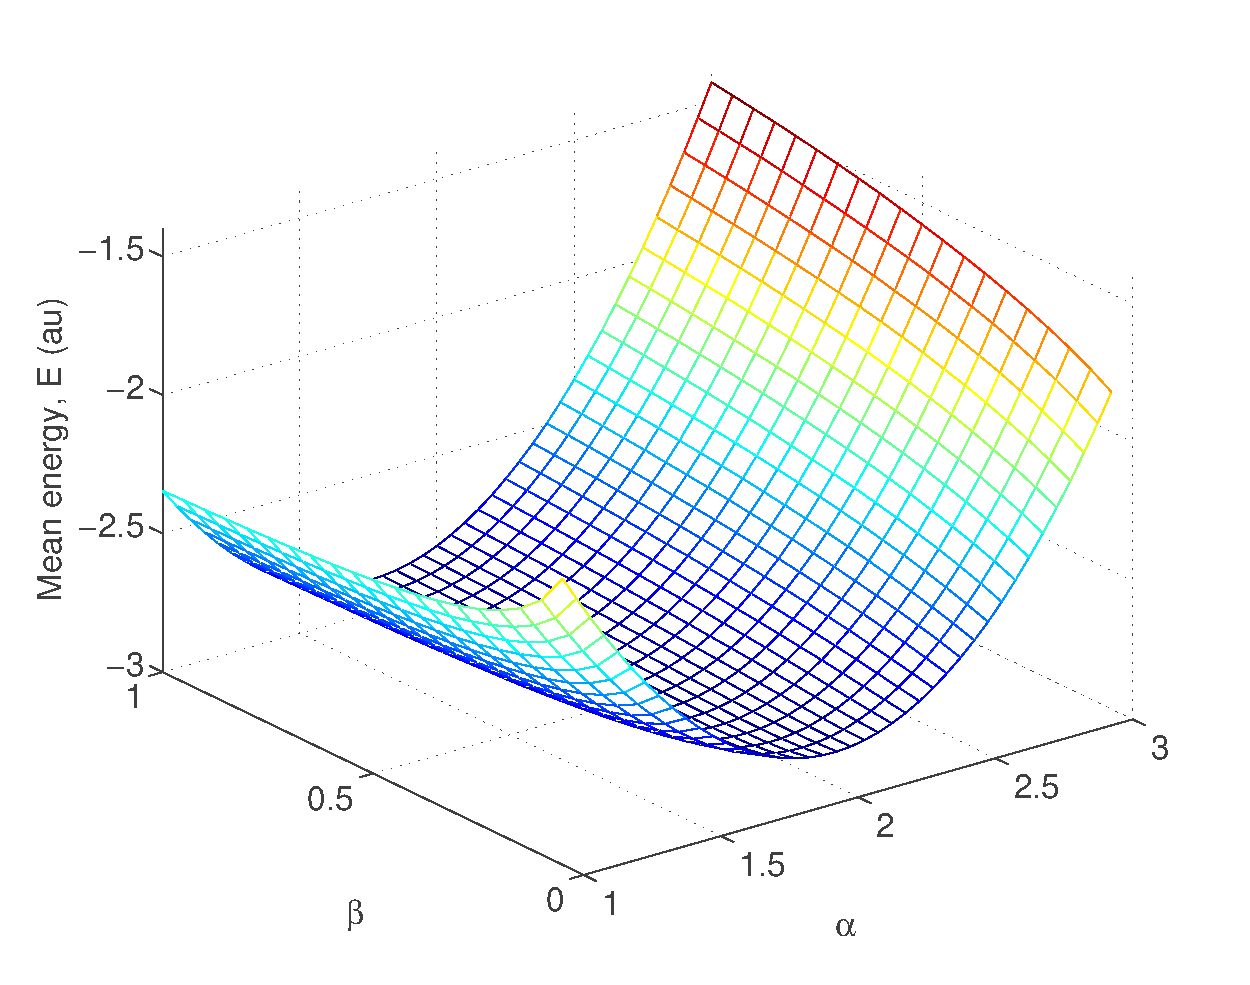
\includegraphics{experimentalData/secondPart/tunningSimulator/He/alphaBetaStudy/plot3DAlphaBetaHe}}%%%%alphaBetaStudies/alphaBetaPlotHe3D}}
      \caption{Dependence of energy on the parameters $\alpha$ and $\beta$ for a He atom. The experimental setup is shown in table \ref{expSetUpAlpha}.}
      \label{alphaBetaHe}
    \end{center}
  \end{figure}

	\begin{figure}[!hbt]
    \begin{center}
			 \begin{tabular}{cc}
      \resizebox{75mm}{!}{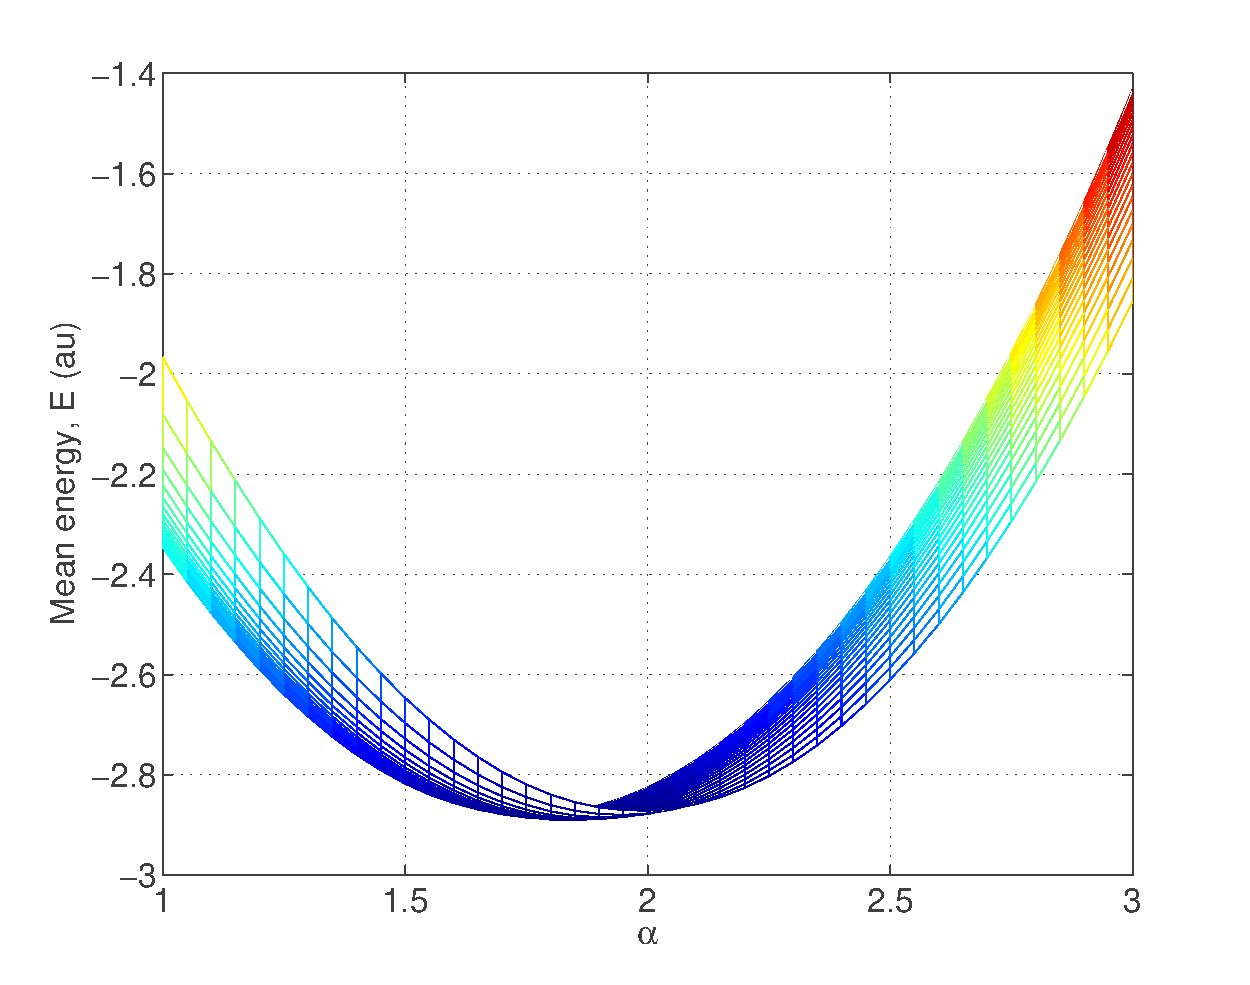
\includegraphics{experimentalData/secondPart/tunningSimulator/He/alphaBetaStudy/zoomAlphaHe}}&%%%alphaBetaStudies/alphaZoomHe}} &
			\resizebox{75mm}{!}{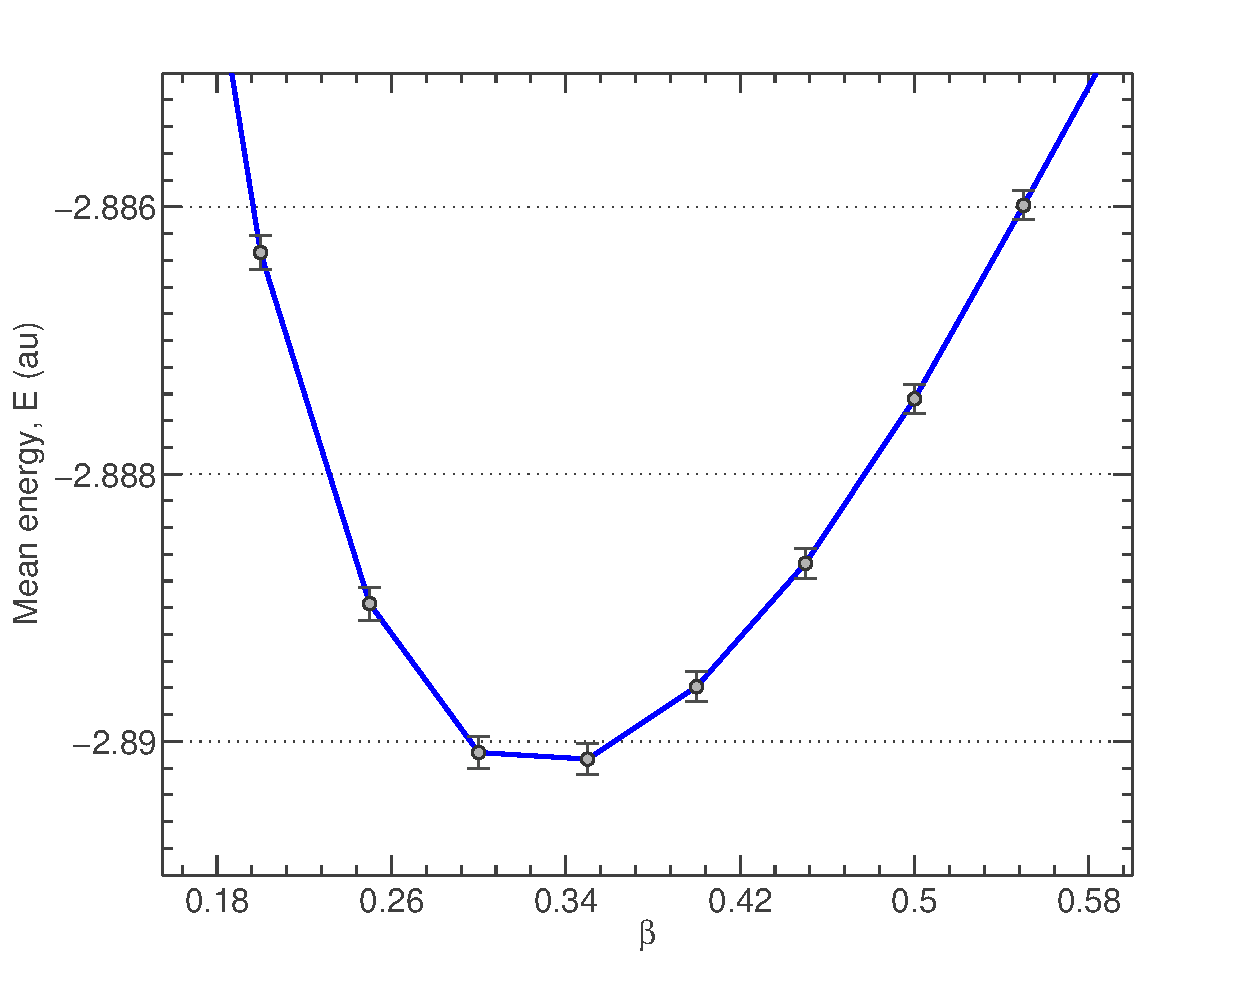
\includegraphics{experimentalData/secondPart/tunningSimulator/He/alphaBetaStudy/minBetaFixedAlphaHe}}\\%%%%alphaBetaStudies/minBetaHeFixedAlpha1_85}}\\
			 \end{tabular}
      \caption{xz-view of $\alpha$ (left) in figure \ref{alphaBetaHe}. To the right we show the dependence of the energy on $\beta$ along the value of $\alpha$ that gives the minimum variational energy for a He atom.  The parameters for these results are shown in table \ref{expSetUpAlpha}.}
      \label{alphaHe}
    \end{center}
  \end{figure}
	
	
	\begin{figure}[!hbt]
    \begin{center}
      \resizebox{100mm}{!}{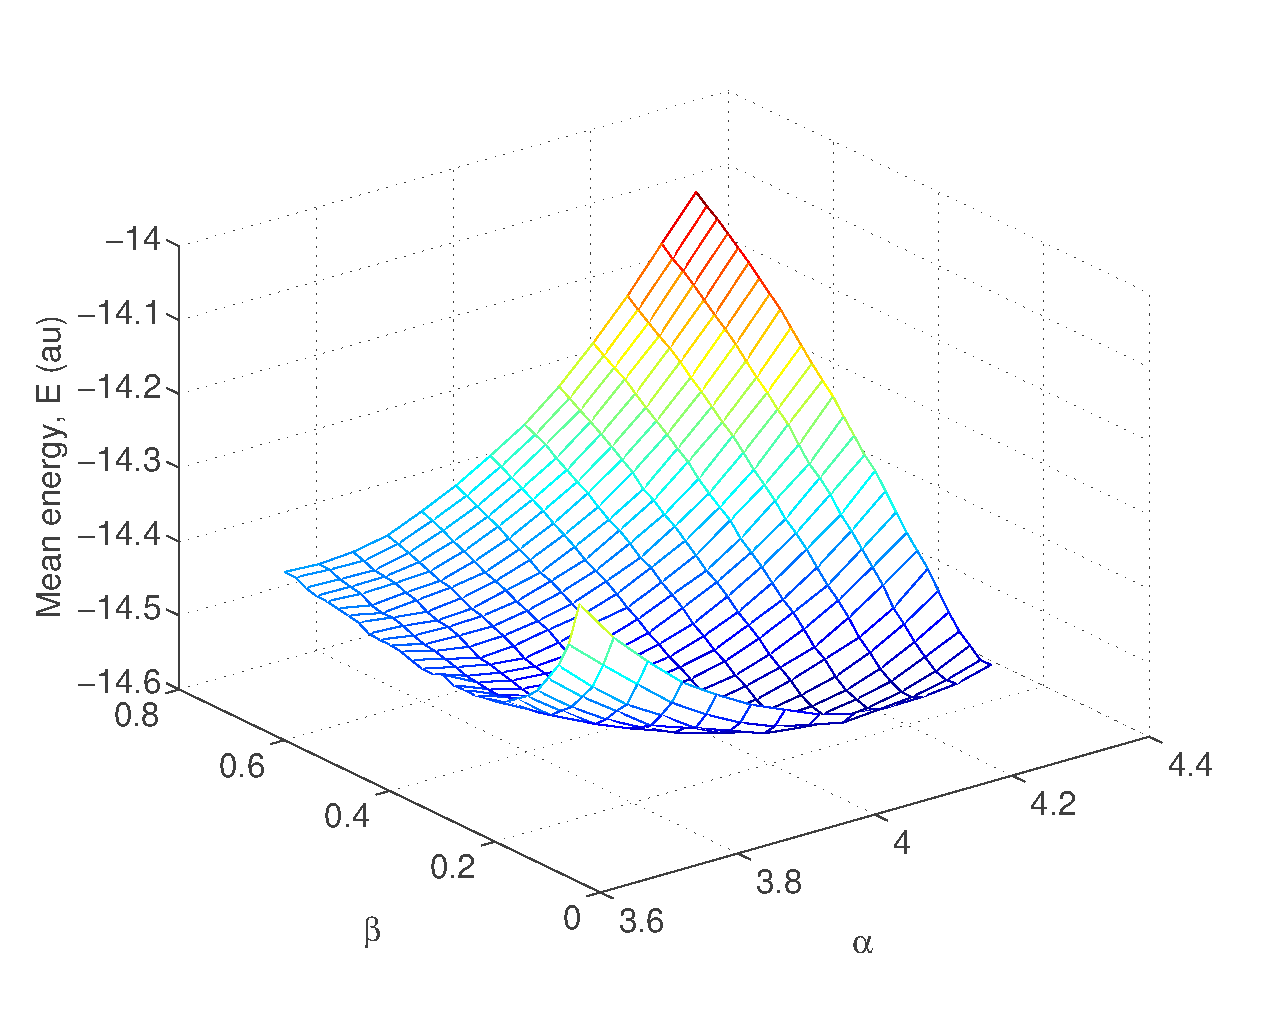
\includegraphics{experimentalData/secondPart/tunningSimulator/Be/alphaBetaStudy/plot3DAlphaBetaBeSim1}}%%%%alphaBetaStudies/alphaBetaPlotHe3D}}
      \caption{Dependence of energy on the parameters $\alpha$ and $\beta$ for a Be atom. The parameters for these results are shown in table \ref{expSetUpAlpha}.}
      \label{alphaBetaBe}
    \end{center}
  \end{figure}


\begin{figure}[!hbt]
    \begin{center}
			 \begin{tabular}{cc}
      \resizebox{75mm}{!}{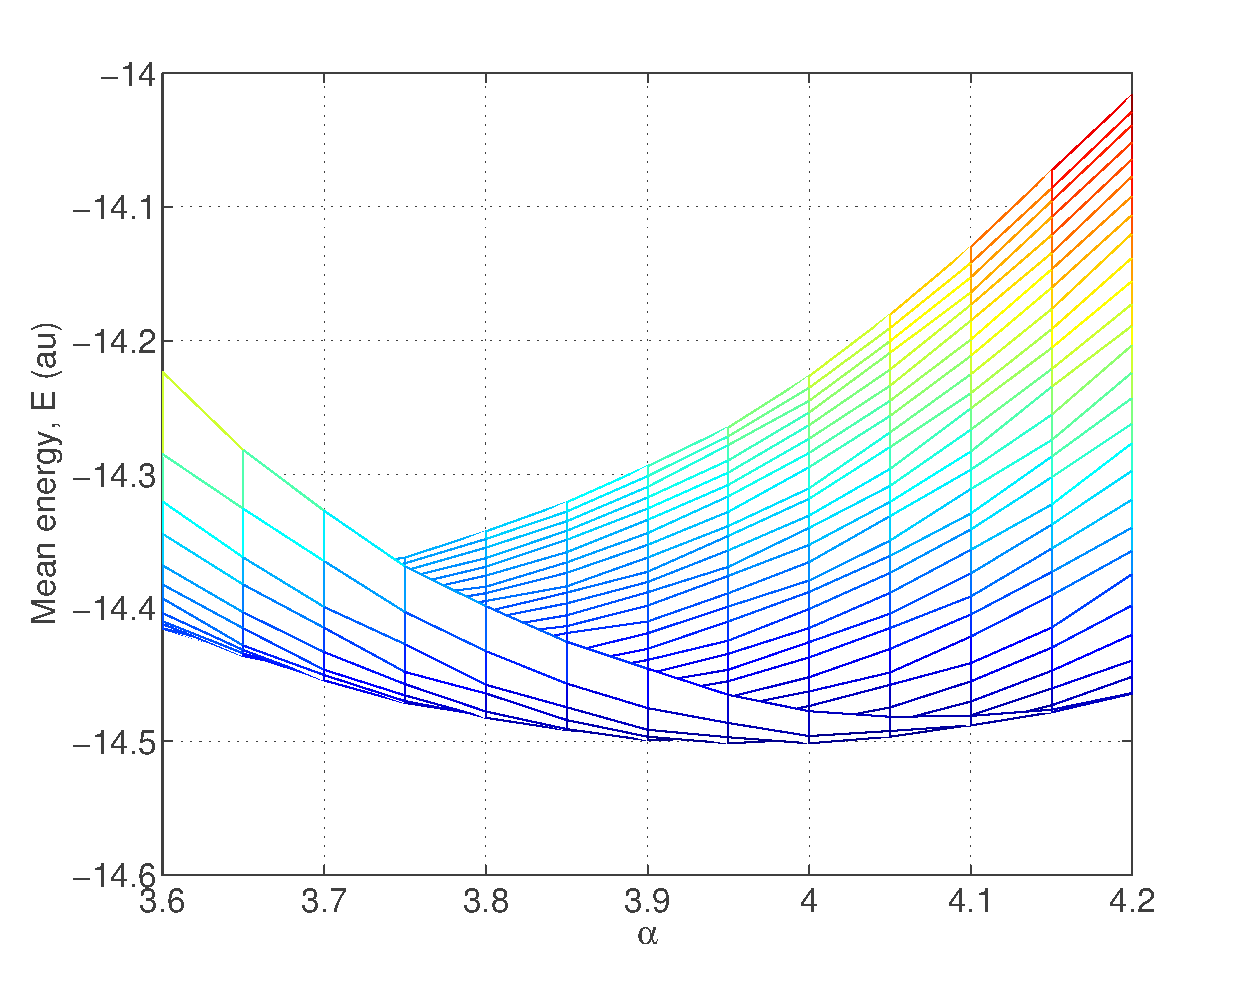
\includegraphics{experimentalData/secondPart/tunningSimulator/Be/alphaBetaStudy/zoomAlphaBeSim1}}&%%%alphaBetaStudies/alphaZoomHe}} &
			\resizebox{75mm}{!}{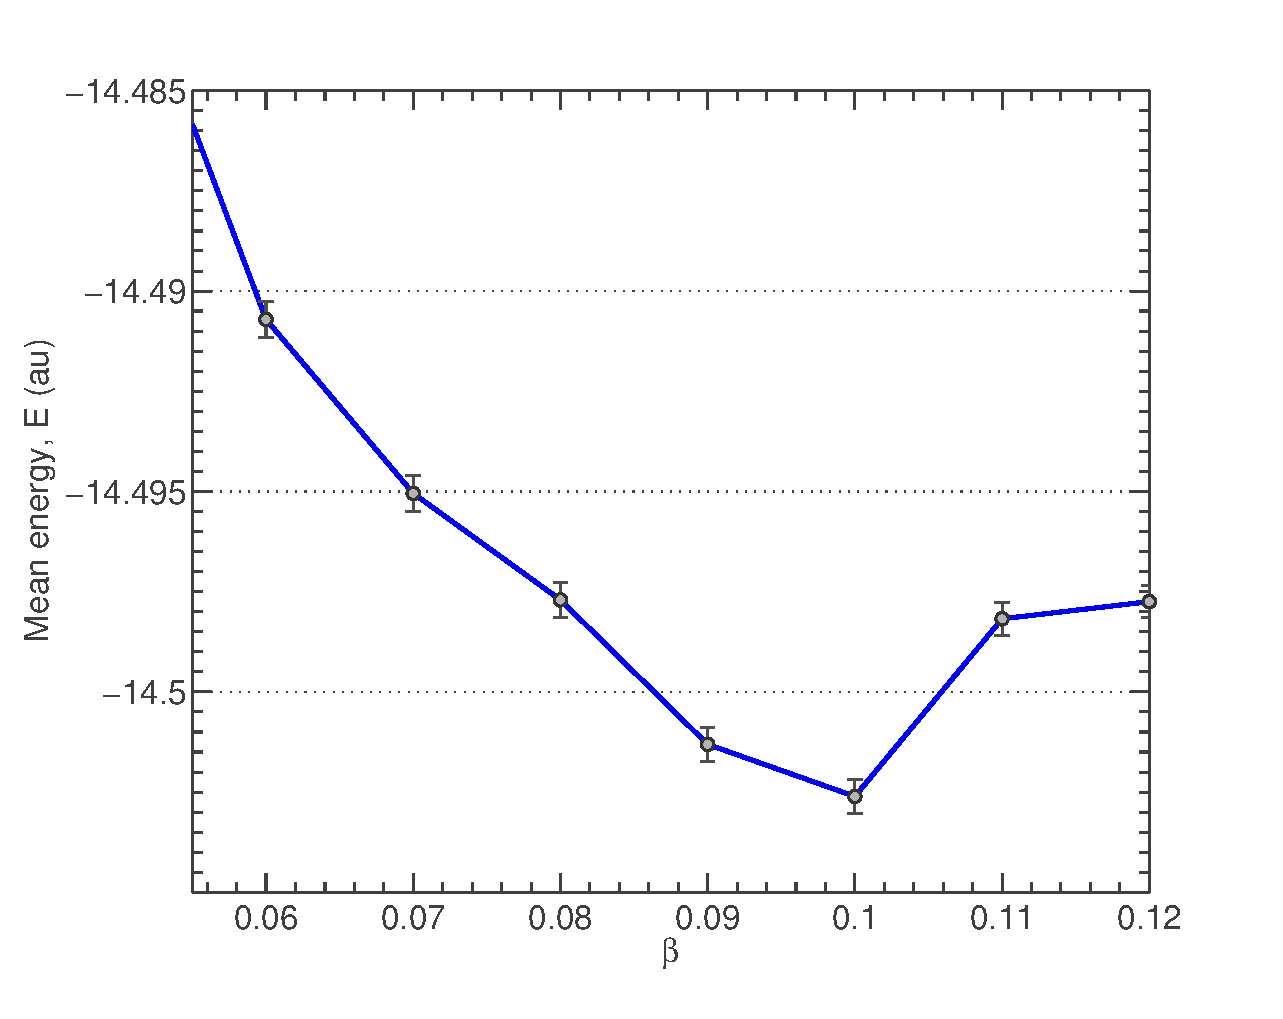
\includegraphics{experimentalData/secondPart/tunningSimulator/Be/alphaBetaStudy/minBetaFixedAlphaBeSim2}}\\%%%%alphaBetaStudies/minBetaHeFixedAlpha1_85}}\\
			 \end{tabular}
      \caption{An xz-view of $\alpha$ (left) in figure \ref{alphaBetaBe}. To the right we show the dependence of the energy on $\beta$ along the value of $\alpha$ which gives the minumum variational energy for a Be atom.  The parameters for these results are shown in table \ref{expSetUpAlpha}.}
      \label{alphaBe}
    \end{center}
  \end{figure}
	
	
	\begin{figure}[!hbt]
    \begin{center}
      \resizebox{100mm}{!}{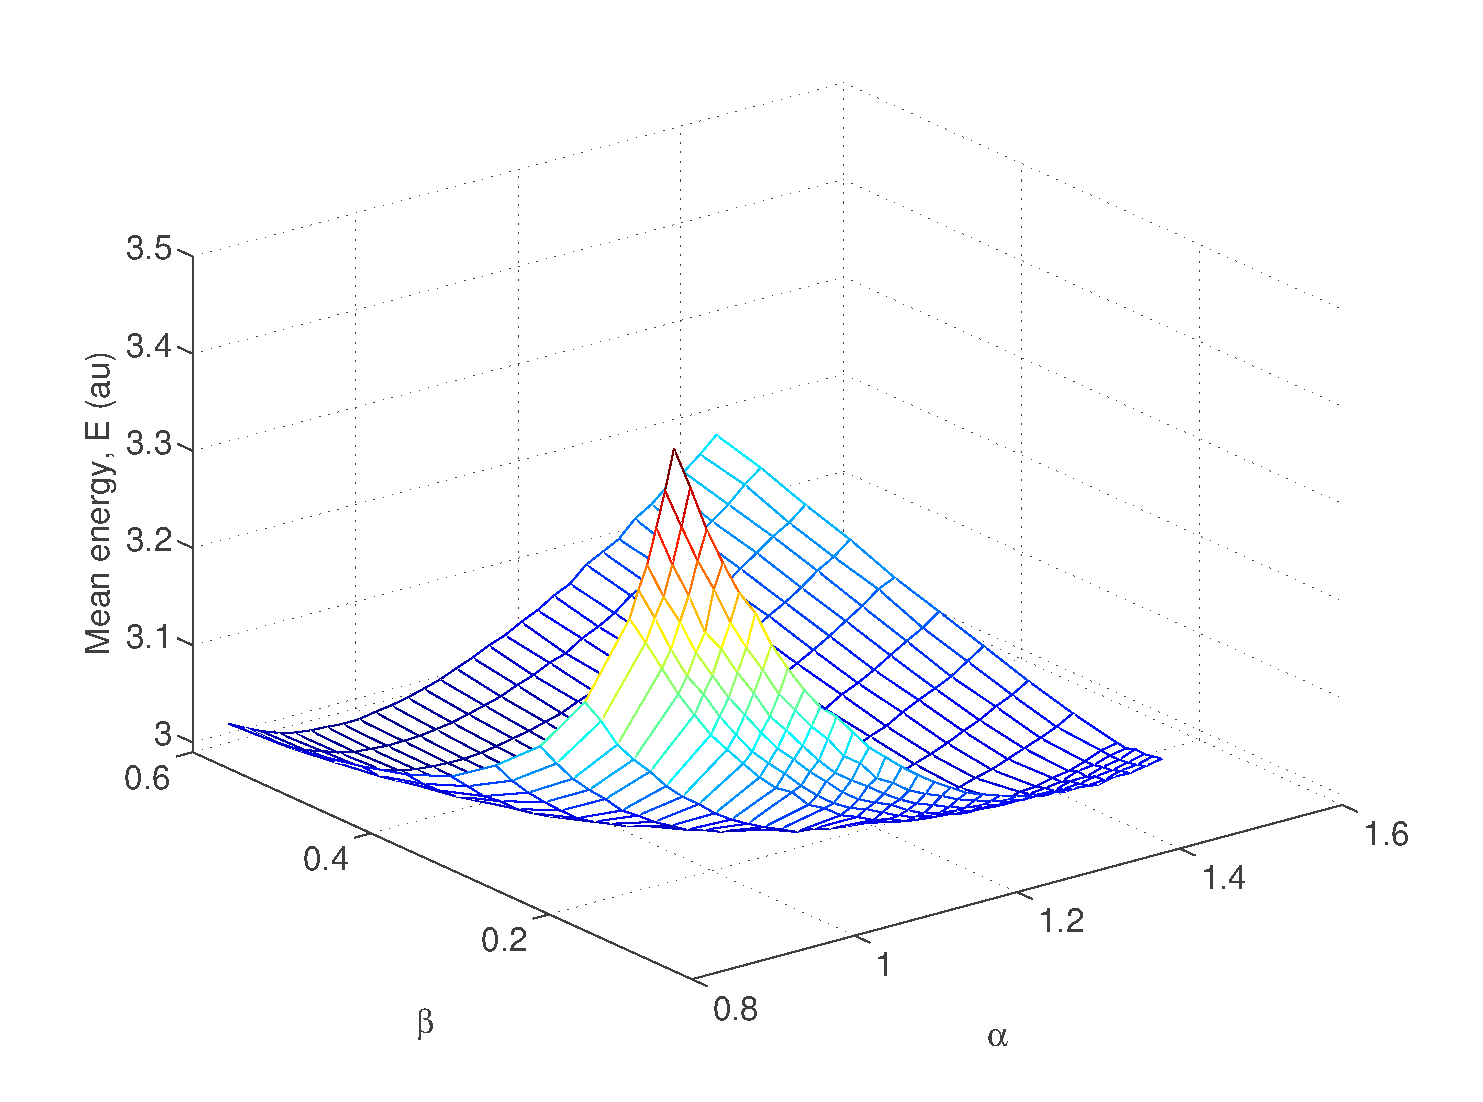
\includegraphics{experimentalData/plots2DQDot2e/plotAlphaBeta2DQDot2e}}
      \caption{Dependence of the energy on the parameters $\alpha$ and $\beta$ for a two dimensional quantum dot with two electrons. The experiment was carried out with $10^7$ Monte Carlo cycles, $10 \%$ equilibration steps and $dt = 0.01$.}
      \label{alphaBeta2DQDot2e}
    \end{center}
  \end{figure}
	
	
	\begin{figure}[!hbt]
    \begin{center}
			 \begin{tabular}{cc}
      \resizebox{75mm}{!}{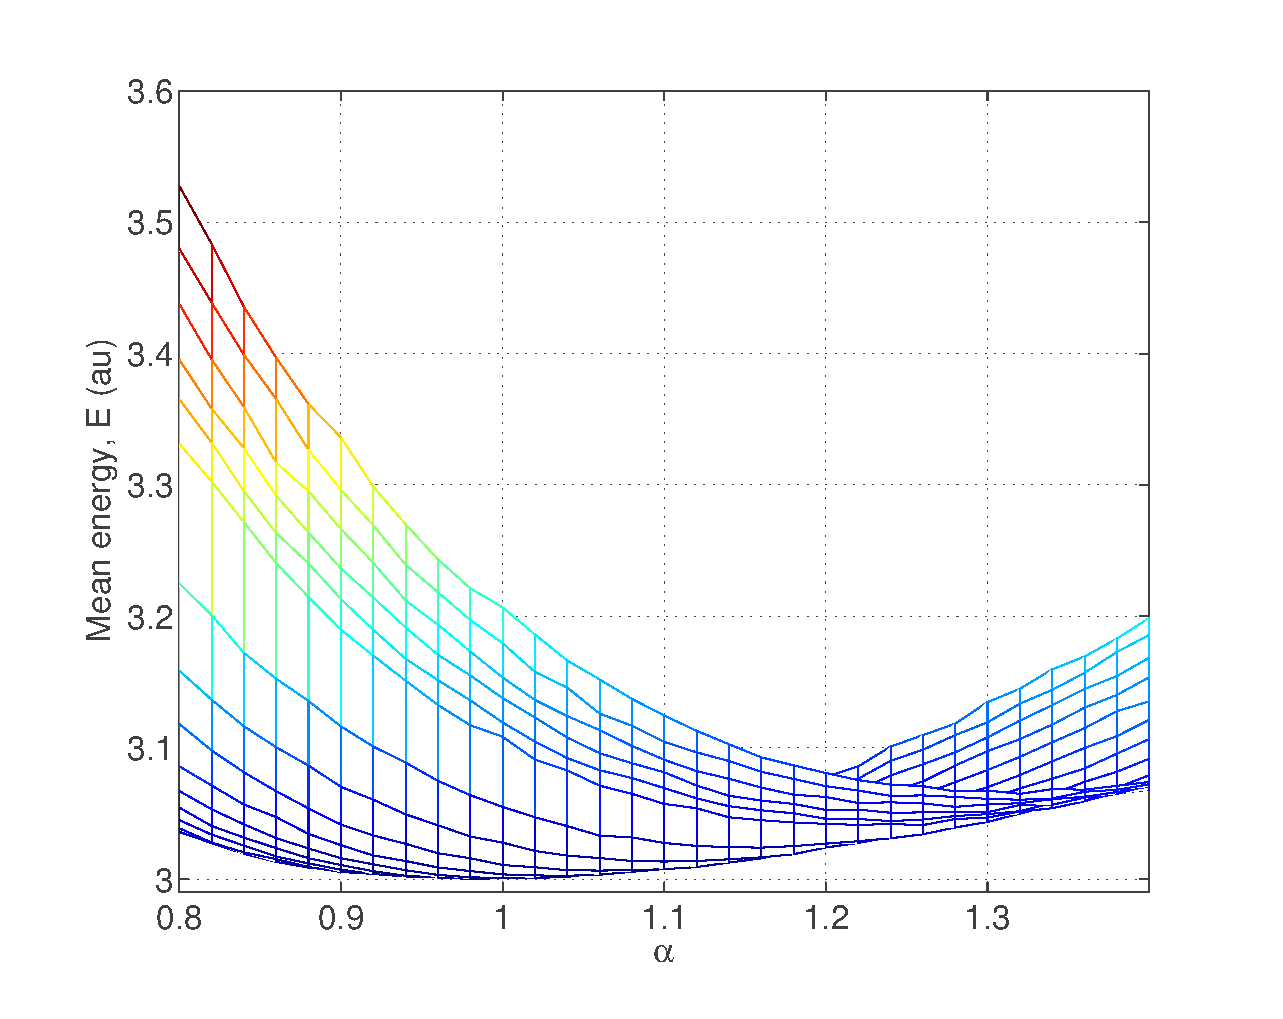
\includegraphics{experimentalData/plots2DQDot2e/zoomAlpha2DQDot2e}} &
			\resizebox{75mm}{!}{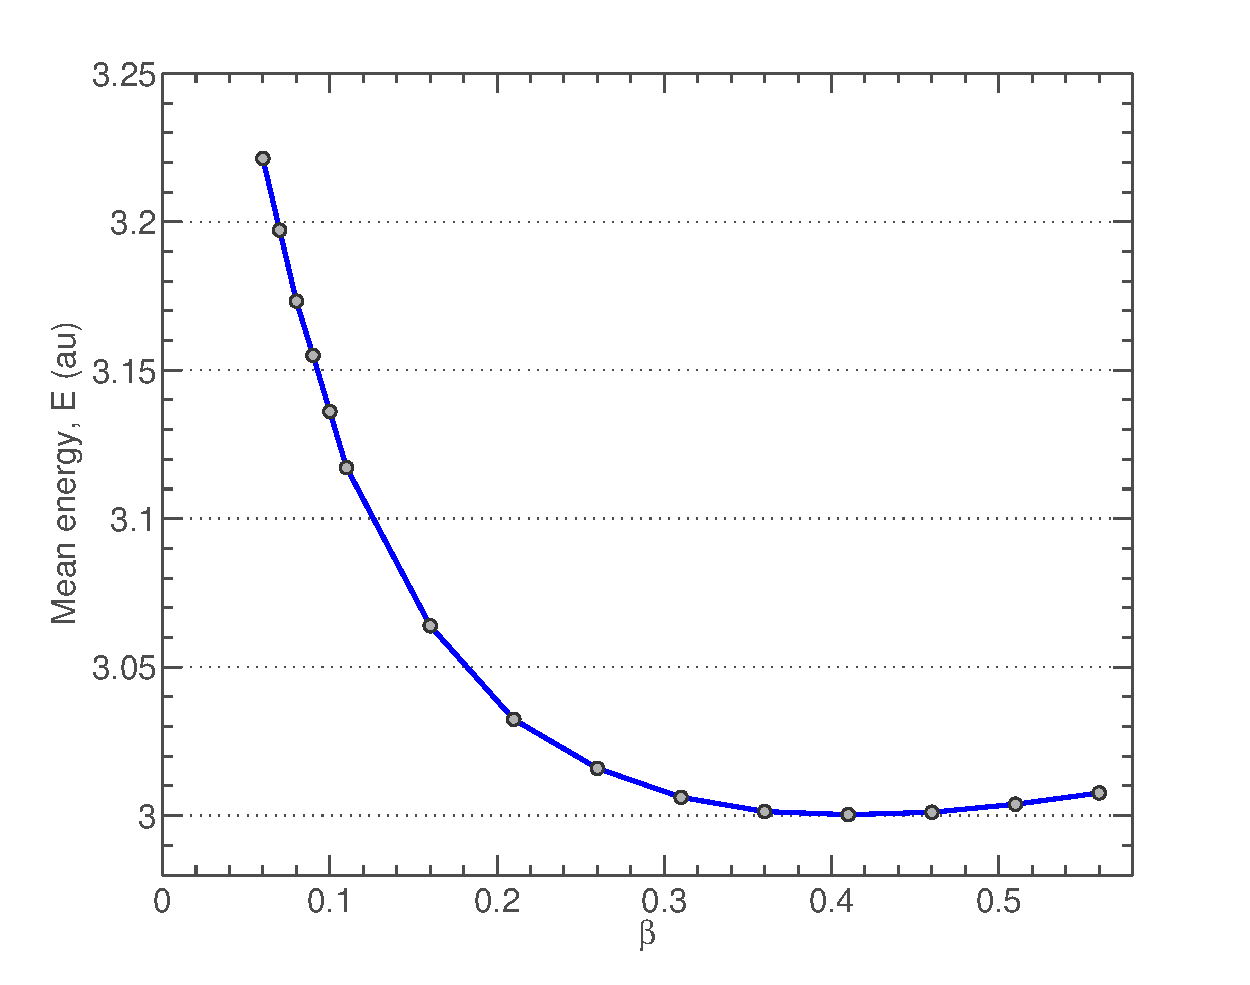
\includegraphics{experimentalData/plots2DQDot2e/zoomBeta2DQDot2e}}\\
			 \end{tabular}
      \caption{An xz-view of $\alpha$ (left) in figure \ref{alphaBeta2DQDot2e}. To the right we show the dependence of the energy on $\beta$ along the value of $\alpha$ that gives the minumum variational energy for a two-dimensional quantum dot with two electrons. The parameters for these results are shown in table \ref{expSetUpAlpha}.}
      \label{alpha2DHO2e}
    \end{center}
  \end{figure}


\begin{figure}[!hbt]
    \begin{center}
      \resizebox{100mm}{!}{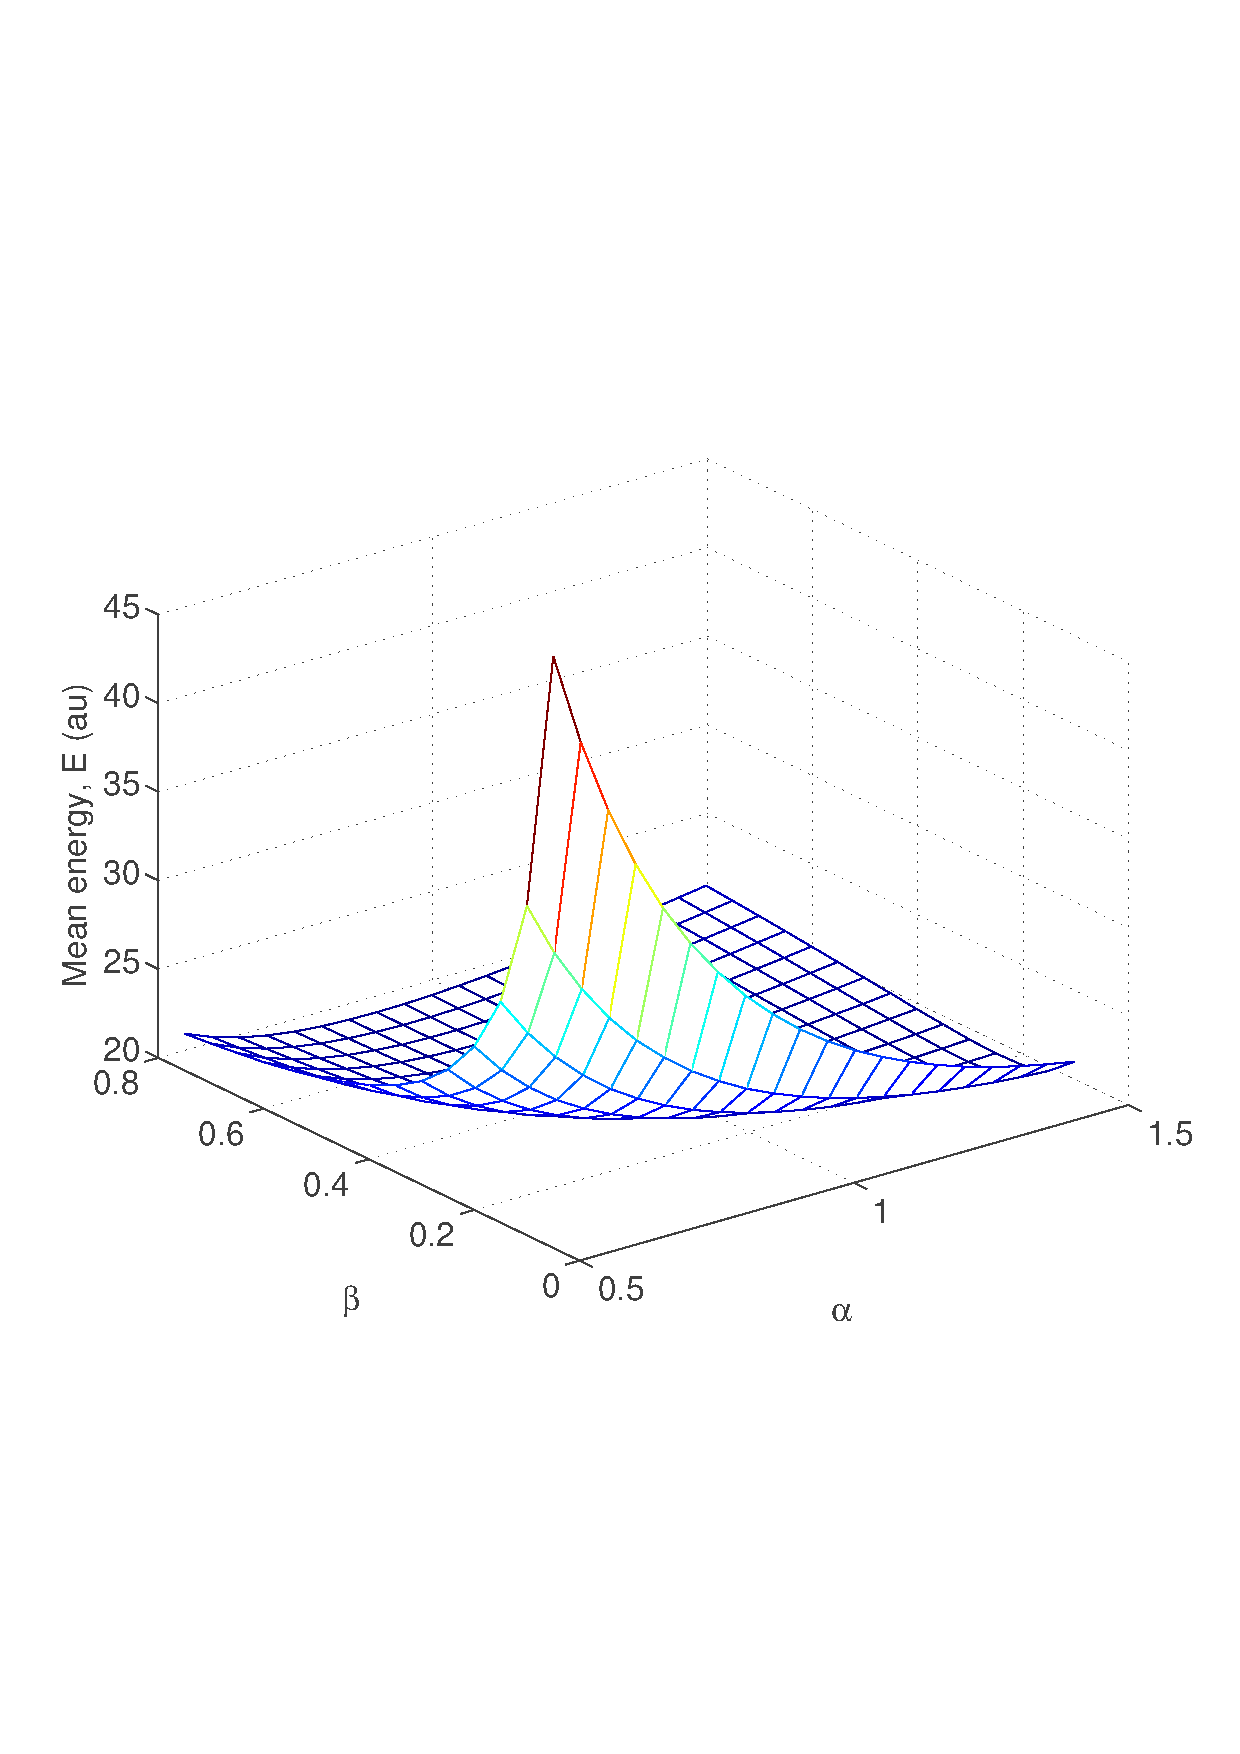
\includegraphics{experimentalData/secondPart/tunningSimulator/2DQDot6e/alphaBeta}}
      \caption{Dependence of energy on the parameters $\alpha$ and $\beta$ for a two dimensional quantum dot with six electrons. The experiment was carried out with $10^7$ Monte Carlo cycles, $10 \%$ equilibration steps and $dt = 0.01$.}
      \label{alphaBeta2DQDot6e}
    \end{center}
  \end{figure}
	
	
	\begin{figure}[!hbt]
    \begin{center}
			 \begin{tabular}{cc}
      \resizebox{75mm}{!}{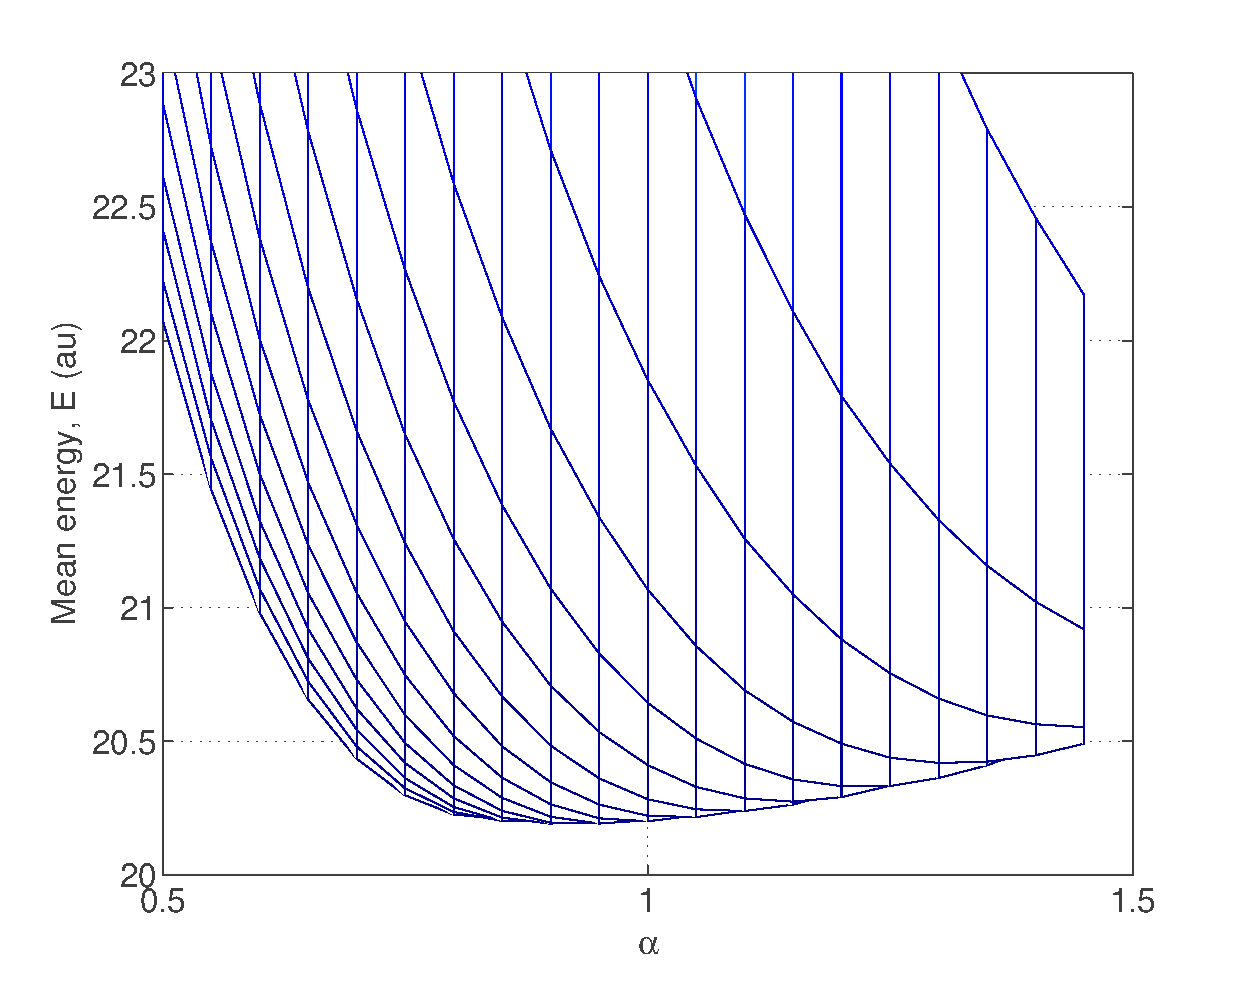
\includegraphics{experimentalData/secondPart/tunningSimulator/2DQDot6e/zoomAlpha}} &
			\resizebox{75mm}{!}{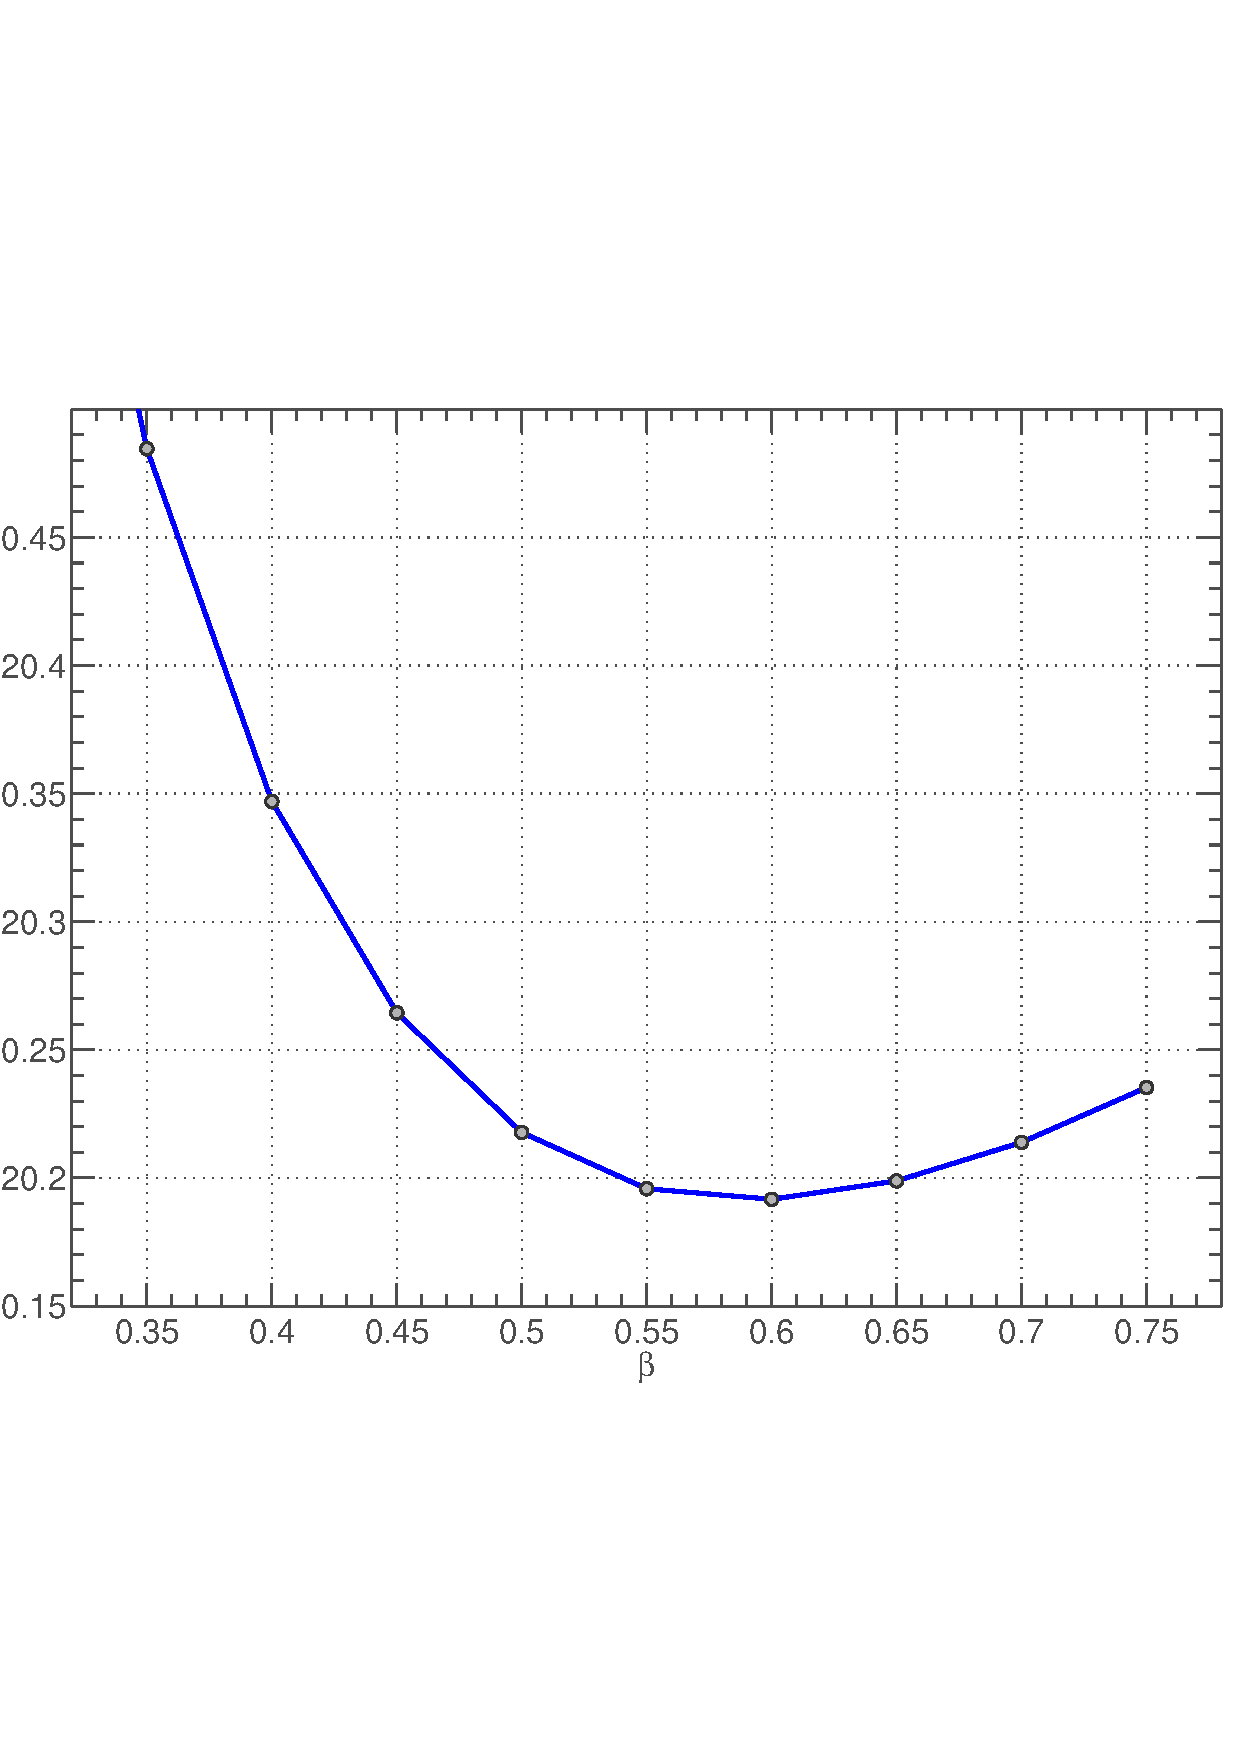
\includegraphics{experimentalData/secondPart/tunningSimulator/2DQDot6e/zoomBeta}}\\
			 \end{tabular}
      \caption{An xz-view of $\alpha$ (left) in figure \ref{alphaBeta2DQDot2e}. To the right we show the dependence of the energy on $\beta$ along the value of $\alpha$ that gives  the minumum variational energy for a two-dimensional quantum dot with six electrons.  The parameters for these results are shown in table \ref{expSetUpAlpha}.}
      \label{alpha2DHO6e}
    \end{center}
  \end{figure}


%%%%%%%%%%%%%%%%%%%%%%%%%%%%%%%%%%%%%%%%%%%%%%%%%%%%%
%%%%%%%%%%%%%%%%%%%%%%%%%%%%%%%%%%%%%%%%%%%%%%%%%%%%%
%%%%%%%%%%%%%%%%%%%%%%%%%%%%%%%%%%%%%%%%%%%%%%%%%%%%%
%%%%%%%%%%%%%%%%%%%%%%%%%%%%%%%%%%%%%%%%%%%%%%%%%%%%%

\section{Optimization of the variational parameters by the quasi-Newton method.}

This section deals with the validation of the quasi-Newton method as an optimization technique for the QVMC algorithm. All the experiments were performed with $1 \times 10^7$ Monte Carlo cycles, 10 \% of equilibration steps in order to reach the most likely state and  a time step $dt = 0.01$ for atoms and $dt = 0.06$ for quantum dots. The time step is used in the importance sampling part.\\
\\
\noindent
The evolution of the variational parameters $\alpha$, $\beta$ and energy during optimization of the trial wave function of He and Be atoms with the quasi-Newton method is shown in figures \ref{quasiNewtonOptHe} and \ref{quasiNewtonOptBe}. In both cases the optimizer makes a big jump during the three first iterations and then stabilizes around the optimal parameters and minimal energy. Table \ref{optizedQuasiNewtonParameters} summarizes the results. In general, these energies are in agreement with the previous computations from section \ref{graphicalOptimization}, confirming that the algorithm suggested in section \ref{effParamDer} for evaluating the numerical derivative of the energy with respect to the variational parameters is correct.\\

\begin{figure}[!hbt]
	\begin{center}
		\resizebox{82mm}{!}{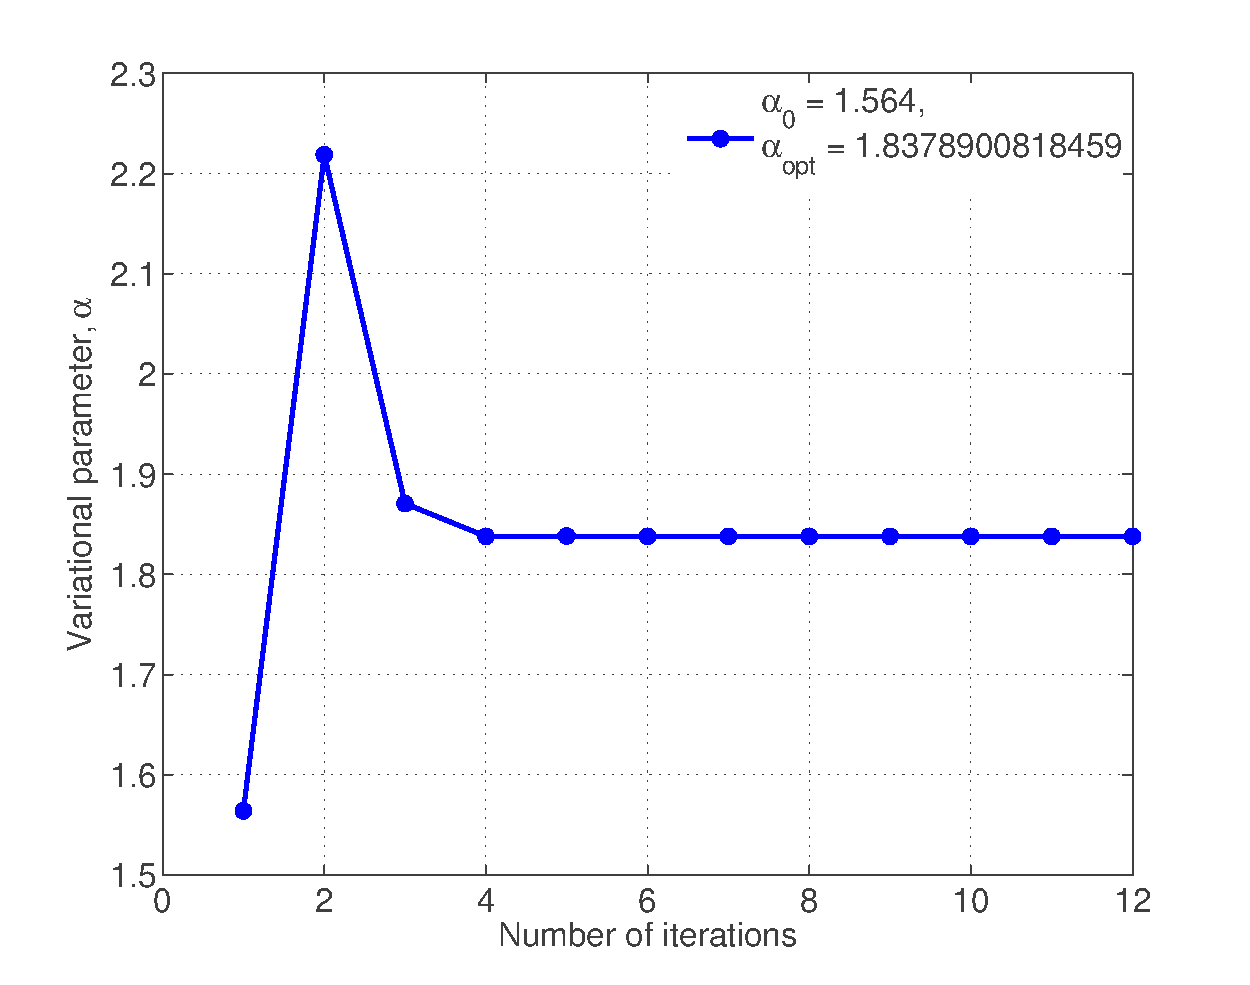
\includegraphics{experimentalData/optimizationWithQuasiNewton/He/plotAlphaEvolHe}}\\
		\resizebox{82mm}{!}{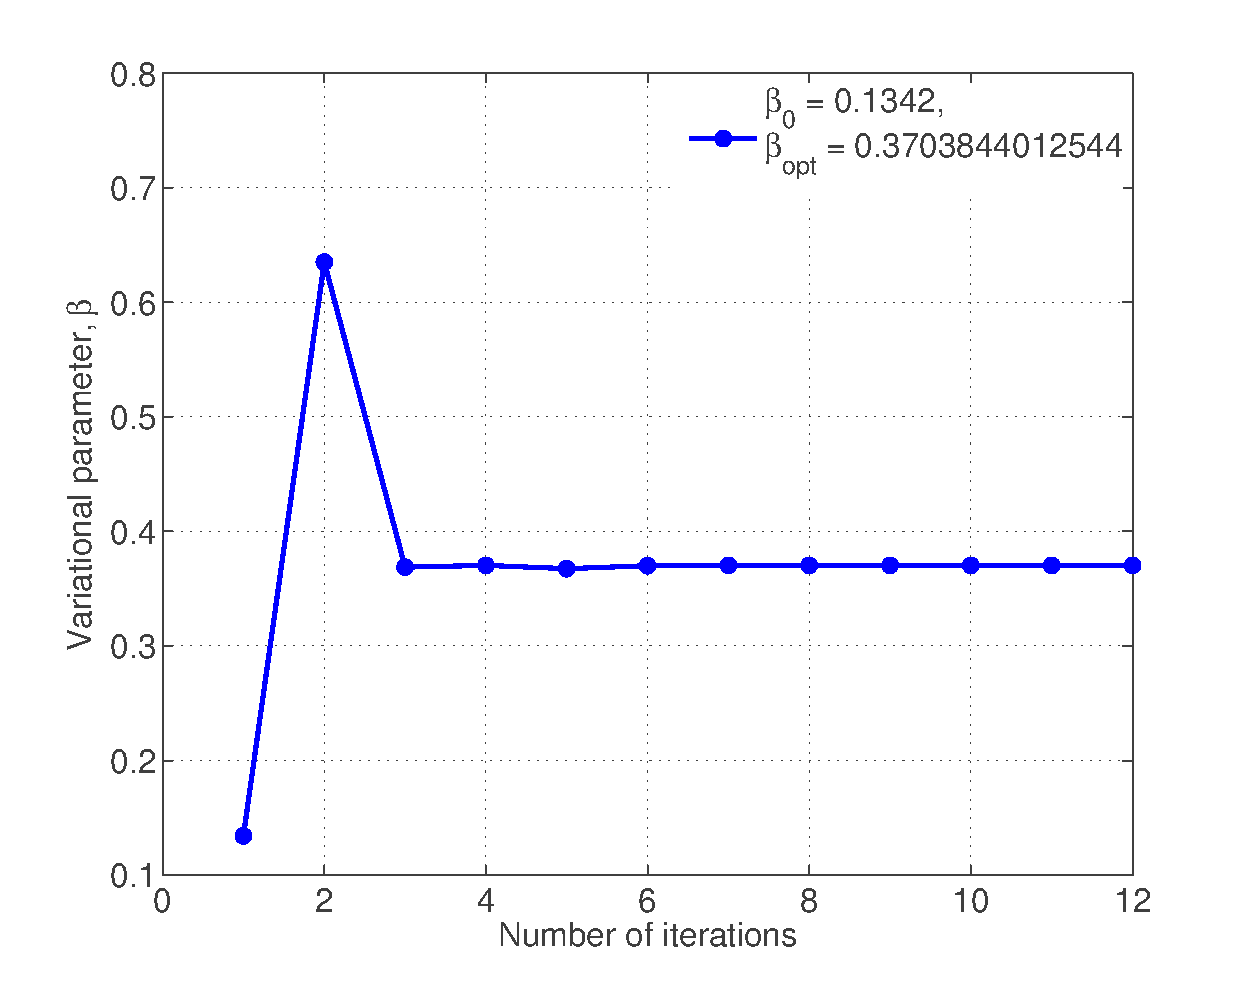
\includegraphics{experimentalData/optimizationWithQuasiNewton/He/plotBetaEvolHe}}\\
		\resizebox{82mm}{!}{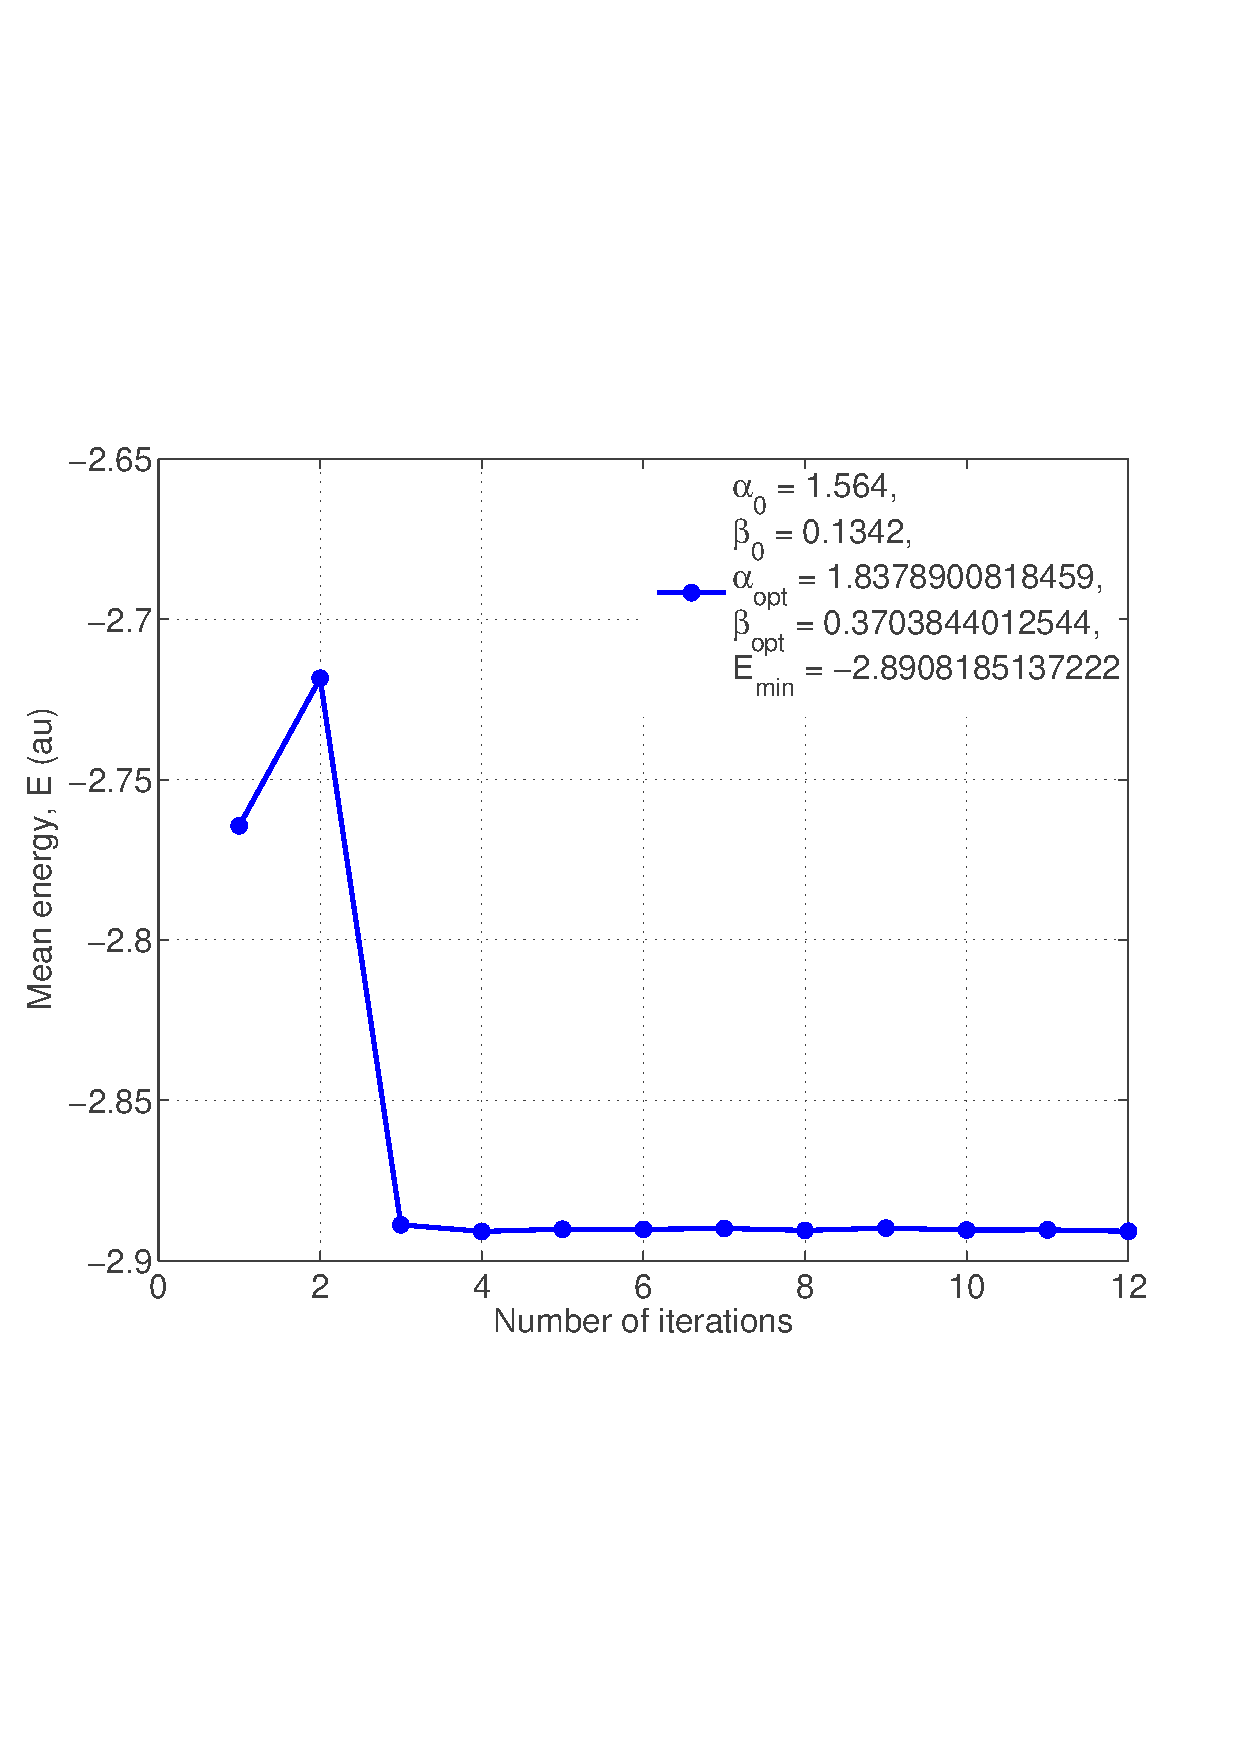
\includegraphics{experimentalData/optimizationWithQuasiNewton/He/plotOptAlphaBetaEnergyHe}}\\
		\caption{Evolution of the variational parameters $\alpha$ and $\beta$ (top), energy (bottom) as a function of the number of iterations during the optimization phase with the quasi-Newton method of the trial wave function of He atom. The experiment was carried out with $10^7$ Monte Carlo cycles and $10 \%$ equilibration steps in four nodes.}
		\label{quasiNewtonOptHe}
	\end{center}
\end{figure}

\begin{figure}[!hbt]
	\begin{center}
		\resizebox{82mm}{!}{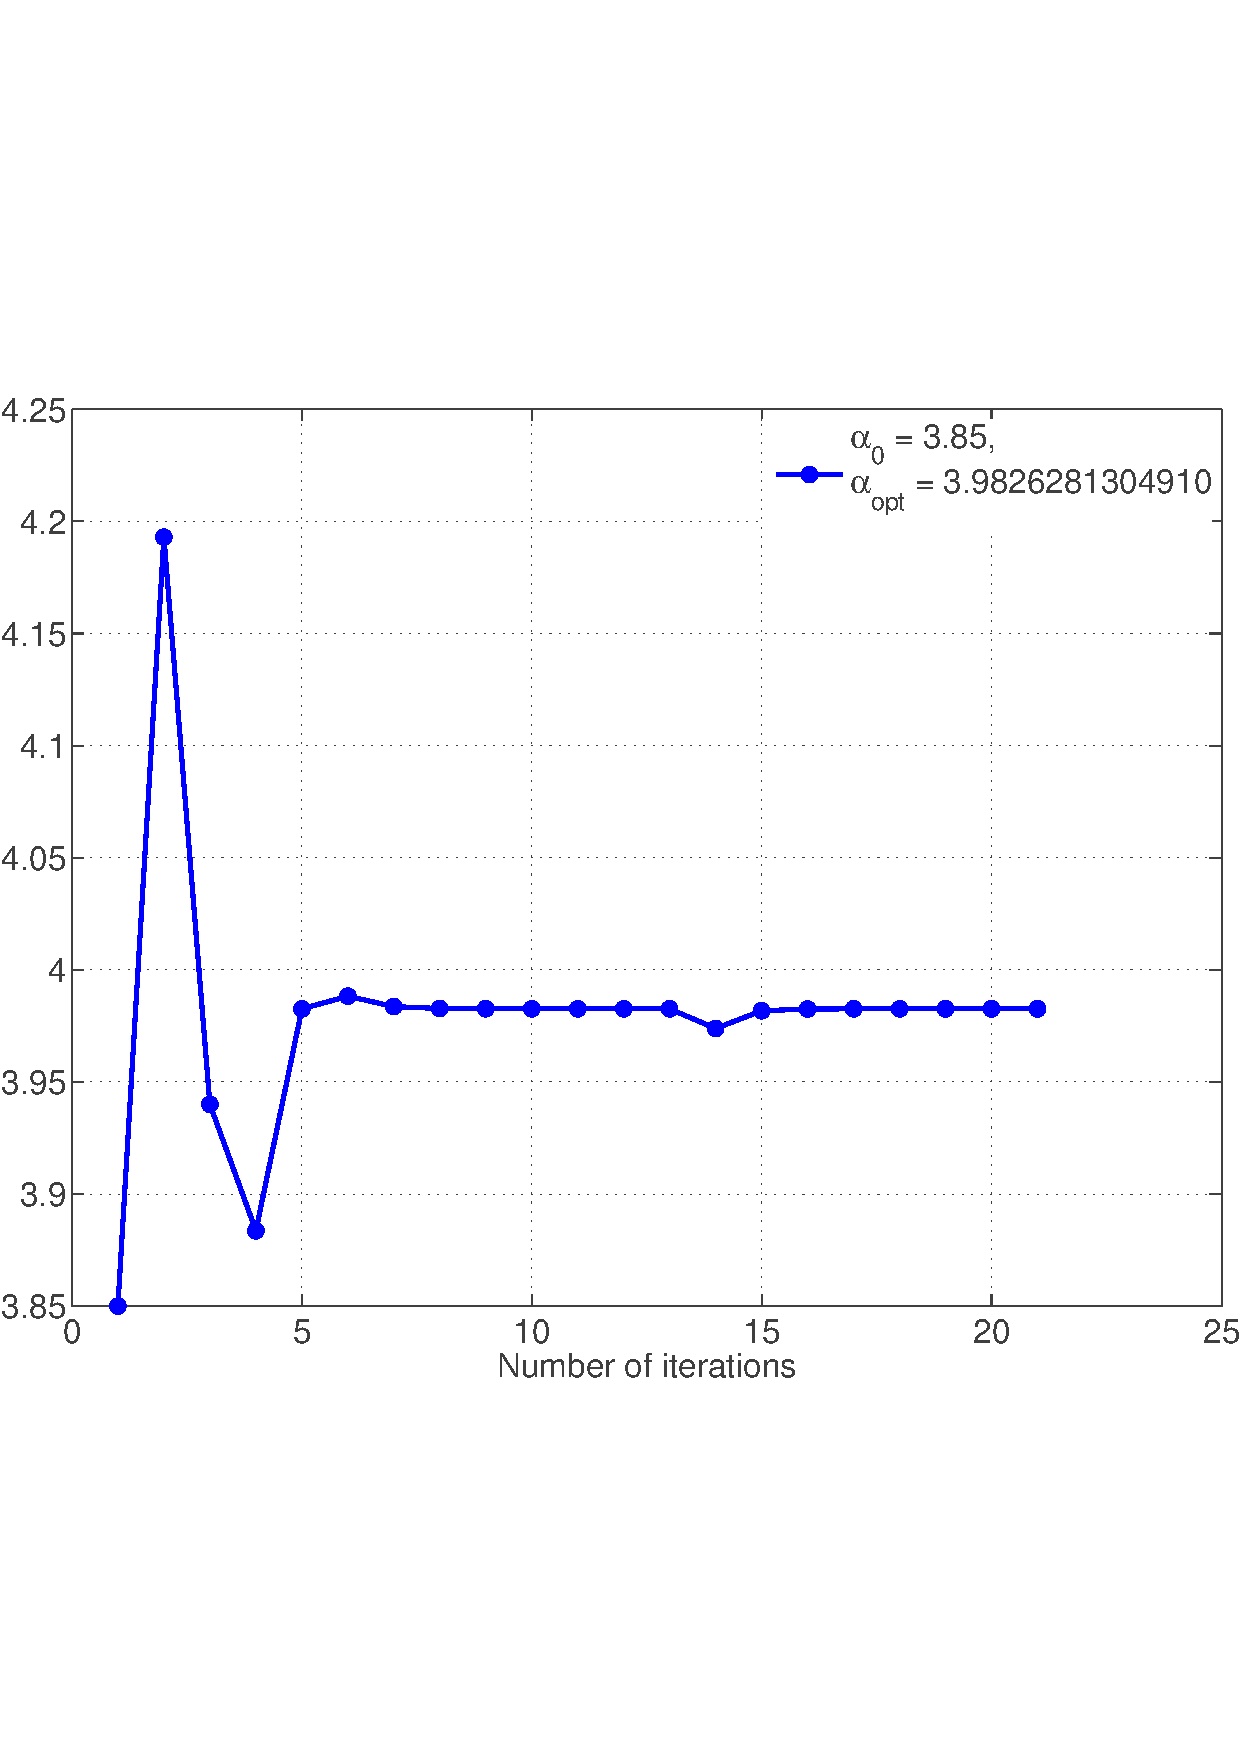
\includegraphics{experimentalData/optimizationWithQuasiNewton/Be/evolAlphaBeOpt}}\\
		\resizebox{82mm}{!}{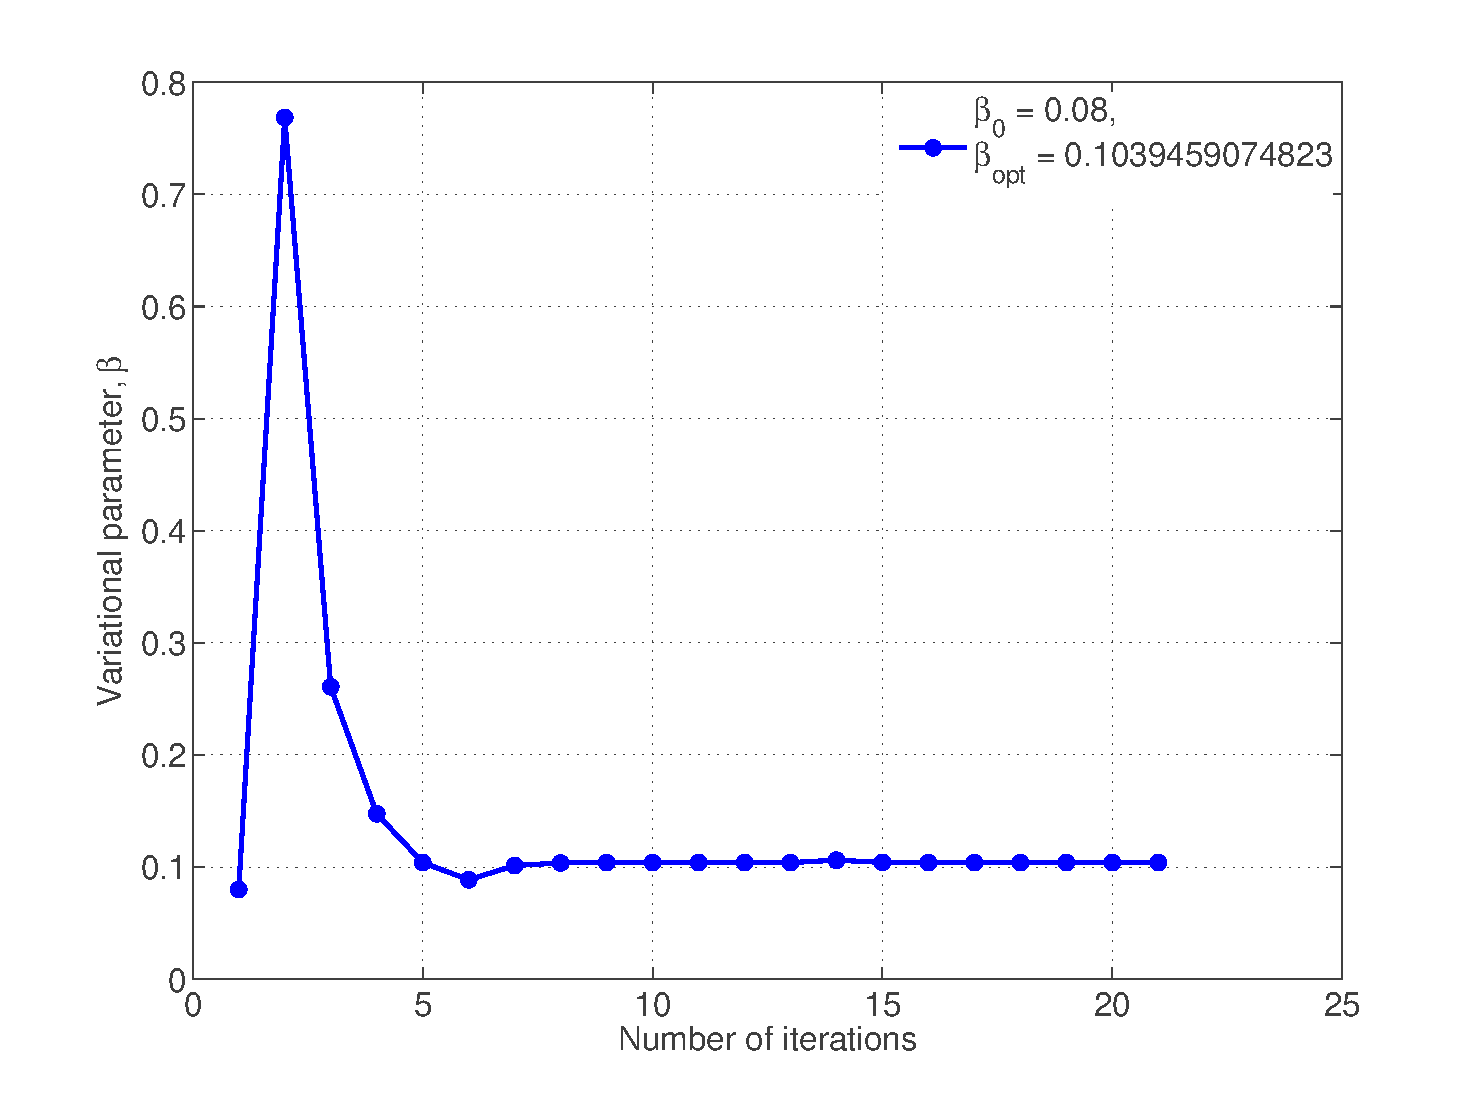
\includegraphics{experimentalData/optimizationWithQuasiNewton/Be/evolBetaBeOpt}}\\
		\resizebox{82mm}{!}{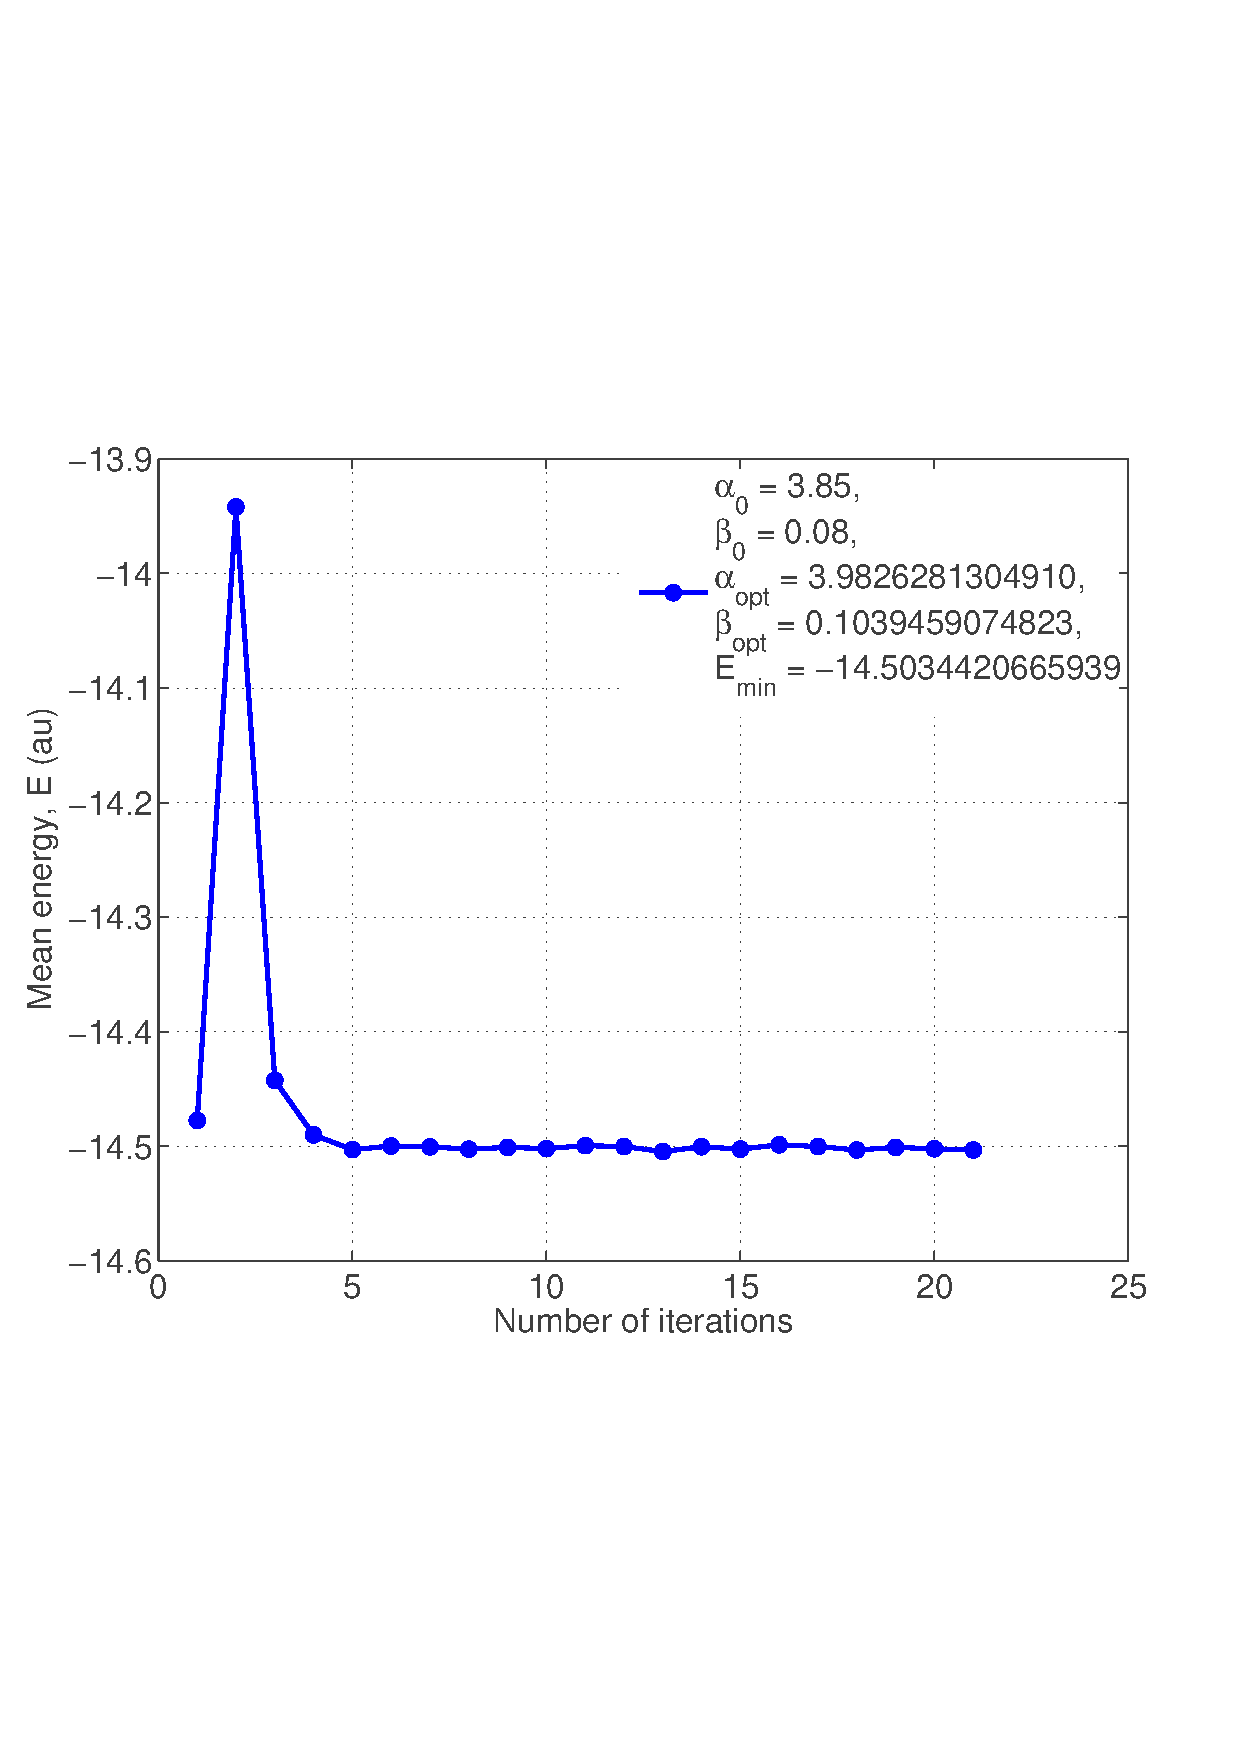
\includegraphics{experimentalData/optimizationWithQuasiNewton/Be/plotEnergyOptimizationBe}}\\
		\caption{Evolution of the variational parameters $\alpha$ and $\beta$ (top), energy (bottom) as a function of the number of iterations during the optimization stage with the quasi-Newton method of the trial wave function of Be atom. The experiment was carried out with $10^7$ Monte Carlo cycles and $10 \%$ equilibration steps in four nodes.}
		\label{quasiNewtonOptBe}
	\end{center}
\end{figure}

\noindent
For quantum dots, the optimization of the trial wave function failed, becacuse it is almost constant with respect to the variational parameter $\beta$ in the region where the minimum is supposed to be located. Therefore, the approximated gradient computed in the quasi-Newton algorithm becomes zero or is very small for these points.  This optimization method uses the gradient to build up the curvature information at each iteration to formulate a quadratic model problem, which explains the success when optimizing wave functions of atoms. In the following we use the variational parameters $\alpha$ and $\beta$ reported by Albrigtsen \cite{Albrigtsen}.\\
\\
Deterministic methods are, in general, not suitable for problems affected by noise. They are either unable to reach an optimum or reach a false one \cite{Harju1997}. A better option is the so called Stochastic Gradient Approximation (SGA). It is a probabilistic iterative method with variable step size, which uses the stochastic noise to make small jumps in the regions where the wave function is plane \cite{Harju1997,Albrigtsen}. Moreover, the number of configurations needed to reach an optimum is small \cite{siljamaki2003}.

\begin{table}[!hbt]
\centering
\begin{tabular}{lccccrcc}
\toprule[1pt]
\textbf{System} & $\alpha_{0}$ & $\beta_{0}$ & $\alpha_{opt}$ & $\beta_{opt}$ &\textbf{Energy}, (au)\\
\midrule[1pt]
He 							& 1.564  & 0.134		& 1.838 	&  0.370 	& -2.891 	 \\
Be 							& 3.85 	& 0.08		& 3.983   &  0.104	&   -14.503	 \\
\bottomrule[1pt]
\end{tabular}\caption{Optimized variational parameters and corresponding energy minimization using a quasi-Newton method and the algorithm suggested in section \ref{effParamDer}. The rest of the parameters were: $10^7$ Monte Carlo cycles with 10 \% equilibration steps, $dt = 0.01$ for atoms.}\label{optizedQuasiNewtonParameters}
\end{table}




%%%%%%%%%%%%%%%%%%%%%%%%%%%%%%%%%%%%%%%%%%%%%%%%%%%%%
%%%%%%%%%%%%%%%%%%%%%%%%%%%%%%%%%%%%%%%%%%%%%%%%%%%%%
%%%%%%%%%%%%%%%%%%%%%%%%%%%%%%%%%%%%%%%%%%%%%%%%%%%%%
%%%%%%%%%%%%%%%%%%%%%%%%%%%%%%%%%%%%%%%%%%%%%%%%%%%%%

\section{Evaluating the ground state energy}

In this section we evaluate the ground state energy of the quantum mechanical systems studied in this thesis. The Quantum Variational Monte Carlo method with importance sampling based on the Fokker-Planck algorithm is highly sensitive to the time step used for approximating the Langevin equation. Besides introducing numerical oscillations, a big $dt$ will cause  the particles to move frequently to the regions in configuration space 
with marginal probability. This means in turn that the contribution to the expectation value of say the mean energy are negligible.
On the other hand, a short $dt$ implies that the particles get stuck in the same place, and other possible configurations will not be sampled resulting in poorer statistics.\\
\\
\noindent
Here we locate a $dt-$range in the $energy-dt$ plane where the energy is changing quasi linearly with the time step, as shown in figures \ref{dtEnergyExtrapolationHe} to \ref{dtEnergyExtrapolation2DQdot6e} (left). This linearity reflects some kind of stability in the simulation, and allows us to compute a better estimate for the ground state energy by extrapolating it to zero, that we extrapolate to $dt=0$, as this parameter introduces a bias\cite{Thijssen, Bressanini2003}. At that time we overcome the problem 
of choosing a very small time step $dt$.\\

\begin{figure}[!hbt]
	\begin{center}
	 \begin{tabular}{cc}
	\resizebox{75mm}{!}{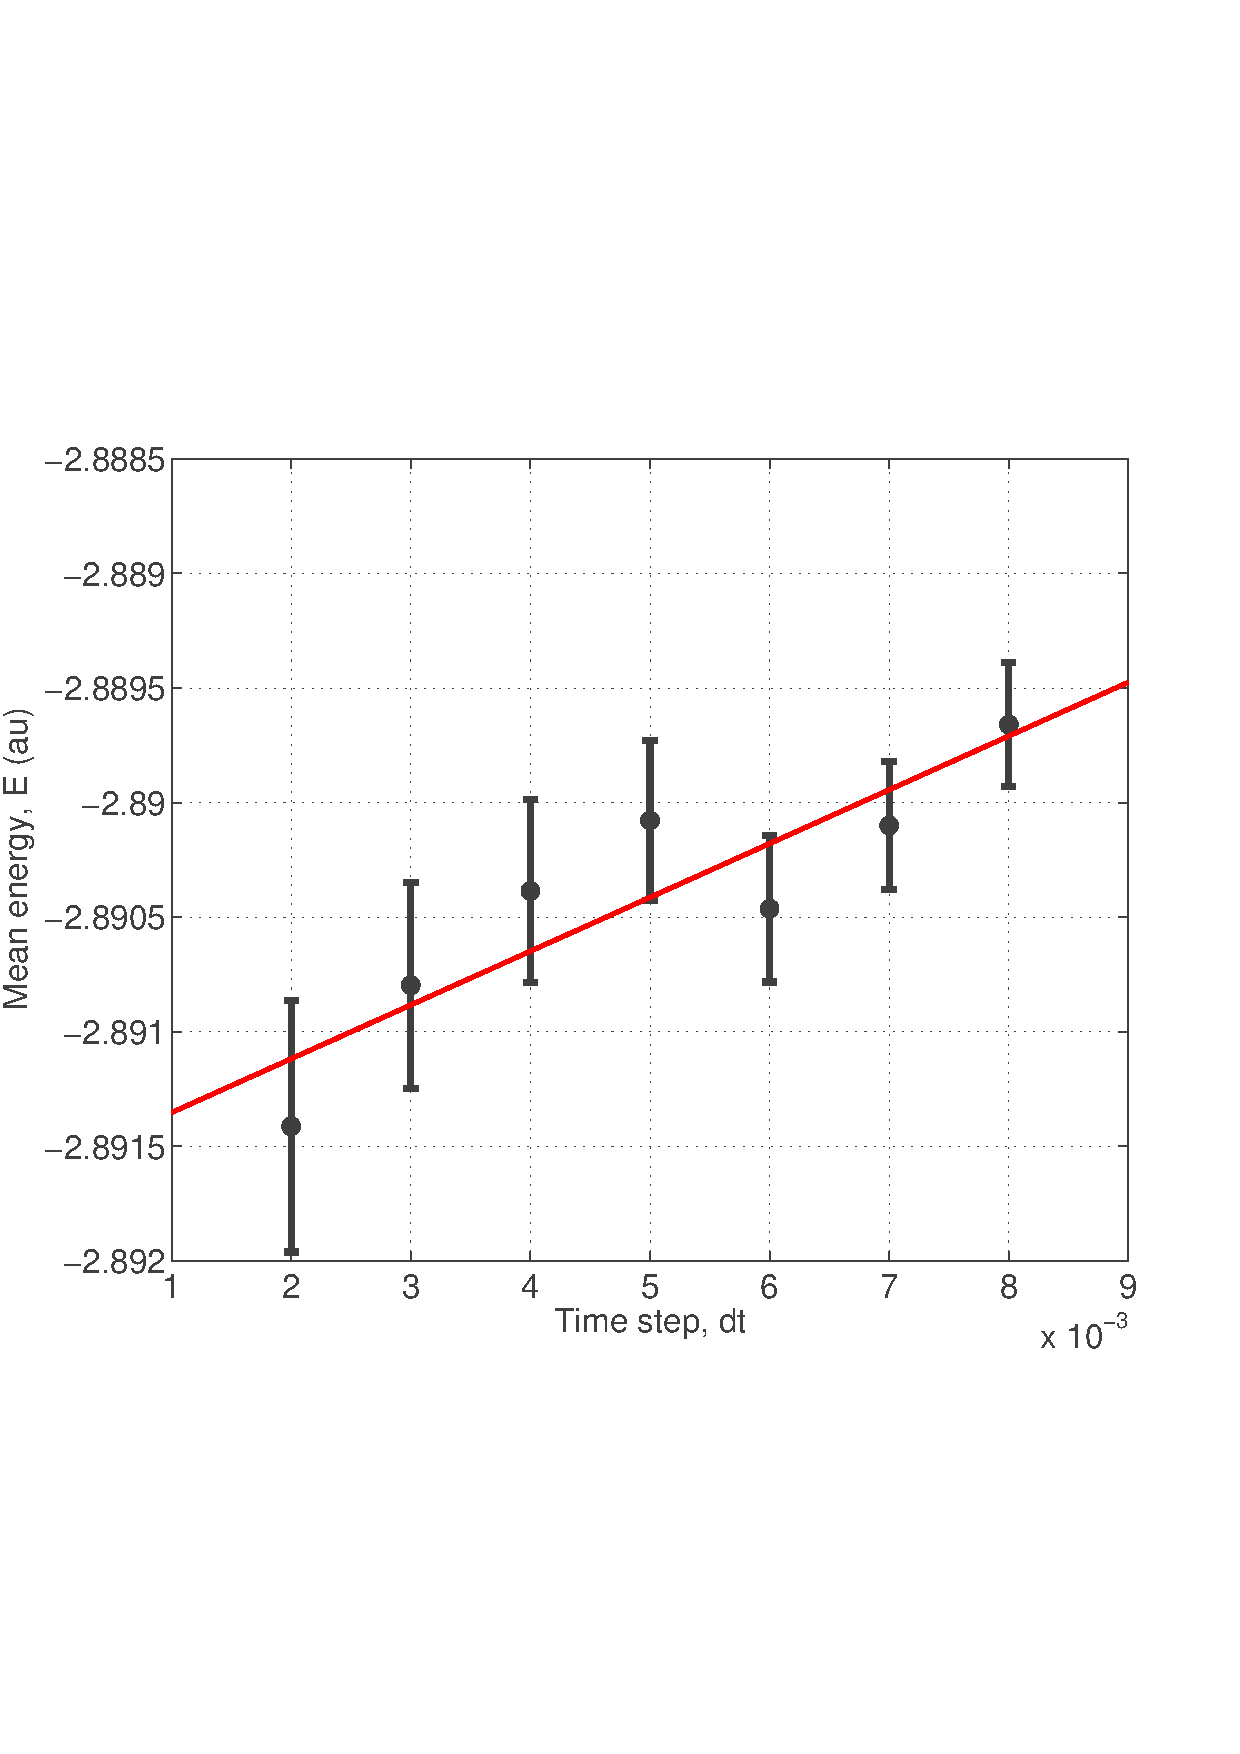
\includegraphics{experimentalData/blocking/He/blockingDtHe}} &
		 \resizebox{75mm}{!}{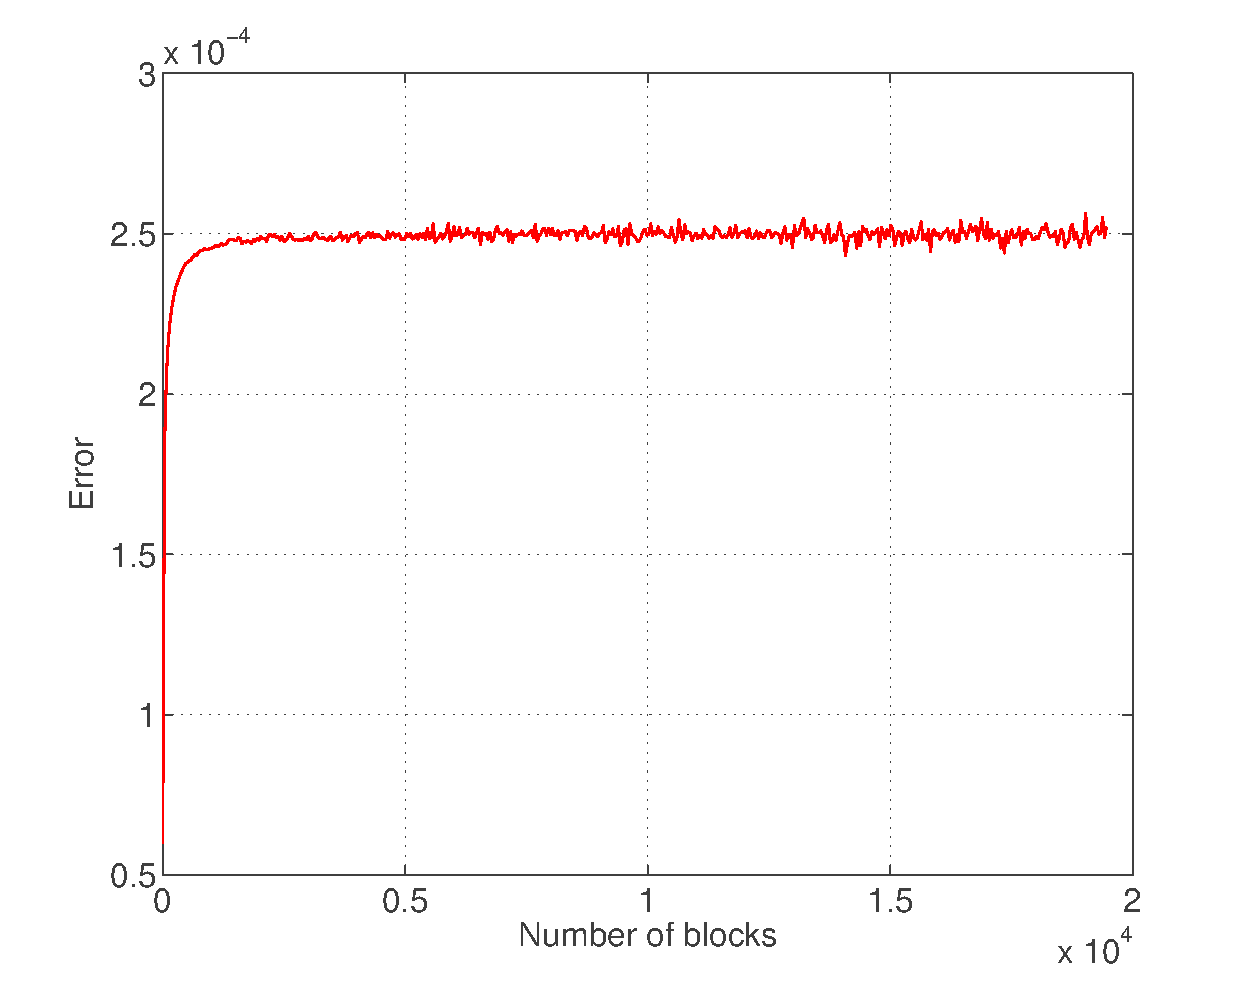
\includegraphics{experimentalData/blocking/blockingHe}} \\
		 \end{tabular}
		\caption{To the left we show the  extrapolation to $dt-$zero of the energy for a He atom. To the  right we display the details of the blocking analysis at $dt=0.01$ where the energy $-2.89039 \pm 2.5 \times 10^{-4}\, au$. Experimental setup: $10^7$ Monte Carlo cycles, $10 \%$ equilibration steps with four nodes, with $\alpha = 1.8379$, $\beta = 0.3704$.}
		\label{dtEnergyExtrapolationHe}
	\end{center}
\end{figure}

\begin{figure}[!hbt]
	\begin{center}
		\begin{tabular}{cc}
		\resizebox{75mm}{!}{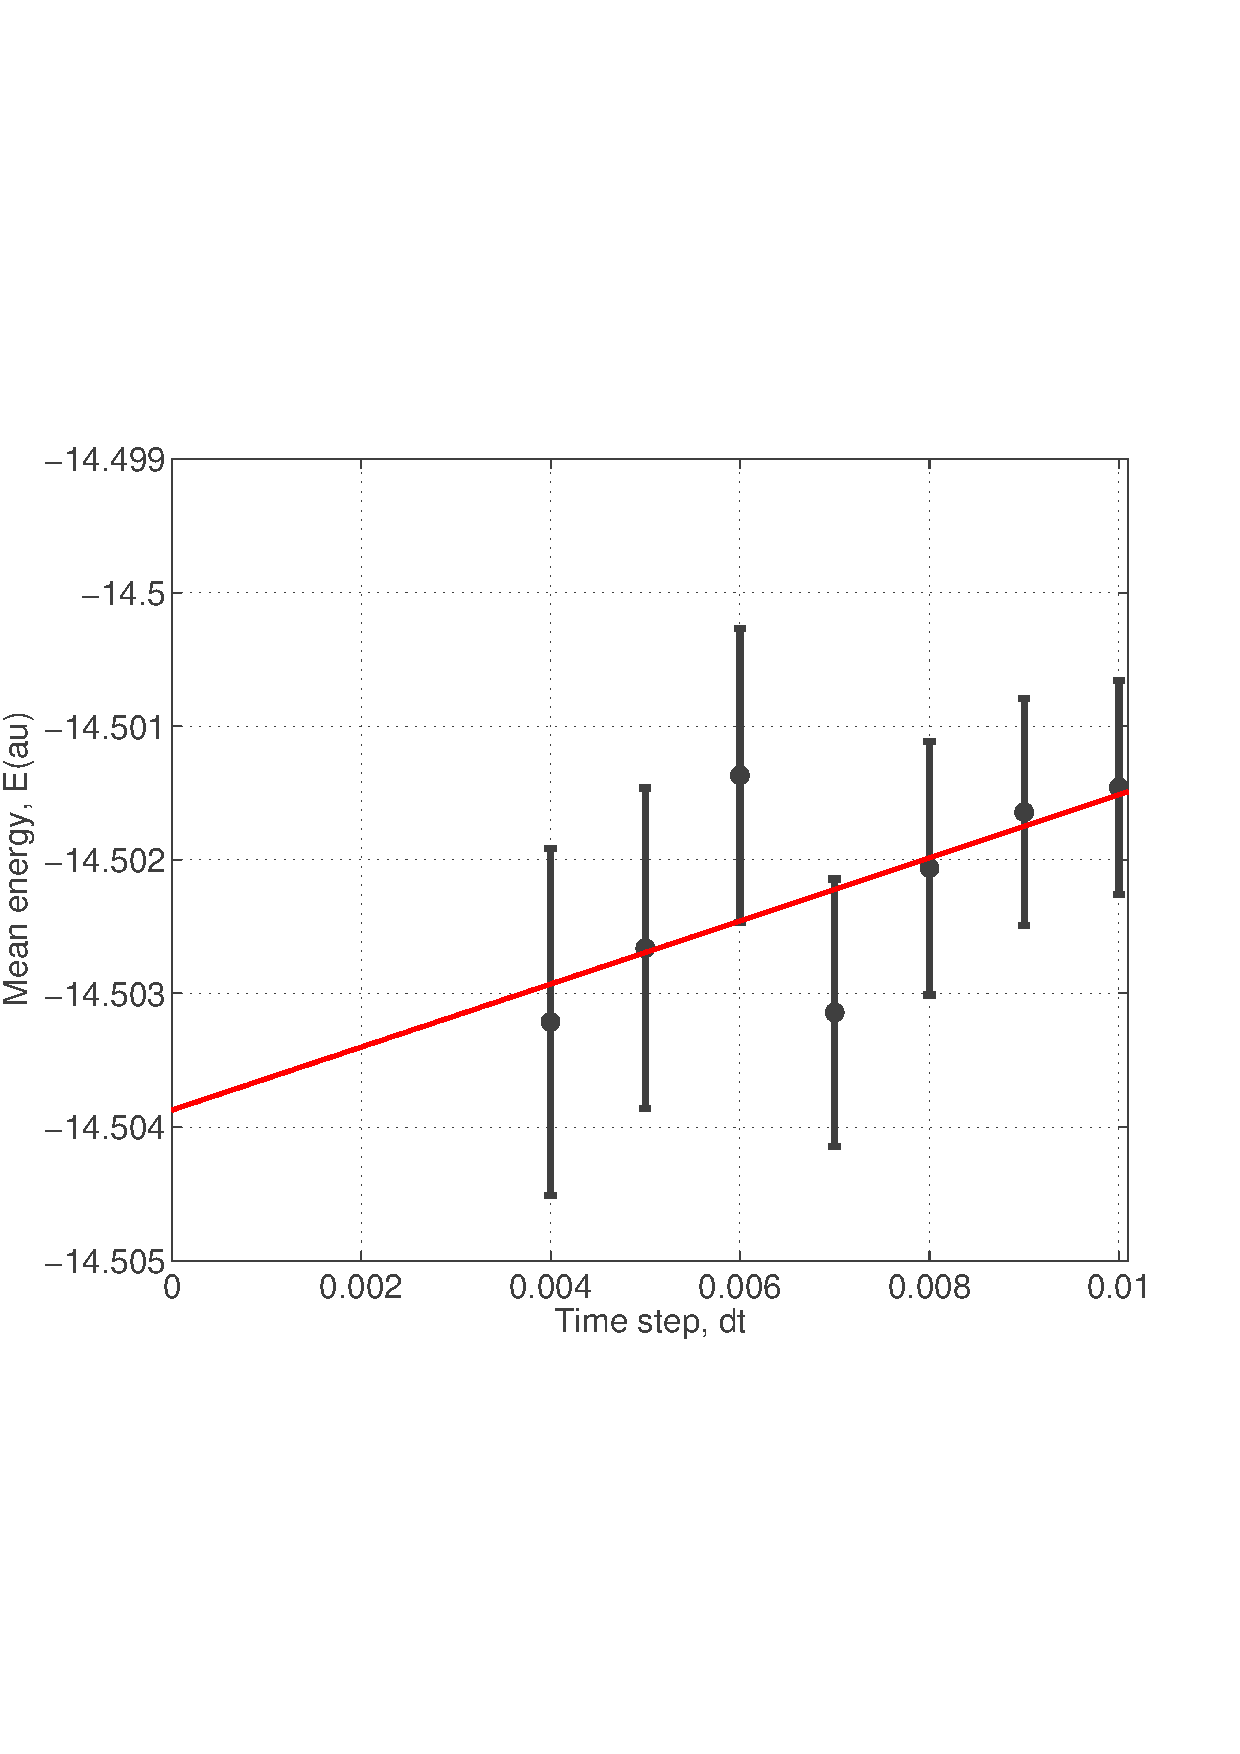
\includegraphics{experimentalData/blocking/Be/blockingDtBe}} &
		\resizebox{75mm}{!}{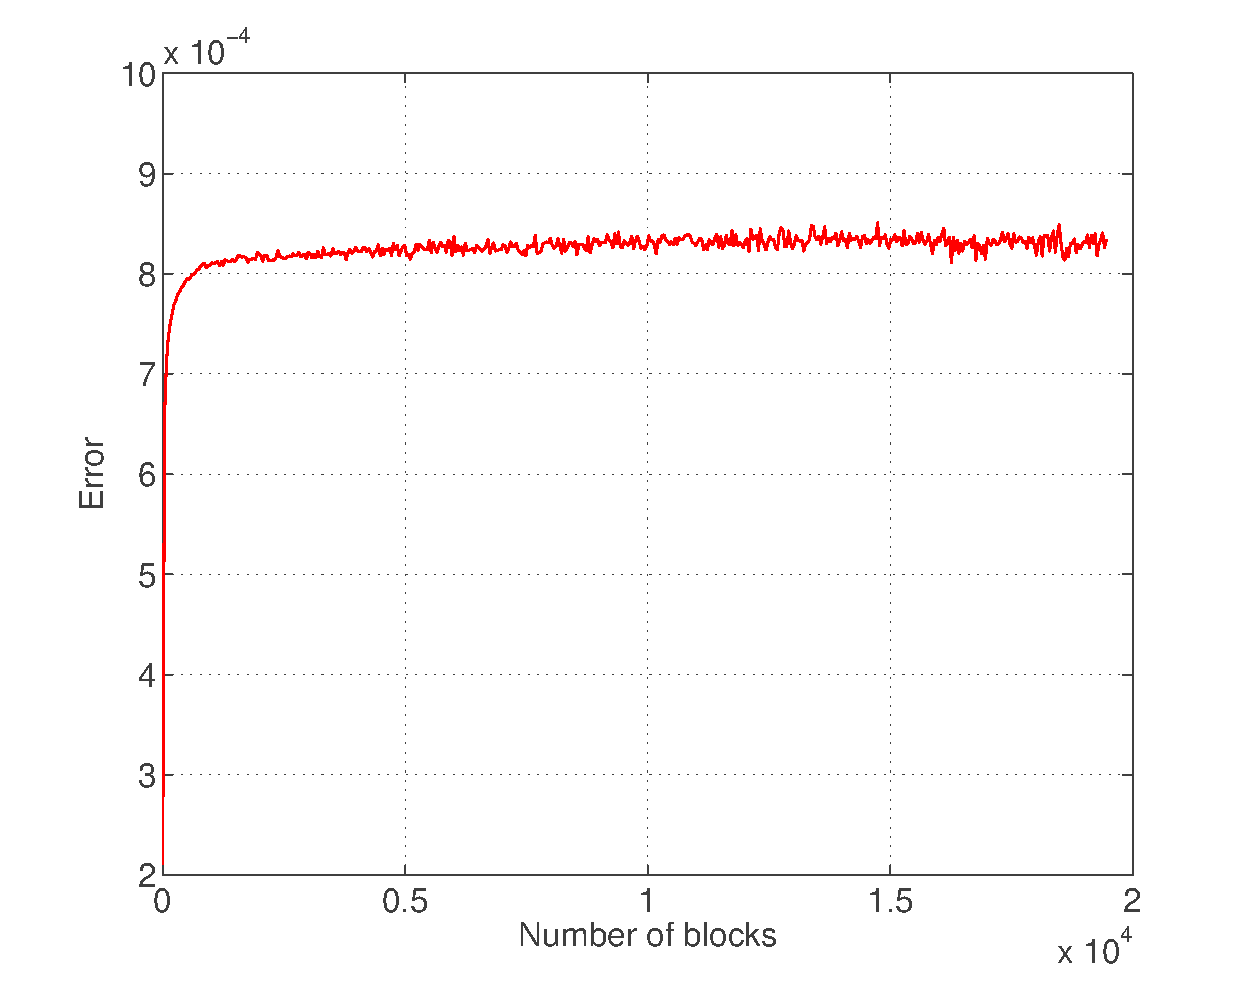
\includegraphics{experimentalData/blocking/plotBlockingBe}} \\
		\end{tabular}
		\caption{Extrapolation to $dt-$zero of the energy (left) and blocking analysis at $dt=0.01$ for the Be atom where the energy $E = -14.50146 \pm 8.5 \times 10^{-4} \, au$. Experimental setup: $10^7$ Monte Carlo cycles, $10 \%$ equilibration steps for four nodes, with $\alpha = 3.983$ and $\beta = 0.103$.}
		\label{dtEnergyExtrapolationBe}
	\end{center}
\end{figure}

\noindent
Allocating the region with quasi-linear $energy-dt$ dependence is computationally costly because of the number of evaluations (in parallel) required to explore the domain of $dt$. Fixing the seed in the random generator and reducing the number of Monte Carlo cycles is a straigforward way of allocating such a domain. This exploration could be done as a serial computation as well. It could be used later to produce results with a random seed and in parallel. \\
\\

\noindent
Tables \ref{blockingDtTableHe} to \ref{blockingDtTable2DQDot6e} present values of energies as a function of $dt$ as well as the percentage of accepted moves for the systems studied in this thesis. This percentage is inversly proportional with $dt$ in the region with a quasi-linear $energy-dt$ dependence. Moreover, it remains above 99 \%. In the same domain, the step sizes observed for quantum dots are longer than for atoms, indicating that systems with bigger length scales require longer jumps in $dt$ to cover a bigger configuration space during the sampling process. \\


\begin{figure}[!hbt]
	\begin{center}
		\begin{tabular}{cc}
		\resizebox{75mm}{!}{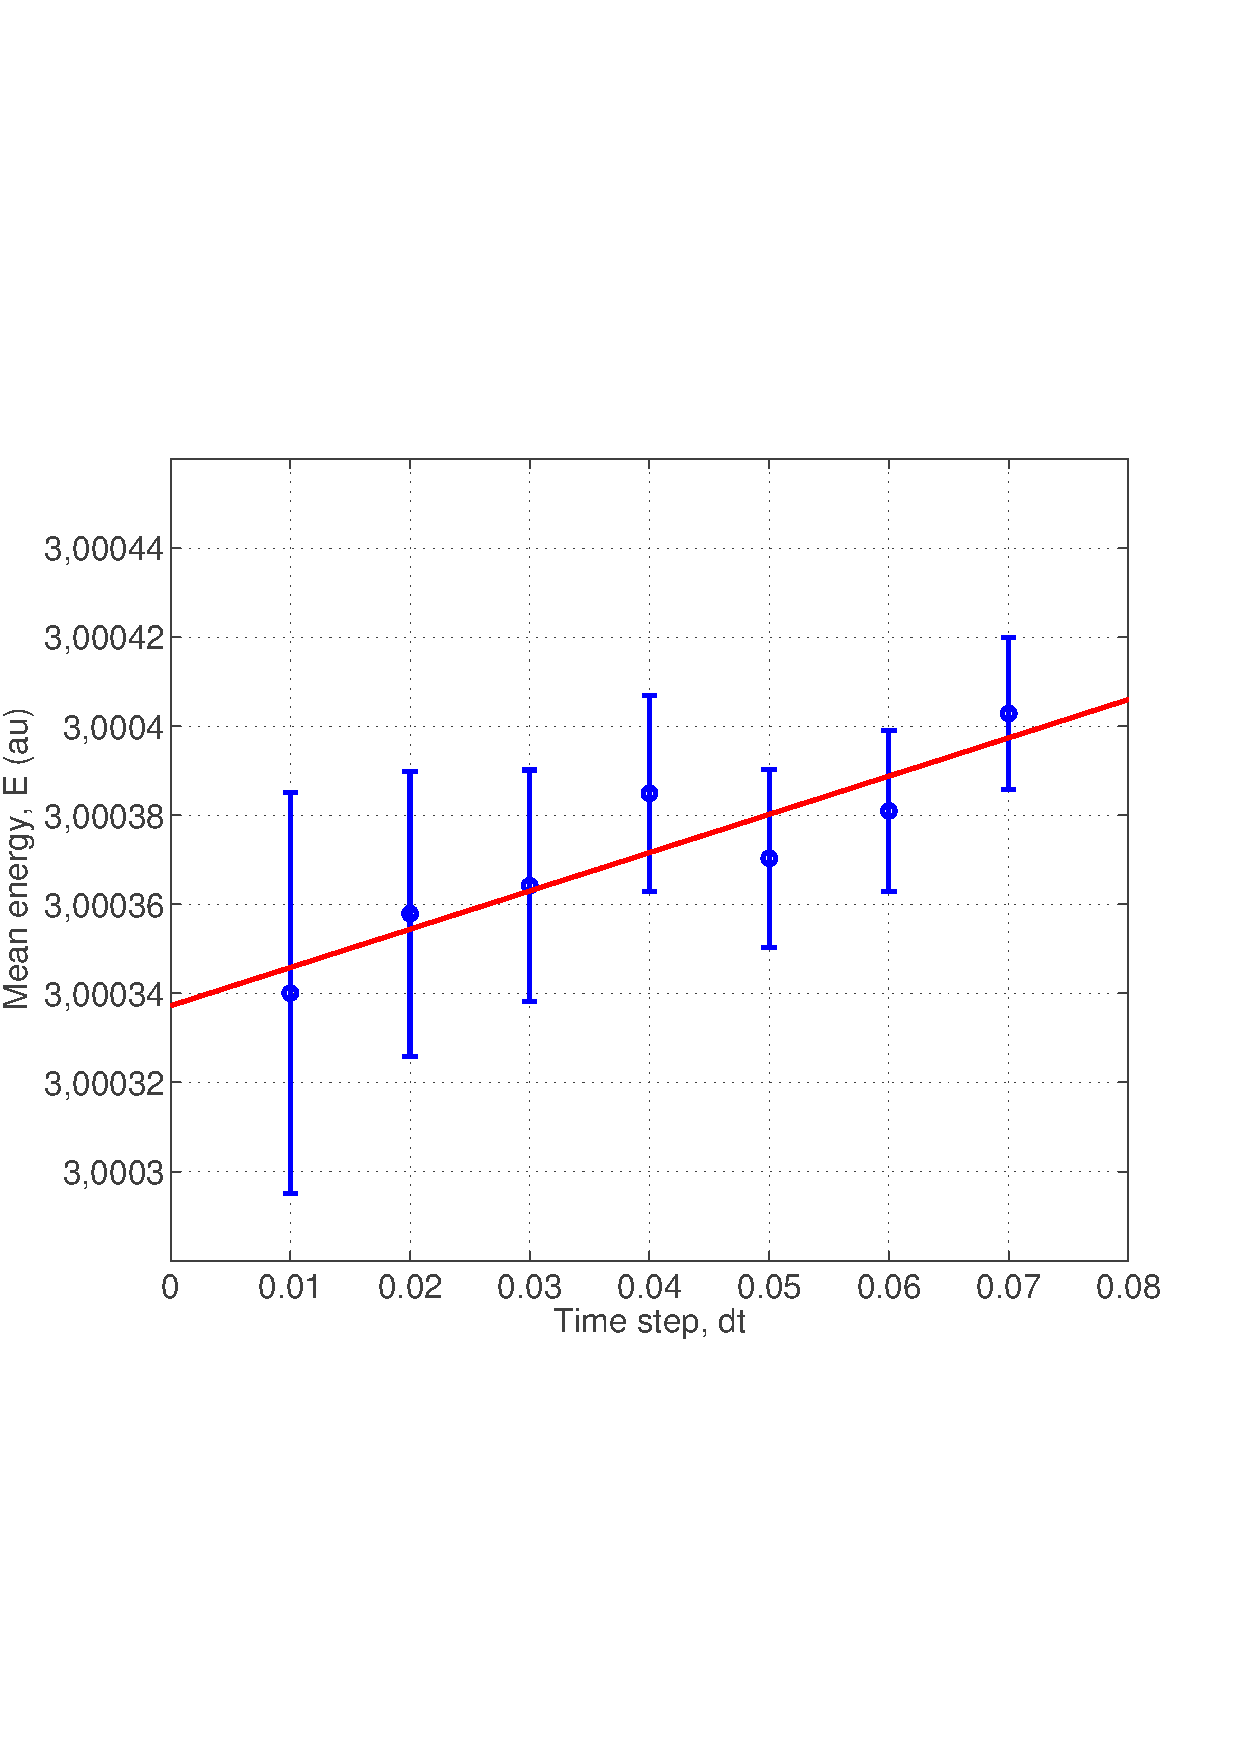
\includegraphics{experimentalData/secondPart/dtStudy2DQDot2e/dtPlot2DQDot2e}} &
		\resizebox{75mm}{!}{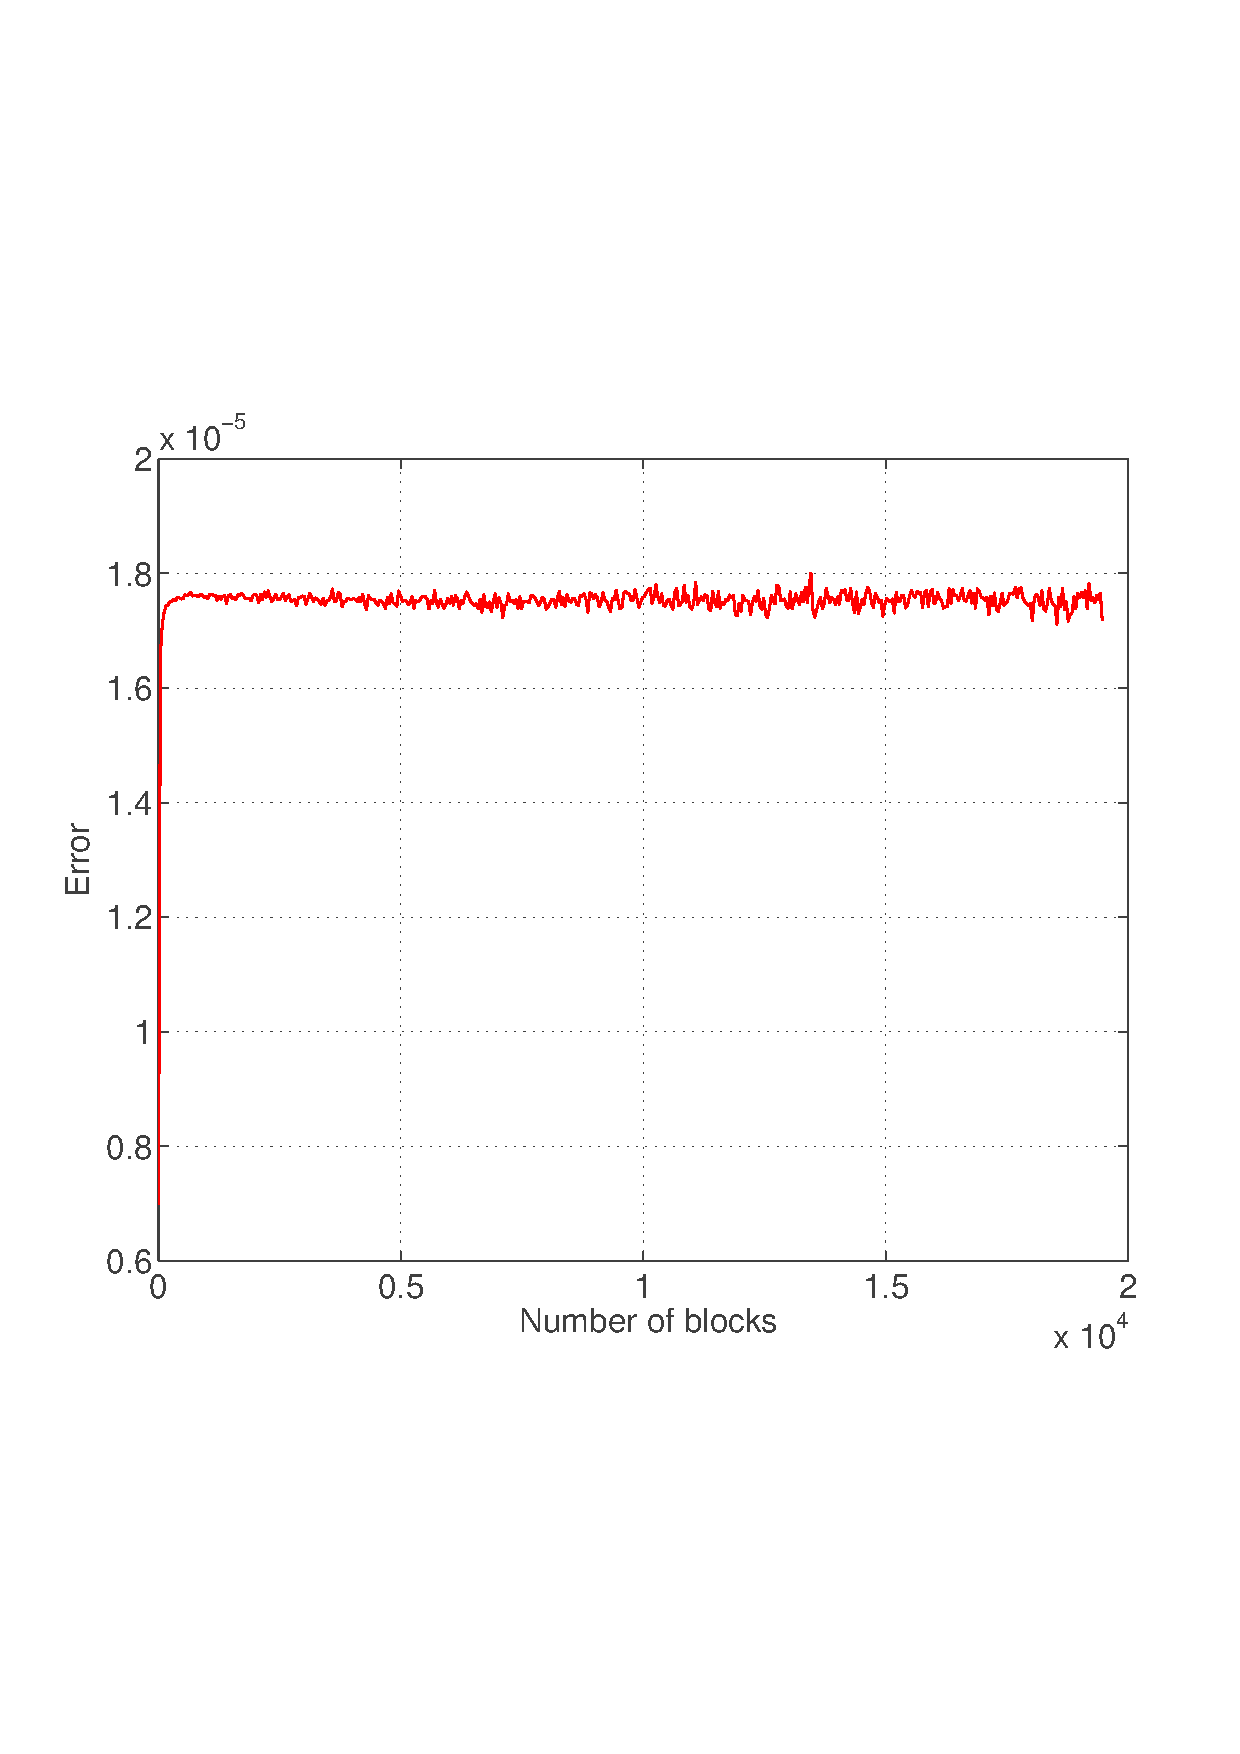
\includegraphics{experimentalData/blocking/2DQDot2e/block2DQDot2edt0p06}} \\
		\end{tabular}
		\caption{Extrapolation to $dt-$zero of the energy for a two-dimensional quantum dot with two electrons (left) and mean energy error ($E_{min} = 3.000381 \pm 1.8 \times 10^{-5} \, au$) at $dt=0.06$ as a function of the number of blocks for a 2DQDot2e (right). Parameters of simulation: $1 \times 10^7$ Monte Carlo steps with 10 \% equilibration steps, $\alpha = 0.99044$ and $\beta = 0.39994$. The error varies from $1.7 \times 10^{-5}$ at $dt = 0.07$ to $4.5\times 10^{-5}$ at $dt = 0.01$.}
		\label{dtEnergyExtrapolation2DQdot2e}
	\end{center}
\end{figure}



\begin{figure}[!hbt]
	\begin{center}
		\begin{tabular}{cc}
		\resizebox{75mm}{!}{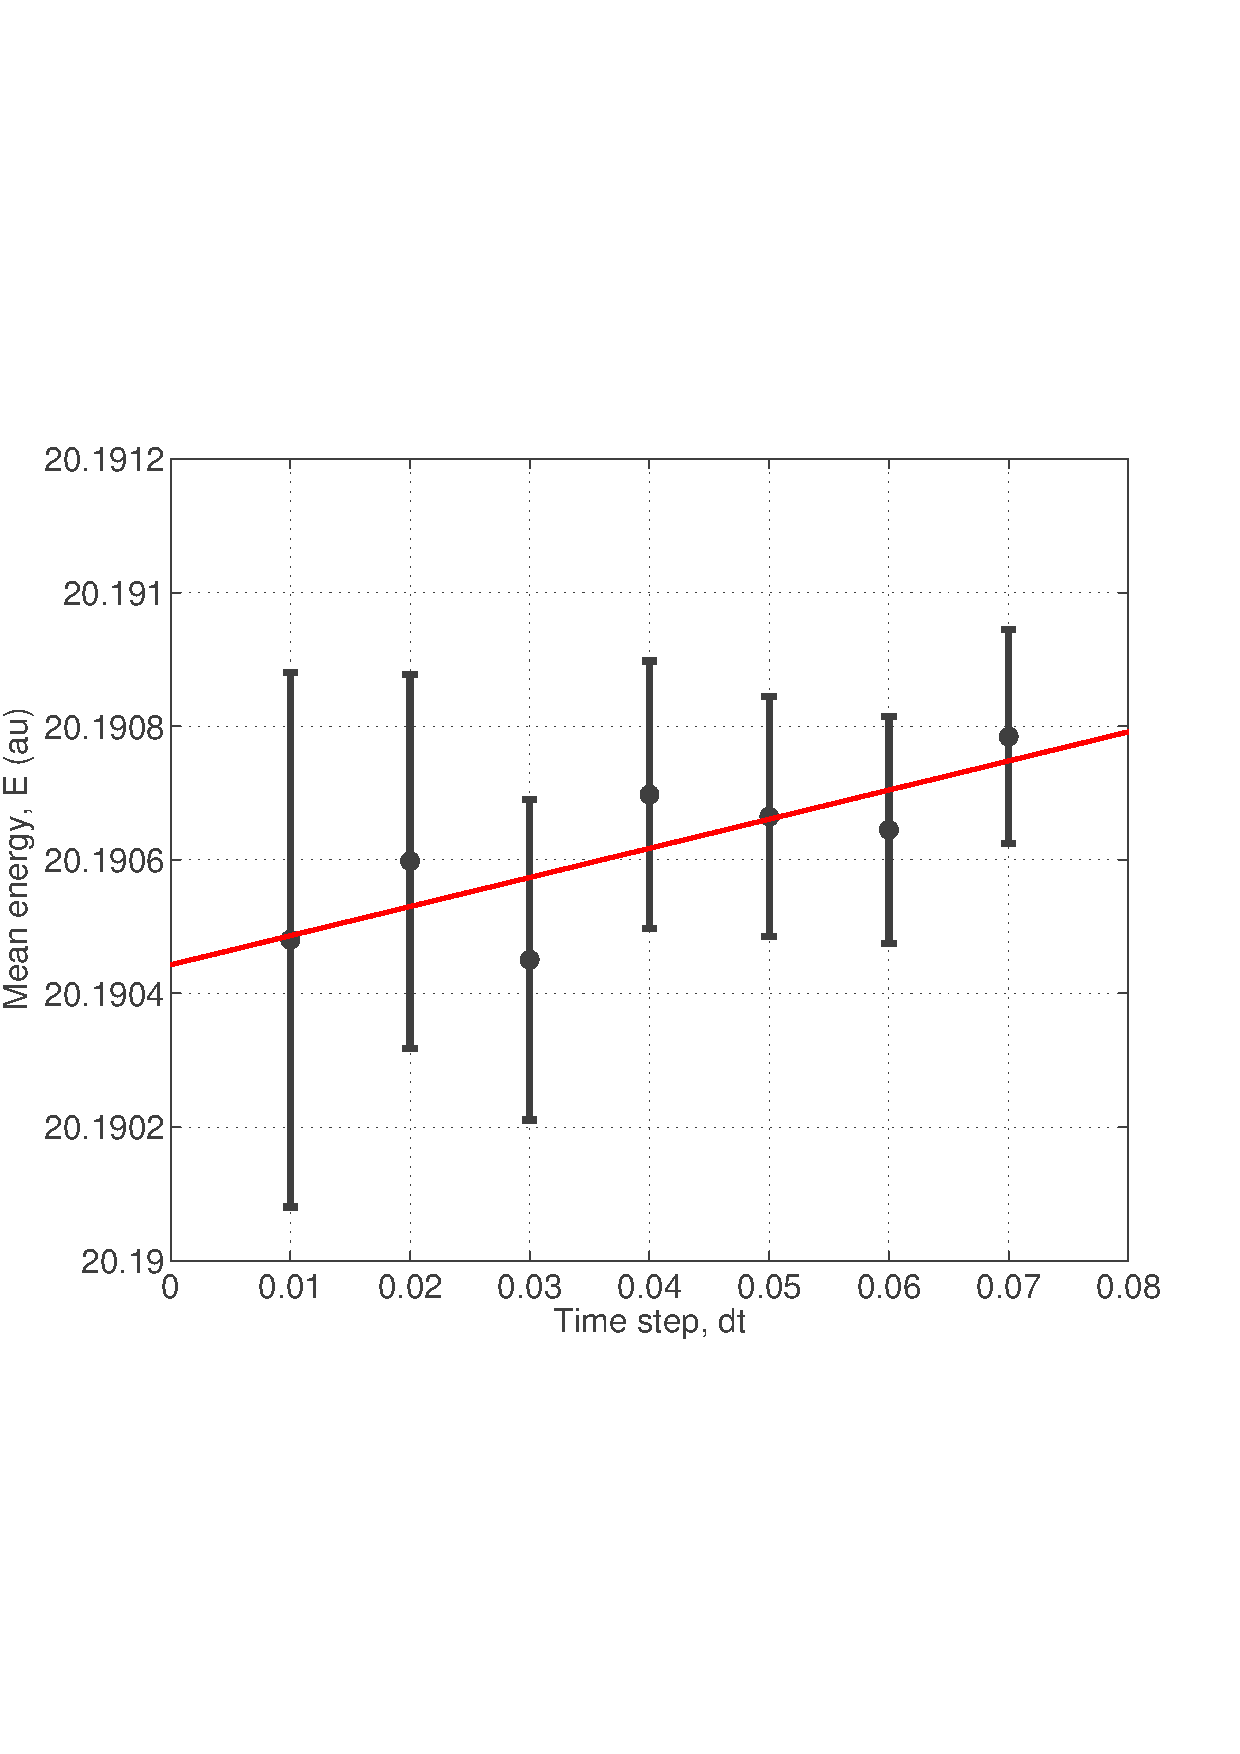
\includegraphics{experimentalData/blocking/plotDtStudy2DQDot6e}} &
		\resizebox{75mm}{!}{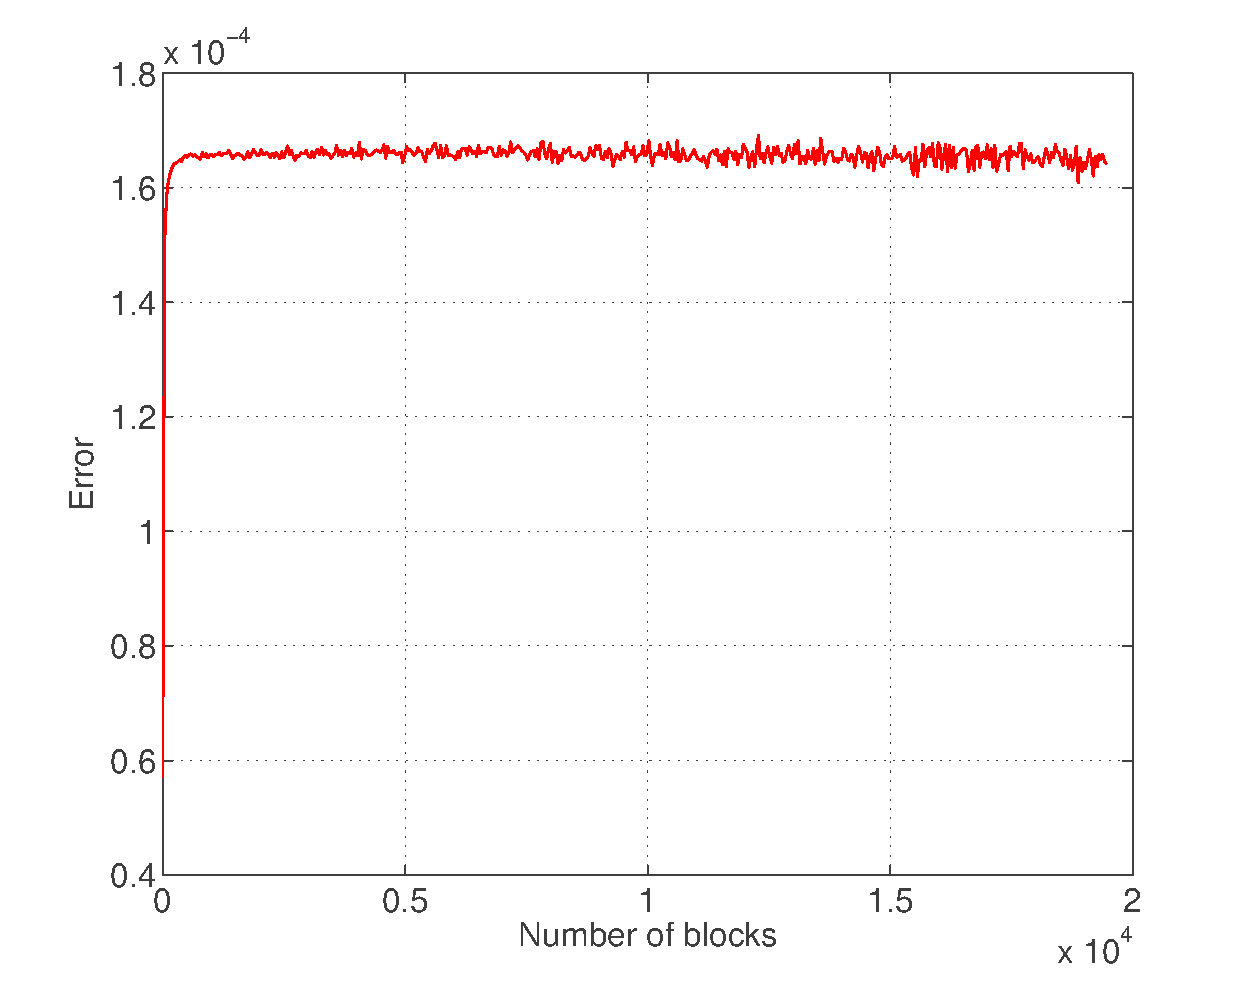
\includegraphics{experimentalData/blocking/2DQDot6e/blockAnalyse2DQDot6e}}\\
		\end{tabular}
		\caption{Extrapolation to $dt-$zero of the energy for a two-dimensional quantum dot with six electrons (left) and mean energy error ($E_{min} = 20.190645 \pm 1.7 \times 10^{-4} \, au$) at $dt=0.06$ as a function of the number of blocks for a 2DQDot6e (right). Parameters of simulation: $10^7$ Monte Carlo steps with 10 \% equilibration steps, $\alpha = 0.926273$ and $\beta = 0.561221$ running with four nodes.}
		\label{dtEnergyExtrapolation2DQdot6e}
	\end{center}
	
	
\end{figure}


\begin{table}[!hbt]
\centering
\begin{tabular}{cccc}
\toprule[1pt]
\textbf{Time step} & \textbf{Energy}, (au) 	& \textbf{Error} & \textbf{Accepted moves}, (\%) \\
\midrule[1pt]
0.002  & -2.891412637854  &  5.5e-4   &  99.97\\
0.003  & -2.890797649433  &  4.5e-4   &  99.94\\
0.004  & -2.890386198895  &  4.0e-4   &  99.91\\
0.005  & -2.890078440930  &  3.5e-4   &  99.88\\
0.006  & -2.890463490951  &  3.2e-4   &  99.84\\
0.007  & -2.890100432462  &  2.8e-4   &  99.81\\
0.008  & -2.889659923905  &  2.7e-4   &  99.77\\
\bottomrule[1pt]
\end{tabular}\caption{Energy computed for the He atom and the error associated as a function of the time step. Parameters: $10^7$ Monte Carlo cycles with 10 \% equilibration steps, $\alpha =  1.8379$ and $\beta = 0.3704$.}\label{blockingDtTableHe}
\end{table}




\begin{table}[!hbt]
\centering
\begin{tabular}{cccc}
\toprule[1pt]
\textbf{Time step} & \textbf{Energy}, (au) 	& \textbf{Error} & \textbf{Accepted moves}, (\%) \\
\midrule[1pt]
0.004  & 	-14.50321303316  &  1.3e-3  &   99.61\\
0.005  & 	-14.50266236227  &  1.2e-3  &   99.47\\
0.006  & 	-14.50136820967  &  1.1e-3  &   99.32\\
0.007  & 	-14.50314292468  &  1.0e-3  &   99.17\\
0.008  & 	-14.50206184582  &  9.5e-4  &   99.01\\
0.009  & 	-14.50164368104  &  8.5e-4  &   98.85\\
0.01   & 	-14.50145748870  &  8.0e-4  &   98.68\\
\bottomrule[1pt]
\end{tabular}\caption{Energy computed for the Be atom and the error associated as a function of the time step. Parameters: $10^7$ Monte Carlo cycles with 10 \% equilibration steps, $\alpha = 3.983$ and $\beta = 0.103$.}\label{blockingDtTableBe}
\end{table}


	
\begin{table}
\centering
\begin{tabular}{cccc}
\toprule[1pt]
\textbf{Time step} & \textbf{Energy}, (au) 	& \textbf{Error} & \textbf{Accepted moves}, (\%) \\
\midrule[1pt]
0.01 & 3.000340072477 & 4.5e-5 & 99.95\\
0.02 & 3.000357900850 & 3.2e-5 & 99.87\\
0.03 & 3.000364180564 & 2.6e-5 & 99.77\\
0.04 & 3.000384908560 & 2.2e-5 & 99.65\\
0.05 & 3.000370330692 & 2.0e-5 & 99.52\\
0.06 & 3.000380980039 & 1.8e-5 & 99.37\\
0.07 & 3.000402836533 & 1.7e-5 & 99.21\\
\bottomrule[1pt]
\end{tabular}\caption{Results of a blocking analysis for several time steps. The system was a two-dimensional quantum dot with two electrons and $\omega=1.0$. The rest of the parameters were: $10^7$ Monte Carlo cycles with 10 \% equilibration steps, and $\alpha = 0.99044$ and $\beta = 0.39994$ taken from reference\cite{Albrigtsen}.}\label{blockingDtTable2DQDot2e}
\end{table}





\begin{table}
\centering
\begin{tabular}{cccc}
\toprule[1pt]
\textbf{Time step} & \textbf{Energy}, (au) 	& \textbf{Error} & \textbf{Accepted moves}, (\%) \\
\midrule[1pt]
0.01 & 20.19048030567 & 4.0e-4 & 99.90\\
0.02 & 20.19059799459 & 2.8e-4 & 99.75\\
0.03 & 20.19045049792 & 2.4e-4 & 99.55\\
0.04 & 20.19069748408 & 2.0e-4 & 99.34\\
0.05 & 20.19066469178 & 1.8e-4 & 99.10\\
0.06 & 20.19064491561 & 1.7e-4 & 98.85\\
0.07 & 20.19078449010 & 1.6e-4 & 98.58\\
\bottomrule[1pt]
\end{tabular}\caption{Results of a blocking analysis for several time steps. The system was a two-dimensional quantum dot with six electrons and $\omega=1.0$. The rest of the parameters were: $10^7$ Monte Carlo cycles with 10 \% equilibration steps, and $\alpha = 0.926273$ and $\beta = 0.561221$ taken from reference\cite{Albrigtsen}.}\label{blockingDtTable2DQDot6e}
\end{table}

\noindent
The results for the  energy of atoms and 2DQDot2e using extrapolation to zero $dt$ shown in table \ref{energyCuts} are in correspondence with values listed in the scientific literature, see for example Refs.~\cite{alexander1997, taut1994}. In general, the difference between the lowest and highest energies were small. Doing an extrapolation to zero can be expensive in terms of the computational time involved in doing blocking for each $dt$, and is practical for big systems. One should evaluate the gain of getting some decimals digits in energy against the computational cost required by the computation. \\
\\

\begin{table}
\centering
\begin{tabular}{lr}
\toprule[1pt]
\textbf{System} & \textbf{Energy}, (au)\\
\midrule[1pt]
He &  -2.8913\\
Be &  -14.5039\\
2DQDot2e & 3.0003\\
2DQDot6e & 20.1904\\
\bottomrule[1pt]
\end{tabular}\caption{Energies estimated using zero-dt extrapolation in figures  \ref{blockingDtTableHe} to \ref{blockingDtTable2DQDot6e}. $\omega~=~1.0$ for quantum dots.}\label{energyCuts}
\end{table}

\noindent 
In relation with the figures \ref{dtEnergyExtrapolationHe} to \ref{dtEnergyExtrapolation2DQdot6e}(right), in all the cases the amplitude of the oscillations in the error increases with the number of blocks, reflecting the fact that the greater the number of blocks is, the greater the sequential correlation in the set of correlated energy data becomes, because of the reduction of the distance between the $i^{th}-$entry in each block. \\
\\
\noindent
Later, the blocking analysis shows also that the greater the system, the greater the error in energy is for equal number of Monte Carlo cycles and spatial dimensions, simply due to the fact that the number of degrees of freedom and the role of correlations increase with the size of the system. \\
\\
\noindent
The effect of the interelectronic correlaton will, however, have less impact in higher dimensions. At lower dimensions the particles have less degrees of freedom to avoid each other, but make it more difficult for more than two particles to get close to each other.


\section{Error as a function of the number of Monte Carlo cycles in Be atom}

In this experiment we were interested in finding the behaviour of the error as a function of the number of Monte Carlo cycles. The runs were executed with a Be atom with fixed seed (in the random number generator). Figures \ref{errorVsMcBe} (right and left) show the error decaying exponentially after which it stabilizes, indicating that no much gain in the reduction of the error in reached by increasing the number of Monte Carlo cycles (and computational cost).

\begin{figure}[!hbt]
    \begin{center}
			 \begin{tabular}{cc}
			\resizebox{75mm}{!}{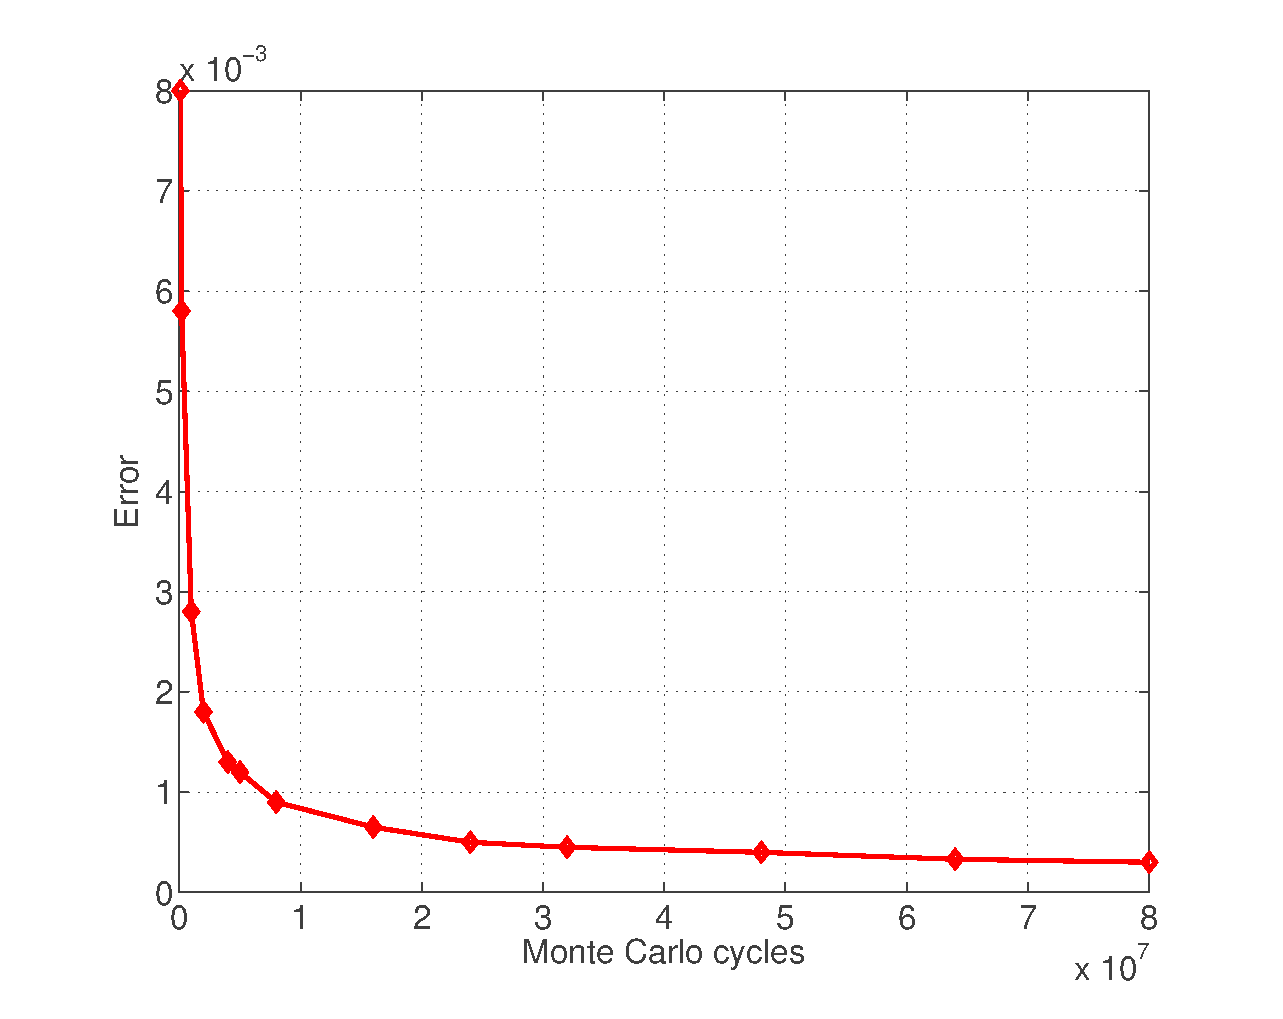
\includegraphics{experimentalData/secondPart/errorVsMCBe/errorVsMonteCarloBe}}
			\resizebox{75mm}{!}{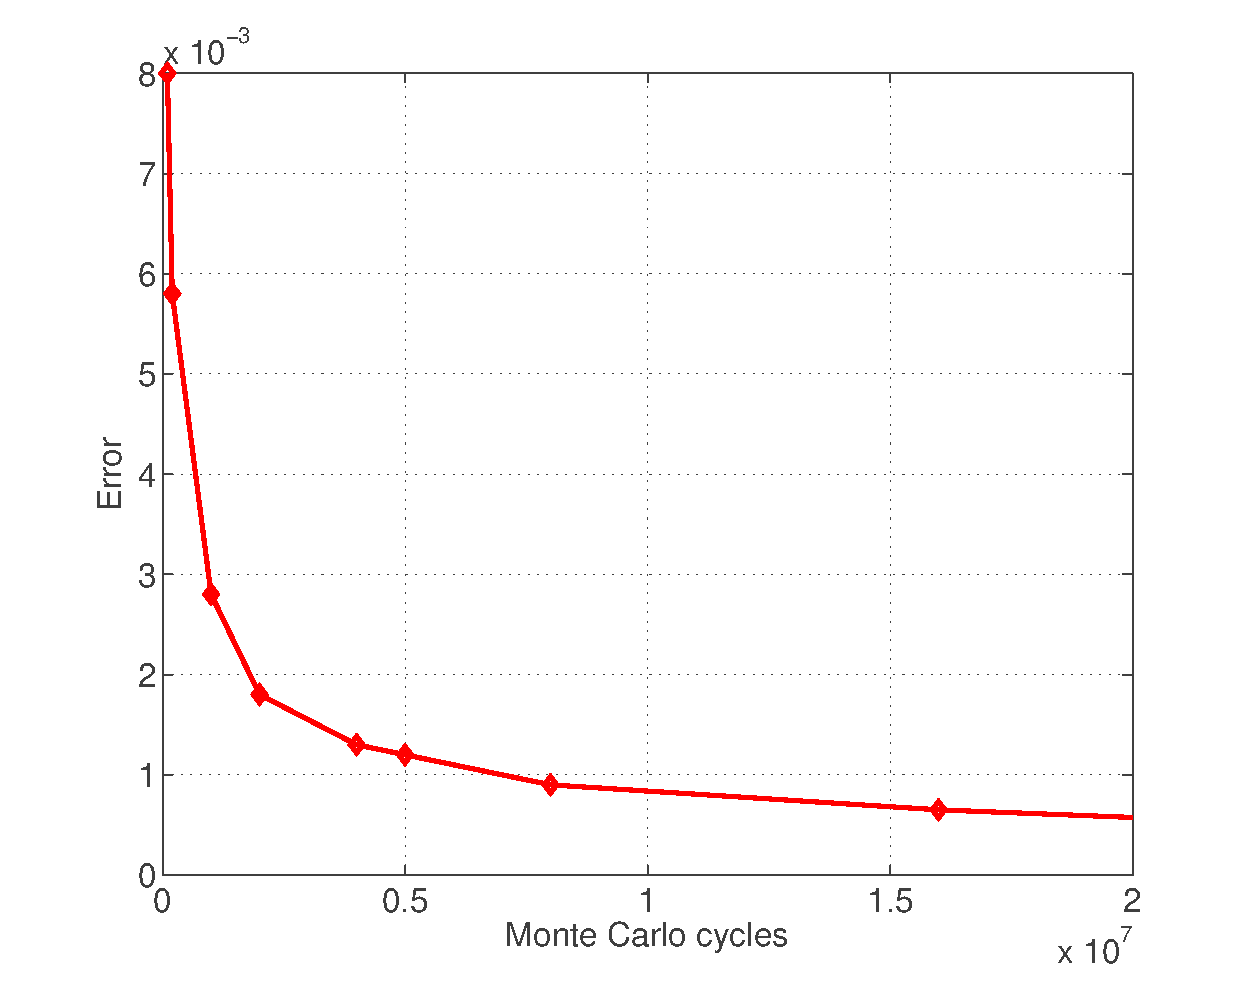
\includegraphics{experimentalData/secondPart/errorVsMCBe/errorVsMonteCarloBeZoom}}\\
			 \end{tabular}
      \caption{Error in the energy (left) and zoom(right) obtained by blocking for a Be atom as a function of the number of Monte Carlo cycles. The set up for the experiment was: $dt = 0.01$, $\alpha = 3.981$, $\beta = 0.09271$ and 10 \% equilibration steps by run.}
      \label{errorVsMcBe}
    \end{center}
  \end{figure}


% \section{Dependence of the optimum variational parameters alpha on the oscillator frequency}

% % % % % % EN LA DESCRIPCION DEL PROBLEMA: Esta son matrices cuadradas de tamanno $N^2$. Para una particula tendremos 1x1, para 2x2=4 pero para 4x4=16. 
% % % % % % \section{Influence of the percent of thermalization steps in the convergence of the vmc method to the ground state energy and optimization}
% % % % % % 
% % % % % % Mirar si esto refleja que el methodo de quasi Newton es altamente sensible al noise, supuestamente reducido introduciendo thermalization. Es decir que uno esperaria que incrementando la termalizacion la convergencia de los parameteros dadno la minima energfia mejore.
% % % % % % 
% \section{Importance of the percentage of thermalizations on the reduction of the error}
% \section{Benchmarks: analysis of speed of different parts of the code}
% % % % % -analizar la posibilidad de incluuir multinivel.


\clearemptydoublepage
